% Searching and retrieving along-track altimetry: the aicesat design, from the data up.
% Build (in docs/):  xelatex -interaction=nonstopmode -halt-on-error functional-design.tex
%                    bibtex functional-design
%                    xelatex -interaction=nonstopmode -halt-on-error functional-design.tex   (twice more)
% Needs xelatex with the system fonts Palatino and Menlo (TeX Live 2026 basic + fontspec is enough).
\documentclass[10pt,a4paper]{article}

\usepackage[a4paper,textwidth=112mm,marginparwidth=46mm,marginparsep=7mm,left=22mm,top=24mm,bottom=28mm,
            footskip=12mm]{geometry}
\usepackage{fontspec}
\setmainfont{Palatino}
\linespread{1.06}
\setmonofont{Menlo}[Scale=0.82]
\usepackage{microtype}
\usepackage{amsmath,amssymb}
\usepackage{booktabs,array}
\usepackage{xcolor}
\usepackage{tikz}
\usetikzlibrary{positioning,arrows.meta,fit,calc,shapes.geometric,backgrounds,decorations.pathreplacing,matrix}
\usepackage{caption}
\usepackage{listings}
\usepackage{fancyvrb}
\usepackage{ragged2e}
\usepackage{parskip}
\setlength{\emergencystretch}{1.5em}
\usepackage[numbers,sort&compress]{natbib}
\usepackage{url}
\usepackage[hidelinks]{hyperref}

% ---- colours: one ink, one soft grey, one panel, one accent, one for the remote side ---------------------------
\definecolor{ink}{HTML}{2B2B2B}
\definecolor{soft}{HTML}{6B7A8D}
\definecolor{panel}{HTML}{F1F4F8}
\definecolor{idxblue}{HTML}{2F6FED}
\definecolor{nasared}{HTML}{C0504D}

\captionsetup{font=small,labelfont=bf,justification=RaggedRight,singlelinecheck=false,skip=6pt}
\setlength{\itemsep}{1pt}
\setlength{\marginparpush}{6pt}
\setcounter{topnumber}{3}\setcounter{totalnumber}{4}
\renewcommand{\topfraction}{0.9}\renewcommand{\textfraction}{0.05}\renewcommand{\floatpagefraction}{0.6}

% ---- margin notes --------------------------------------------------------------------------------------------
\newcounter{sidenote}
\newcommand{\side}[1]{\stepcounter{sidenote}\textsuperscript{\thesidenote}%
  \marginpar{\RaggedRight\footnotesize\textsuperscript{\thesidenote}\,#1}}
\newcommand{\mnote}[1]{\marginpar{\RaggedRight\footnotesize #1}}
\newcommand{\todaynote}{\textit{what exists today.}}
\newcommand{\landed}[1]{\mnote{\todaynote\ #1}}

% ---- code ----------------------------------------------------------------------------------------------------
\newcommand{\code}[1]{\texttt{#1}}
\lstdefinestyle{py}{language=Python,basicstyle=\ttfamily\footnotesize,keywordstyle=\bfseries,
  commentstyle=\color{soft}\itshape,stringstyle=\color{ink},columns=fullflexible,keepspaces=true,
  showstringspaces=false,breaklines=true,frame=none,xleftmargin=0pt,aboveskip=4pt,belowskip=4pt,
  morekeywords={frozen,slots,dataclass}}
\lstset{style=py}
\fvset{fontsize=\footnotesize,baselinestretch=1.0}

% ---- figure grammar (one definition, every figure) -----------------------------------------------------------
\tikzset{
  val/.style   = {rectangle, draw=ink, fill=white, line width=0.6pt, inner sep=4pt, align=center, font=\footnotesize},
  pure/.style  = {rectangle, rounded corners=4pt, draw=ink, fill=white, line width=0.6pt, inner sep=5pt,
                  align=center, font=\footnotesize},
  eff/.style   = {rectangle, rounded corners=4pt, draw=ink, dashed, fill=panel, line width=0.6pt, inner sep=5pt,
                  align=center, font=\footnotesize},
  store/.style = {cylinder, shape border rotate=90, aspect=0.22, draw=ink, fill=panel, line width=0.6pt,
                  inner sep=3pt, align=center, font=\footnotesize},
  remote/.style= {cylinder, shape border rotate=90, aspect=0.22, draw=nasared, fill=nasared!6, line width=0.6pt,
                  inner sep=3pt, align=center, font=\footnotesize, text=nasared!80!black},
  proc/.style  = {rectangle, draw=soft, dashed, line width=0.5pt, inner sep=7pt, rounded corners=2pt},
  lane/.style  = {rectangle, fill=panel, draw=none},
  flow/.style  = {-{Stealth[length=2mm]}, line width=0.6pt, draw=ink},
  flowsoft/.style = {-{Stealth[length=2mm]}, line width=0.5pt, draw=soft},
  lbl/.style   = {font=\scriptsize, text=soft, align=center, inner sep=1pt},
  lblw/.style  = {font=\scriptsize, text=soft, align=center, inner sep=1pt, fill=white},
  note/.style  = {font=\scriptsize\itshape, text=soft, align=left},
  hdr/.style   = {font=\scriptsize\bfseries, text=ink, anchor=west},
  acc/.style   = {draw=idxblue, text=idxblue!85!black},
}
% a hexagon path: centre x, centre y, circumradius, rotation (plain numbers in the picture's units)
\newcommand{\hexp}[4]{%
  ({#1+#3*cos(#4)},{#2+#3*sin(#4)})
  \foreach \kk in {1,...,5} {-- ({#1+#3*cos(#4+60*\kk)},{#2+#3*sin(#4+60*\kk)})} -- cycle
}
% a full-width figure body: overflows into the margin column on purpose
\newcommand{\wide}[1]{\noindent\makebox[\textwidth][l]{#1}}
% requirement tags (Chapter 6) and the grid / track strokes used by the data and grid figures
\newcommand{\req}[1]{\textbf{R#1}}
\tikzset{
  grid/.style  = {draw=soft!60, line width=0.4pt},
  track/.style = {draw=idxblue, line width=0.9pt},
  foot/.style  = {fill=idxblue!55, draw=none},
  box/.style   = {draw=nasared, line width=0.7pt},
}

\title{\textbf{Searching and retrieving along-track altimetry}\\[4pt]
  \large a sub-granule index on a discrete global grid, and the engines that build and use it\\[2pt]
  \normalsize the aicesat design, from the data up}
\author{Kevin W. Beam}
\date{2026-10-18}

\begin{document}
\maketitle
\vspace{-2em}

\begin{abstract}
\noindent
We describe the characteristics of along-track, non-gridded altimetry data that make it difficult to search and
retrieve: data from ICESat's GLAS, Operation IceBridge's ATM, ICESat-2's ATLAS, GEDI, and a ground traverse, as
they are archived in the Earthdata cloud. Using a canonical set of searches and retrievals based on geospatial area,
temporal specification, and filtering and aggregating constraints, we show where granule-level search fails on such
data and derive, from first principles, what an efficient system must record. We build a system that transforms
granules and their metadata into an \emph{index into the raw data}. Taking into account the logical and physical
organisation of the files, we show how a discrete global grid system turns that index into a table that answers
spatial searches exactly and cheaply, and whose rows are request specifications: the byte ranges that hold the
matching points, retrievable from the granule files directly. We then describe the request engine that executes
those specifications and builds a local data lake from which analysis and visualisation proceed, and the framework
that lets each collection be a value plugged into one shared pipeline. Every number is a measurement on the deployed
instance; the margin records, chapter by chapter, which parts exist today.
\end{abstract}

\vspace{0.5em}

\section*{How to read this document}

The report proceeds in eight parts and is meant to be read in order. Part~I characterises the data: what an
along-track product is, how the archive packages it into granules, and how the bytes lie inside a granule.
Part~II states the problem: the queries the system is asked, where granule-level search fails on these data
(measured), and the seven requirements that follow. Part~III is about discrete global grids: what they are, four of
them compared, and how the chosen one is used. Part~IV derives the index as a table and fixes what a row means.
Part~V is a functional design for the builder that writes it, Part~VI for the path from a query specification to a
plan to its execution, and Part~VII for the retrieval engine and the lake it fills. Part~VIII is the framework: how
six collections share one pipeline, how configuration and the grid become parameters, how the design is enforced in
a language that enforces nothing. Each chapter from Part~IV on opens by naming the requirement it discharges.
Parts~V--VII separate the \emph{structural} view (which values and functions exist) from the \emph{runtime} view
(which processes and threads run them) and the \emph{computation} (what work is done per point, per chunk, per
granule).

Figures use one grammar throughout (Figure~\ref{fig:legend}). The margin carries two kinds of note: numbered
asides, and unnumbered notes in italics saying what already exists in the code for that chapter. Names of modules
and functions live in those notes and in the listings, so the body can stay with concepts. Citations are numbered;
every number in the text is a measurement on the deployed instance unless a citation says otherwise.

\begin{figure}[h]
\wide{%
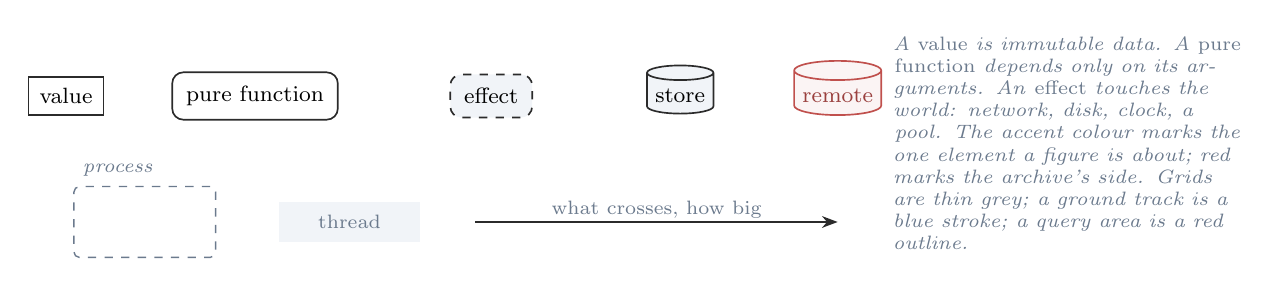
\begin{tikzpicture}[x=1mm,y=1mm]
  \node[val] (v) at (0,0) {value};
  \node[pure] (p) at (24,0) {pure function};
  \node[eff] (e) at (54,0) {effect};
  \node[store] (s) at (78,0) {store};
  \node[remote] (r) at (98,0) {remote};
  \node[proc, minimum width=18mm, minimum height=9mm] (pr) at (10,-16) {};
  \node[note, anchor=south west] at (pr.north west) {process};
  \node[lane, minimum width=18mm, minimum height=5mm] (ln) at (36,-16) {};
  \node[lbl] at (ln) {thread};
  \draw[flow] (52,-16) -- node[lblw, above] {what crosses, how big} (98,-16);
  \node[note, text width=44mm, anchor=west] at (104,-6)
    {A \emph{value} is immutable data. A \emph{pure function} depends only on its arguments. An \emph{effect}
     touches the world: network, disk, clock, a pool. The accent colour marks the one element a figure is about;
     red marks the archive's side. Grids are thin grey; a ground track is a blue stroke; a query area is a red
     outline.};
\end{tikzpicture}}
\caption{The figure grammar. Sharp corners are data; rounded corners are code; grey dashed code has side
effects; cylinders are stores, red when they belong to the archive. Arrows say what crosses and, where measured,
how much.}
\label{fig:legend}
\end{figure}

\tableofcontents

%=====================================================================================================================
\part{The data}
%=====================================================================================================================

\section{Along-track, non-gridded data}
\label{ch:alongtrack}

A laser altimeter measures the time of flight of a pulse from the instrument to the ground and back. Combined with
the instrument's position and pointing, each pulse gives one \emph{footprint}: a position on the ellipsoid, a
height, and a time. The instrument fires continuously while the platform moves, so the measurements form a
time-ordered sequence along a \emph{ground track}. Nothing about the sequence is a grid. Consecutive footprints are
metres to hundreds of metres apart along the track; the next track is kilometres away or, for a repeat pass, offset
by whatever the pointing achieved that day. The position of a measurement is \emph{data stored with it}, not
something implied by its place in an array.

That one property is the source of every difficulty this report is about. In a raster, the question ``which
elements lie inside this box'' is arithmetic on indices. In an along-track product, a point's position is known only
after the point has been read, so the question has no answer short of reading everything, unless someone has read
everything once and written the answer down.

\paragraph{The instruments.} Five sources of along-track data enter the system (Table~\ref{tab:missions},
Figure~\ref{fig:sampling}).

\begin{itemize}
\item \textbf{ICESat / GLAS} (2003--2009) carried a single-beam 1064\,nm altimeter firing at 40\,Hz, giving footprints
  of roughly 70\,m every $\sim$172\,m along track~\citep{schutz2005}. Early laser failures forced operation in
  33-day campaigns, three a year; the record is 19 campaigns, L1A through L2F, so coverage is intermittent in time by
  design. We use the GLAH06 land-elevation product, release 34~\citep{glah06v34}.
\item \textbf{Operation IceBridge / ATM} (2009--2019) flew the Airborne Topographic Mapper, a conically scanning
  lidar, on survey aircraft to bridge the gap between the two satellites~\citep{krabill2002}. The Level-2
  ``icessn'' product resamples the dense scan into platelets: a plane is fitted to blocks of points at regular
  intervals along and across the swath; each record is an 80\,m across-track nadir platelet, three or five outer
  platelets, and about half a second of flight~\citep{blatm2guide,ilatm2v2}. The result is a
  short, dense, irregular set of flight lines rather than an orbit.
\item \textbf{ICESat-2 / ATLAS} (2018--) splits a 532\,nm beam into three pairs; each pair is a strong and a weak beam
  (energy ratio about 4:1) 90\,m apart, and the pairs are 3.3\,km apart across track~\citep{markus2017}. The
  photon-counting detector records individual returned photons, about one every 0.7\,m along track. ATL03 is the
  geolocated photon product~\citep{neumann2019,atl03v7}; ATL06 fits 40\,m segments to the photons, posted every
  20\,m, and reports one land-ice height per segment~\citep{smith2019,atl06v7}. The 1\,387 reference ground tracks
  repeat every 91 days.
\item \textbf{GEDI} (2019--) is a lidar on the International Space Station: three lasers, one split into two
  coverage beams, dithered into eight ground tracks about 600\,m apart, each with 25\,m footprints every
  $\sim$60\,m~\citep{dubayah2020,gedigeometry}. The station's orbit confines it to $\pm$51.6$^\circ$, so it never
  sees an ice sheet; it enters the system for mountain glaciers and as a test that the design is not ice-specific.
  We use the L2A footprint product, version 3~\citep{gedi02av3}.
\item \textbf{The Summit traverse} is ground truth rather than altimetry: a kinematic GPS antenna on a sled towed
  monthly along a 15\,km transect west of Summit Station, Greenland, laid along ICESat-2 reference tracks 749 and
  879~\citep{is2tgpsss}. It has the along-track shape of an altimetry product and none of its scale.
\end{itemize}

\begin{table}[tbp]
\footnotesize
\wide{\begin{tabular}{@{}lllllll@{}}
\toprule
source & product & years & footprint & along-track & beams or tracks & latitude \\
\midrule
ICESat GLAS & GLAH06 r34 & 2003--09 & $\sim$70\,m & $\sim$172\,m & 1 & $\pm$86$^\circ$ \\
IceBridge ATM & ILATM2 v2 & 2009--19 & 80\,m platelet & $\sim$0.5\,s of flight & nadir + 3--5 outer & 60--90$^\circ$N, 53--90$^\circ$S \\
ICESat-2 ATLAS & ATL03 v7 & 2018-- & $\sim$17\,m & $\sim$0.7\,m (photons) & 3 pairs, strong/weak & $\pm$88$^\circ$ \\
ICESat-2 ATLAS & ATL06 v7 & 2018-- & 40\,m segment & 20\,m posting & 3 pairs, strong/weak & $\pm$88$^\circ$ \\
GEDI & GEDI02\_A v3 & 2019-- & 25\,m & $\sim$60\,m & 8 tracks, full/coverage & $\pm$51.6$^\circ$ \\
Summit GPS & IS2TGPSSS v1 & 2006-- & point & continuous & 1 transect & Summit only \\
\bottomrule
\end{tabular}}
\caption{The along-track sources in the system. The latitude column is the declared footprint the system uses to
decide whether a collection can have data over an area at all; the years are the default search windows.}
\label{tab:missions}
\end{table}

\begin{figure}[tbp]
\wide{%
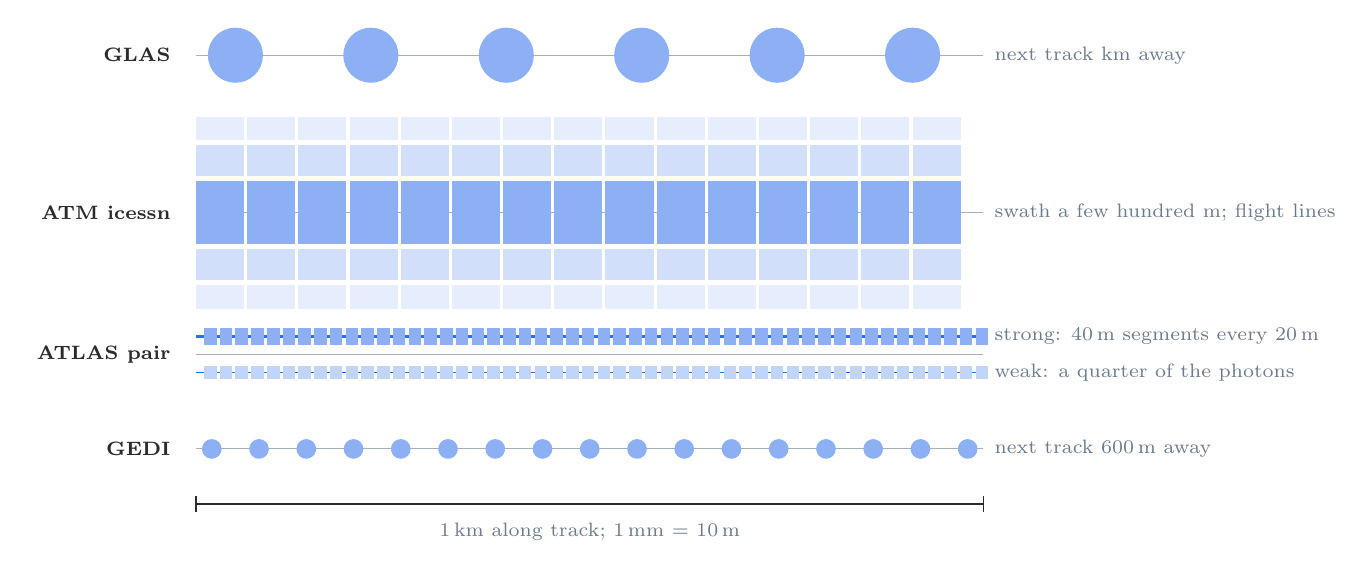
\begin{tikzpicture}[x=1mm,y=1mm]
  % scale: 1 mm = 10 m along track; each panel shows one kilometre of track
  \foreach \yy/\lab in {56/GLAS, 36/ATM icessn, 18/ATLAS pair, 6/GEDI} {
    \node[hdr, anchor=east] at (-2,\yy) {\lab};
    \draw[grid] (0,\yy) -- (100,\yy);
  }
  % GLAS: 70 m footprints every 172 m
  \foreach \x in {5,22.2,39.4,56.6,73.8,91} { \fill[foot] (\x,56) circle (3.5); }
  % ATM: nadir platelet 80 m across (8 mm tall), ~65 m along (6.5 mm); outer platelets dimmer, +-20 mm
  \foreach \x in {0,6.5,...,93.5} {
    \fill[idxblue!55] (\x,32) rectangle (\x+6.1,40);
    \fill[idxblue!22] (\x,40.6) rectangle (\x+6.1,44.6); \fill[idxblue!22] (\x,27.4) rectangle (\x+6.1,31.4);
    \fill[idxblue!12] (\x,45.2) rectangle (\x+6.1,48.2); \fill[idxblue!12] (\x,23.8) rectangle (\x+6.1,26.8);
  }
  % ATLAS: strong (y=22.3) and weak (y=17.7) 90 m apart -> 9 mm (shown at 4.6 mm from the axis each side)
  \draw[track] (0,20.3) -- (100,20.3); \draw[track, line width=0.4pt] (0,15.7) -- (100,15.7);
  \foreach \x in {1,3,...,99} { \fill[idxblue!55] (\x,19.2) rectangle (\x+1.6,21.4); }
  \foreach \x in {1,3,...,99} { \fill[idxblue!30] (\x,14.9) rectangle (\x+1.6,16.5); }
  \node[lbl, anchor=west] at (101,20.3) {strong: 40\,m segments every 20\,m};
  \node[lbl, anchor=west] at (101,15.7) {weak: a quarter of the photons};
  % GEDI: 25 m footprints every 60 m; a second track would be 600 m away
  \foreach \x in {2,8,...,98} { \fill[foot] (\x,6) circle (1.25); }
  \node[lbl, anchor=west] at (101,6) {next track 600\,m away};
  \node[lbl, anchor=west] at (101,56) {next track km away};
  \node[lbl, anchor=west] at (101,36) {swath a few hundred m; flight lines};
  \draw[draw=ink, line width=0.5pt] (0,-1) -- (100,-1); \draw[draw=ink, line width=0.5pt] (0,-2) -- (0,0); \draw[draw=ink, line width=0.5pt] (100,-2) -- (100,0);
  \node[lbl] at (50,-4.5) {1\,km along track; 1\,mm = 10\,m};
\end{tikzpicture}}
\caption{One kilometre of each instrument's sampling at one scale. The products differ by three orders of
magnitude in along-track density and by as much across track, but all of them are sequences of positioned
measurements along a line, and none of them is a grid.}
\label{fig:sampling}
\end{figure}

\paragraph{What they share.} Every source delivers positions, heights and times as parallel arrays in time order,
with quality indicators alongside; every source is sparse across track and continuous along it; and every source
has holes. GLAS returns from cloud tops sit kilometres above the surface; its own cloud flag is set on 99.9\,\% of
shots and so distinguishes nothing, while about 3\,\% of shots are gross cloud returns. ATLAS loses the surface
under thick cloud and over wet firn the 532\,nm signal penetrates the snow. GEDI's accuracy degrades with slope.
Fill values mark where an algorithm declined to report: GLAS uses $1.798\times10^{308}$ where a reader expects NaN,
ATL06 uses a large positive float. Any system that indexes these data must therefore record where points \emph{are}
rather than where the track \emph{was}, and must be prepared for a granule that crosses an area to contribute
nothing to it.

\section{Logical organisation: the granule and the product}
\label{ch:logical}

The archive's unit is the \emph{granule}: one file, catalogued once, with a footprint and a time range. What a
granule contains is a product decision, and it differs by mission (Figure~\ref{fig:regions}).

\begin{itemize}
\item An ICESat-2 orbit is cut into 14 \emph{regions} by lines of latitude at 27$^\circ$, 59.5$^\circ$ and
  80$^\circ$ in each hemisphere, ascending and descending halves separately~\citep{atl06v7}. An ATL03 or ATL06
  granule is one reference ground track (RGT), one cycle, one region: for Greenland, regions 03 and 05
  (59.5--80$^\circ$N, ascending and descending) and 04 (the arc above 80$^\circ$N). Its name carries the start
  time, RGT, cycle, region, version and release:
  \code{ATL06\_20181014050737\_02380104\_007\_01.h5} is RGT 0238, cycle 01, region 04.
\item A GLAH06 granule is a long orbit arc, pole to pole; the file name has no date, so the first shot's time is
  the only clock.
\item An ILATM2 granule is a few minutes of one flight (about four minutes in the deployed index); a flight
  day yields dozens, a campaign thousands. Its name carries the date and the start time of the slice.
\item A GEDI L2A granule is a quarter orbit, about fifteen minutes and $\sim$170\,000 shots per beam, named by
  day-of-year, orbit and track.
\item A traverse survey is one CSV file per monthly survey.
\end{itemize}

\begin{figure}[tbp]
\wide{%
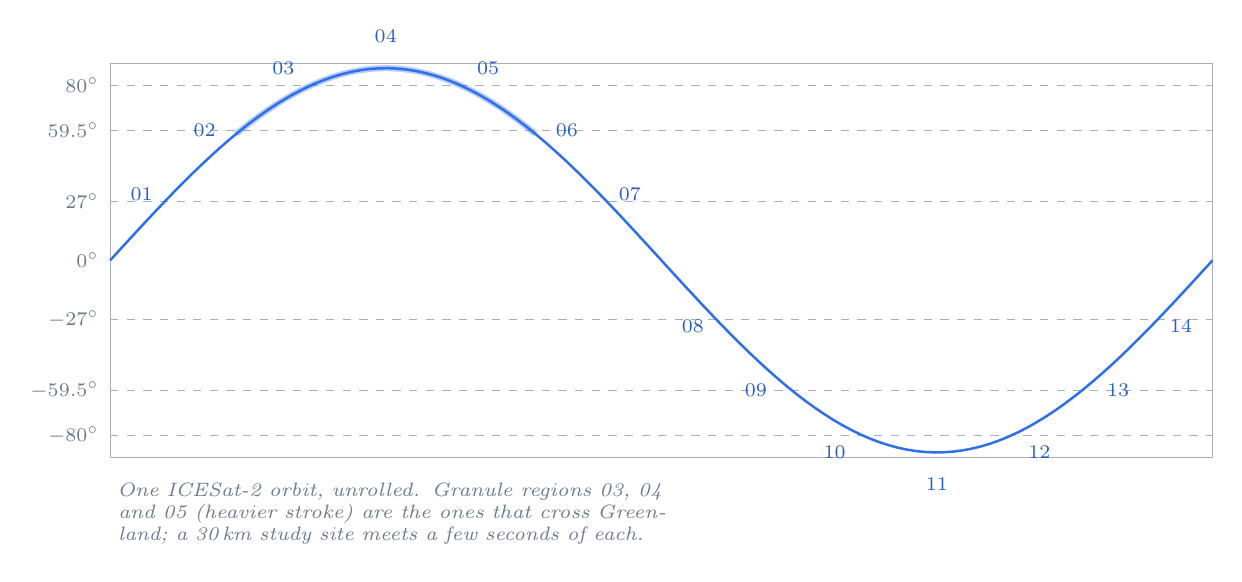
\begin{tikzpicture}[x=1mm,y=1mm]
  % lon/lat frame: 140 mm = 360 deg lon, 50 mm = 180 deg lat
  \draw[grid] (0,-25) rectangle (140,25);
  \foreach \la/\t in {27/27, -27/-27, 59.5/59.5, -59.5/-59.5, 80/80, -80/-80} {
    \draw[grid, dashed] (0,{\la*50/180}) -- (140,{\la*50/180});
    \node[lbl, anchor=east] at (-1,{\la*50/180}) {$\t^\circ$};
  }
  \node[lbl, anchor=east] at (-1,0) {0$^\circ$};
  % one orbit: ground track of a 92 deg inclination orbit as a sinusoid-like curve (schematic), ascending then descending
  \draw[track] plot[domain=0:140, samples=120] (\x, {24.4*sin(deg(\x/140*2*pi))});
  % region boundaries along the curve: mark where the curve crosses the latitude lines on the ascending half
  % labels of regions along the ascending and descending halves (schematic positions)
  \foreach \x/\n in {4/01, 12/02, 22/03, 35/04, 48/05, 58/06, 66/07, 74/08, 82/09, 92/10, 105/11, 118/12, 128/13, 136/14} {
    \node[lbl, text=idxblue!85!black] at (\x, {24.4*sin(deg(\x/140*2*pi)) + (\x<70 ? 4 : -4)}) {\n};
  }
  % Greenland regions highlighted
  \draw[draw=idxblue, line width=2.2pt, opacity=0.35] plot[domain=16:54, samples=60] (\x, {24.4*sin(deg(\x/140*2*pi))});
  \node[note, anchor=north west, text width=70mm] at (0,-27) {One ICESat-2 orbit, unrolled. Granule regions 03,
    04 and 05 (heavier stroke) are the ones that cross Greenland; a 30\,km study site meets a few seconds of each.};
\end{tikzpicture}}
\caption{The granule is a product decision, not a geographic one. An ICESat-2 granule is one fourteenth of an
orbit cut by latitude; a GLAS granule is a longer arc; an IceBridge granule is a few minutes of a flight. In every
case the granule is hundreds to thousands of kilometres long and a study site needs a sliver of it.}
\label{fig:regions}
\end{figure}

\paragraph{Inside a granule.} The HDF5 products are trees of groups that hold datasets. ATL03 and ATL06 have one
group per beam (\code{gt1l} \ldots\ \code{gt3r}); which of the pair is the strong beam depends on the spacecraft's
yaw orientation, a scalar stored once per file, and a yaw flip in progress leaves the question unanswerable for
that granule. Within a beam, ATL06's \code{land\_ice\_segments} holds parallel arrays, one element per segment:
latitude, longitude, height, time, a quality summary, and many more we do not read. ATL03's \code{heights} group
holds one element per \emph{photon}, and its \code{geolocation} group holds one element per 20\,m
\emph{segment}, with each segment recording the index of its first photon and its photon count; a photon's
position is thus available both directly and, far more cheaply, through its segment. GLAH06 has no beams: one
\code{Data\_40HZ} group with one element per shot. GEDI has eight beam groups, each with per-shot arrays whose
elevation is the lowest detected mode. The text products are one record per line: ILATM2 has eleven
comma-separated fields per platelet (time of day, position, elevation, slopes, fit RMS, point counts, a distance,
and the across-track \emph{track} number, zero for nadir); the traverse file has twelve (position, antenna height,
time, satellite geometry, and 95\,\% uncertainties).

\paragraph{Time is encoded five ways.} ATLAS stores seconds since an epoch that is itself stored in the file, in GPS
seconds since 1980, which differ from UTC by 18 leap seconds. GLAS stores seconds since J2000, noon on
2000-01-01. ILATM2 stores seconds of day, with the day in the file name. The traverse stores decimal hours with
day-of-year and year in separate columns. GEDI's time we do not read: the date comes from its file name. A system
that wants a temporal predicate has to normalise all five before it can compare anything, and the cheapest reliable
clock is usually the file name.

\paragraph{Frames and heights.} Heights are above an ellipsoid, but not the same one in the same frame. ATL06 is
WGS84 in ITRF2014, with ocean tide and dynamic atmosphere corrections deliberately not applied. GLAH06 reports
heights above the TOPEX/Poseidon ellipsoid in ITRF2008; the published conversion to WGS84 subtracts about 0.70\,m.
ILATM2's frame is whichever ITRF realisation the campaign used, read per granule from the header. The traverse is
GRS80 in ITRF2020, and its surface height is the antenna height minus a sled geometry that changed in 2014. None of
this concerns the index, which records where bytes are; all of it concerns the analyses that read the lake, which is
why the lake stores each source's native height and the conversion lives in the source's descriptor
(Chapter~\ref{ch:descriptor}).

\paragraph{Quality.} Each product has its own notion: ATL06's quality summary (zero is good); ATL03's per-photon
signal confidence, a five-column array of which one column is the land-ice classification; GLAH06's elevation-use
and saturation-correction flags; ILATM2's plane-fit RMS; GEDI's quality and degrade flags (which together keep
41\,\% of shots over Langtang); the traverse's height uncertainty. These are filters on \emph{points}, applied after
retrieval, and the only one the design asks the index to know about is the one that changes which bytes are needed:
none of them do. Table~\ref{tab:logical} collects the per-collection facts the rest of the report relies on.

\begin{table}[tbp]
\footnotesize
\wide{\begin{tabular}{@{}llp{30mm}p{27mm}p{24mm}p{28mm}@{}}
\toprule
collection & granule is & positions & height & time & quality \\
\midrule
ATL03 & RGT$\times$cycle$\times$region & \code{lat\_ph}, \code{lon\_ph} per photon; segments carry a reference photon & \code{h\_ph} & \code{delta\_time} + SDP epoch (GPS) & \code{signal\_conf\_ph[:,3]} $\ge$ 3 \\
ATL06 & RGT$\times$cycle$\times$region & \code{latitude}, \code{longitude} per segment & \code{h\_li} & \code{delta\_time} + SDP epoch (GPS) & \code{atl06\_quality\_summary} = 0 \\
GLAH06 & orbit arc & \code{d\_lat}, \code{d\_lon} (0--360) per shot & \code{d\_elev} + sat.\ corr.\ $-$ T/P offset & \code{DS\_UTCTime\_40} (J2000) & \code{elev\_use\_flg} = 0, \code{sat\_corr\_flg} $\le$ 2 \\
GEDI L2A & quarter orbit & \code{lat/lon\_lowestmode} per shot & \code{elev\_lowestmode} & file name (day of year) & \code{quality\_flag} = 1, \code{degrade\_flag} = 0 \\
ILATM2 & minutes of flight & columns 2--3 per platelet (0--360) & column 4 & seconds of day + file date & \code{track} = 0, RMS $<$ 50\,cm \\
IS2TGPSSS & one survey & columns 1--2 per fix & antenna HAE $-$ sled + track depth & decimal hour, DOY, year & \code{SDHGT\_95} $<$ 0.5\,m \\
\bottomrule
\end{tabular}}
\caption{The logical facts per collection. Everything in this table becomes a field of the collection descriptor
in Part~\ref{part:framework}; nothing in it is known to the shared pipeline.}
\label{tab:logical}
\end{table}

\section{Physical organisation: how the bytes lie}
\label{ch:physical}

Four of the six collections are HDF5 files; two are CSV text. The design needs only a small part of HDF5, but that
part has to be exact, because the system will address bytes inside files it never opens again.

\paragraph{Chunks.} An HDF5 dataset is stored in \emph{chunks}: fixed-size pieces of the array, each compressed
on its own (gzip, usually after a byte-shuffle filter that groups the bytes of each element's position to compress
better) and written wherever the file had room at the time~\citep{hdf5format}. A B-tree per dataset maps chunk
number to (offset, size) in the file. Reading element $i$ means finding chunk $i\,\mathrm{div}\,C$ in that tree,
fetching its bytes, decompressing them, and taking element $i \bmod C$. The chunk is therefore three things at
once: the unit of compression, the unit of I/O, and the smallest thing a byte-range request can usefully ask for
(Figure~\ref{fig:chunkmap}).
\begin{figure}[tbp]
\wide{%
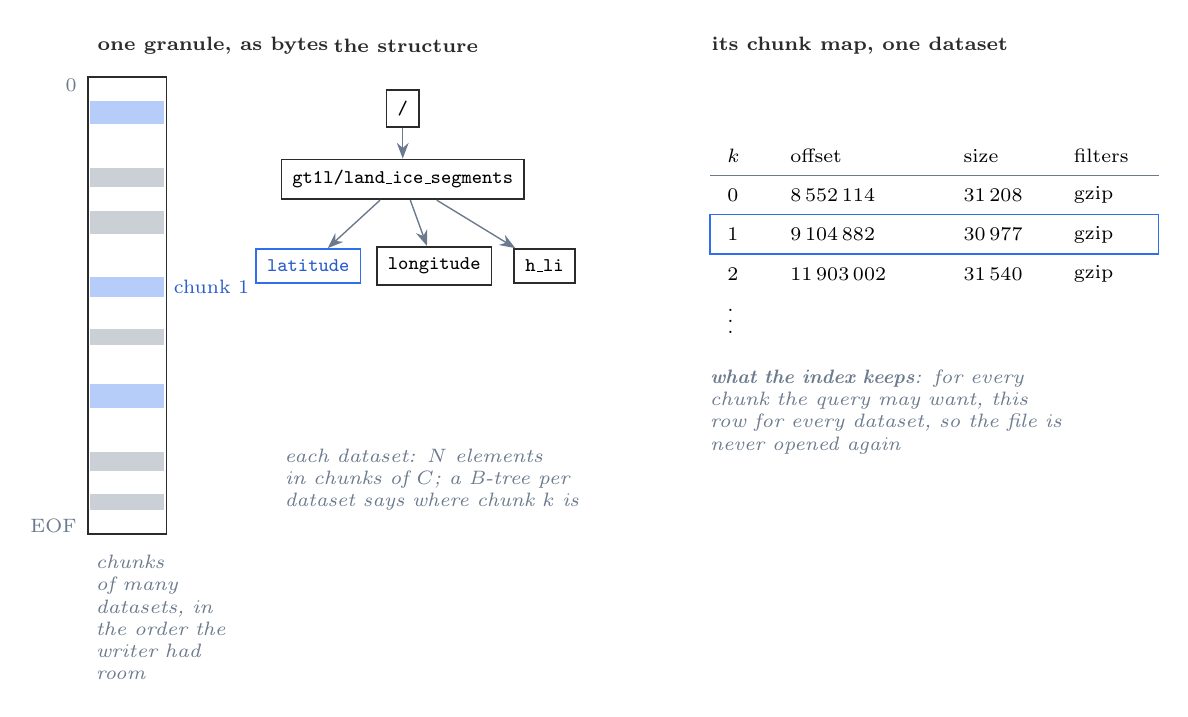
\begin{tikzpicture}[x=1mm,y=1mm]
  % the file as a byte column
  \node[hdr] at (0,62) {one granule, as bytes};
  \draw[draw=ink, line width=0.6pt] (0,0) rectangle (10,58);
  \foreach \y/\h/\c in {52/3/idxblue, 44/2.5/soft, 38/3/soft, 30/2.6/idxblue, 24/2/soft, 16/3/idxblue, 8/2.4/soft, 3/2/soft}
    {\fill[\c!35] (0.3,\y) rectangle (9.7,\y+\h);}
  \node[lbl, anchor=east] at (-1,57) {0};
  \node[lbl, anchor=east] at (-1,1) {EOF};
  \node[note, text width=18mm, anchor=north west] at (0,-1.5) {chunks of many datasets, in the order the writer
    had room};
  % the tree
  \node[hdr] at (30,62) {the structure};
  \node[val, font=\scriptsize] (root) at (40,54) {\code{/}};
  \node[val, font=\scriptsize] (g) at (40,45) {\code{gt1l/land\_ice\_segments}};
  \node[val, font=\scriptsize, acc] (lat) at (28,34) {\code{latitude}};
  \node[val, font=\scriptsize] (lon) at (44,34) {\code{longitude}};
  \node[val, font=\scriptsize] (h) at (58,34) {\code{h\_li}};
  \draw[flowsoft] (root) -- (g); \draw[flowsoft] (g) -- (lat); \draw[flowsoft] (g) -- (lon); \draw[flowsoft] (g) -- (h);
  \node[note, text width=40mm, anchor=north west] at (24,12) {each dataset: $N$ elements in chunks of $C$;
    a B-tree per dataset says where chunk $k$ is};
  % the chunk map
  \node[hdr] at (78,62) {its chunk map, one dataset};
  \foreach \r/\k/\o/\z/\f in {0/$k$/offset/size/filters, 1/0/8\,552\,114/31\,208/gzip, 2/1/9\,104\,882/30\,977/gzip, 3/2/11\,903\,002/31\,540/gzip, 4/$\vdots$//{}/{}} {
    \node[font=\scriptsize, anchor=west] at (80,{48-5*\r}) {\k};
    \node[font=\scriptsize, anchor=west] at (88,{48-5*\r}) {\o};
    \node[font=\scriptsize, anchor=west] at (110,{48-5*\r}) {\z};
    \node[font=\scriptsize, anchor=west] at (124,{48-5*\r}) {\f};
  }
  \draw[draw=soft, line width=0.4pt] (79,45.5) -- (136,45.5);
  % connect chunk 1 to the byte column
  \node[lbl, anchor=west, text=idxblue!85!black] at (10.5,31.3) {chunk 1};
  \draw[draw=idxblue, line width=0.5pt] (79,40.5) rectangle (136,35.5);
  \node[note, text width=46mm, anchor=north west] at (78,22) {\textbf{what the index keeps}: for every chunk the
    query may want, this row for every dataset, so the file is never opened again};
\end{tikzpicture}}
\caption{A granule's bytes, its structure, and the chunk map that connects them. The index is the chunk map,
reorganised by where on the Earth each chunk's points fall.}
\label{fig:chunkmap}
\end{figure}

The chunk map (Figure~\ref{fig:chunkmap}) is the only thing the query needs from the file's structure. Walking the
tree to obtain it is the expensive part of a build; Chapter~\ref{ch:readgranule} is about making that walk cheap.
Decoding a chunk is the cheap, pure part: inflate, undo the shuffle, reinterpret as the dtype.\side{Decoding is
validated byte-identical against the reference HDF5 library on real chunks; it needs no HDF5 code at query time.}

\paragraph{Three layouts.} The collections differ in how their datasets are chunked, and that difference decides
what a row of the index can mean (Figure~\ref{fig:layouts}).

\begin{figure}[tbp]
\wide{%
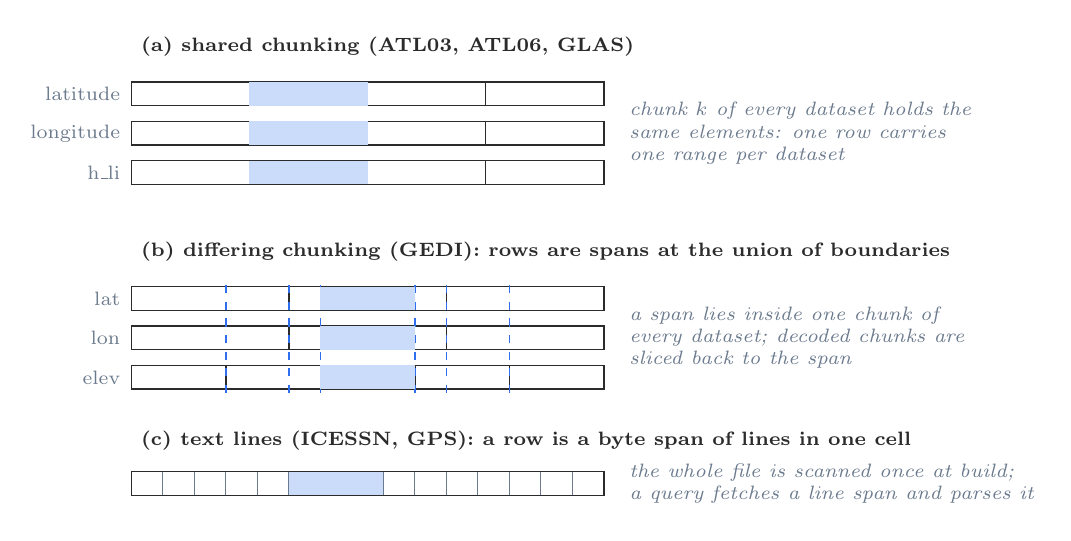
\begin{tikzpicture}[x=1mm,y=1mm]
  % (a) shared
  \node[hdr] at (0,30) {(a) shared chunking (ATL03, ATL06, GLAS)};
  \foreach \r/\n in {0/latitude, 1/longitude, 2/h\_li} {
    \node[lbl, anchor=east] at (-1,{24-5*\r}) {\n};
    \draw[draw=ink, line width=0.5pt] (0,{22.5-5*\r}) rectangle (60,{25.5-5*\r});
    \foreach \x in {15,30,45} \draw[draw=ink, line width=0.5pt] (\x,{22.5-5*\r}) -- (\x,{25.5-5*\r});
  }
  \fill[idxblue!25] (15,22.5) rectangle (30,25.5); \fill[idxblue!25] (15,17.5) rectangle (30,20.5); \fill[idxblue!25] (15,12.5) rectangle (30,15.5);
  \node[note, anchor=west] at (62,19) {chunk $k$ of every dataset holds the\\same elements: one row carries\\one range per dataset};
  % (b) spans
  \node[hdr] at (0,4) {(b) differing chunking (GEDI): rows are spans at the union of boundaries};
  \foreach \r/\n/\c in {0/lat/20, 1/lon/20, 2/elev/12} {
    \node[lbl, anchor=east] at (-1,{-2-5*\r}) {\n};
    \draw[draw=ink, line width=0.5pt] (0,{-3.5-5*\r}) rectangle (60,{-0.5-5*\r});
    \foreach \x in {\c,...,59} {\pgfmathparse{int(mod(\x,\c))}\ifnum\pgfmathresult=0 \draw[draw=ink, line width=0.5pt] (\x,{-3.5-5*\r}) -- (\x,{-0.5-5*\r});\fi}
  }
  \foreach \x in {12,20,24,36,40,48} \draw[draw=idxblue, dashed, line width=0.5pt] (\x,-14) -- (\x,0);
  \fill[idxblue!25] (24,-3.5) rectangle (36,-0.5); \fill[idxblue!25] (24,-8.5) rectangle (36,-5.5); \fill[idxblue!25] (24,-13.5) rectangle (36,-10.5);
  \node[note, anchor=west] at (62,-7) {a span lies inside one chunk of\\every dataset; decoded chunks are\\sliced back to the span};
  % (c) lines
  \node[hdr] at (0,-20) {(c) text lines (ICESSN, GPS): a row is a byte span of lines in one cell};
  \draw[draw=ink, line width=0.5pt] (0,-27) rectangle (60,-24);
  \foreach \x in {4,8,...,56} \draw[draw=soft, line width=0.3pt] (\x,-27) -- (\x,-24);
  \fill[idxblue!25] (20,-27) rectangle (32,-24);
  \node[note, anchor=west] at (62,-25.5) {the whole file is scanned once at build;\\a query fetches a line span and parses it};
\end{tikzpicture}}
\caption{Three storage layouts, one index shape. In each case a row names a contiguous element interval and the
byte ranges that hold it, so the query reads ranges and slices without knowing which layout produced the row.}
\label{fig:layouts}
\end{figure}

For the ICESat products and GLAS, every dataset of a group is chunked identically (10{,}000 segments per chunk in
ATL06, 100{,}000 photons in ATL03), so chunk $k$ of the latitude dataset covers the same elements as chunk $k$ of
the height dataset, and one row can carry one byte range per dataset. GEDI chunks its datasets differently; the
design cuts the element axis at the union of every dataset's chunk boundaries, so each resulting \emph{span} lies
inside exactly one chunk of every dataset and the row again carries one range per dataset, plus the offset of the
span inside each chunk. The text collections have no chunks at all: the build scans the whole file once and a row
is the byte span of the lines that fall in one cell.

\paragraph{ATL03's indirection.} The photon product adds one twist that matters later. Photons are stored by
time, and their positions are stored twice: every photon has its own latitude and longitude, and every 20\,m
\emph{segment} has a reference photon and a count. A build cannot afford to read a billion photon positions, so it
reads the segment positions and maps each segment's photon range (\code{ph\_index\_beg}, \code{segment\_ph\_cnt})
onto chunks. A chunk of 100{,}000 photons is thus located by the few hundred segments that cover it.

\paragraph{One shape, six sources.} Table~\ref{tab:collections} is the whole of what differs in \emph{layout};
everything else is shared. Read with Tables~\ref{tab:logical} and \ref{tab:physical} it is, almost verbatim, the
collection descriptor of Chapter~\ref{ch:descriptor}.

\begin{table}[tbp]
\footnotesize
\wide{\begin{tabular}{@{}lllp{30mm}p{36mm}@{}}
\toprule
collection & product & layout & position source & group structure \\
\midrule
ATL03 & ICESat-2 photons & shared chunks & segment reference photons & 6 beams; strong/weak \\
ATL06 & ICESat-2 land ice & shared chunks & per segment & 6 beams; strong/weak \\
GLAS & ICESat GLAH06 & shared chunks & per shot & one group \\
GEDI & GEDI L2A & spans & per shot & 8 beams; full/coverage power \\
ICESSN & IceBridge ATM L2 & text lines & per platelet line & none \\
GPS & Summit traverse & text lines & per fix line & none; sled geometry from a metadata file \\
\bottomrule
\end{tabular}}
\caption{What differs between collections in layout. Each difference is a value or a small function in Part~\ref{part:framework}.}
\label{tab:collections}
\end{table}


\paragraph{Where the chunks lie.} Nothing requires chunk $k$ of one dataset to sit near chunk $k$ of another, or
near chunk $k+1$ of itself, and the writers do not try. In the example ATL06 granule the five datasets' chunks for
one 10\,000-segment stretch of one beam are five ranges of 91 to 2\,866 bytes that happen to lie within 8\,577
bytes of each other, so one 8.6\,kB request fetches the lot; in an ATL03 granule one chunk's five ranges can be
3.28\,GB apart. The compressed size of a chunk also varies with content: a quality-flag chunk of 10\,000 one-byte
values gzips to 91 bytes, a latitude chunk of 10\,000 doubles to 2.7\,kB. The index must therefore record, per
chunk, per dataset, an exact (offset, size), and the fetcher must be prepared to coalesce neighbours and to leave
distant ranges as separate requests.

\paragraph{How much there is.} Table~\ref{tab:physical} gives the chunk lengths and granule sizes measured on the
deployed instance. Three numbers set the scale of everything that follows. An ATL06 granule over Greenland is
64--104\,MB (quartiles 72 / 88 / 96\,MB from the catalogue's own size field) and holds about five chunks of 10\,000
segments per beam inside the region; its segments are 20\,m apart, so one chunk is about 200\,km of track. An ATL03
granule is 0.2--6.7\,GB (quartiles 0.95 / 1.4 / 2.7\,GB over Summit) and holds about a hundred chunks of 100\,000
photons per beam. A GLAH06 granule is 3--5\,MB and an ILATM2 granule 0.1--0.5\,MB. The regional indexes on the
deployed machine cover 33\,484 ATL06 granules, 48\,838 ATL03 granules, 4\,799 GLAH06 arcs and 33\,811 ILATM2
slices.\landed{the chunk map is read by \code{index.\_chunk\_manifest} through h5py's \code{chunk\_iter}; GEDI's
span cutting is \code{index\_gedi.chunk\_spans}; the line parsers are \code{index\_icessn.\_parse\_fields} and
\code{index\_gpstruth}; sizes from \code{scripts/measure\_search\_modes.py} and \code{bench\_build\_io.py}.}

\begin{table}[tbp]
\footnotesize
\wide{\begin{tabular}{@{}lllllr@{}}
\toprule
collection & format & chunk (elements) & filters & granule size & indexed \\
\midrule
ATL03 & HDF5 & 100\,000 photons, shared by the group & gzip (+ shuffle) & 0.2--6.7\,GB; Q 0.95 / 1.4 / 2.7\,GB & 48\,838 \\
ATL06 & HDF5 & 10\,000 segments, shared by the group & gzip (+ shuffle) & 64--104\,MB; Q 72 / 88 / 96\,MB & 33\,484 \\
GLAH06 & HDF5 & shared, one group & gzip & 3--5\,MB; Q 3.3 / 3.9 / 4.2\,MB & 4\,799 \\
GEDI L2A & HDF5 & 2\,608 / 5\,216 / 10\,432 / 100\,000 per dataset & gzip & $\sim$100\,MB & Langtang only \\
ILATM2 & CSV & lines & none & 0.1--0.5\,MB & 33\,811 \\
IS2TGPSSS & CSV & lines & none & 0.1--1\,MB & 272 \\
\bottomrule
\end{tabular}}
\caption{The physical facts per collection. ``Q'' are size quartiles from the catalogue's size field over the Summit
box (Langtang for GEDI). GEDI's four chunk lengths differ by 38$\times$ between datasets, which is why its index rows
are spans rather than chunks.}
\label{tab:physical}
\end{table}

%=====================================================================================================================
\clearpage
\part{The problem}
%=====================================================================================================================

\section{A canonical set of queries}
\label{ch:queries}

Before designing anything we fix what the system is asked. The questions come from two places: the tools the
deployed server exposes to an analyst or a language model, and the science questions the project set out to answer
(the inter-mission elevation-change comparison, its feasibility over a candidate site, the long record at a
glacier). Reduced to their shape, every one is a conjunction of four kinds of constraint.

\begin{description}\setlength{\itemsep}{2pt}
\item[Area.] A named region; a rectangle in longitude and latitude; a polygon; a point and a radius; or a grid
  cell with a resolution. The deployed regions are 0.1--3$^\circ$ across (Table~\ref{tab:regions}, Figure~\ref{fig:areaforms}); a cell at the
  analysis resolution is about half a kilometre.
\item[Time.] A window of dates; the whole record; or a mission-specific bucket (a GLAS laser campaign, an ICESat-2
  cycle, an IceBridge season). Every window is finally compared with a clock encoded five ways
  (Chapter~\ref{ch:logical}).
\item[Filters.] Per-mission quality predicates (Table~\ref{tab:logical}); which beams or beam groups (strong only,
  all six; full-power only); a confidence threshold for photons; a slope ceiling for GEDI.
\item[Aggregation.] None, the points themselves. Per-cell statistics: counts, passes, days, years, the height
  median and its spread. Co-located pairs between two sources with a difference and its robust spread. A per-cell
  time series with window medians and a trend.
\end{description}

\begin{table}[tbp]
\footnotesize
\wide{\begin{tabular}{@{}llp{64mm}@{}}
\toprule
region & bbox (W, S, E, N) & role \\
\midrule
summit & $-39.5, 72.4, -37.5, 72.8$ & cleanest interior; the ground-truth neighbourhood \\
summit\_traverse & $-38.586, 72.579, -38.474, 72.648$ & the 15\,km GPS transect itself \\
egig\_west\_flank & $-45.0, 69.8, -43.0, 70.2$ & default demo region; EGIG line, central-west flank \\
k\_transect\_upstream & $-48.5, 66.9, -46.5, 67.3$ & upstream of the ablation zone \\
jakobshavn\_margin & $-51.0, 69.0, -49.0, 69.4$ & fast ice; the long-record showcase \\
ne\_flank\_upstream\_negis & $-32.0, 75.5, -29.0, 76.0$ & NE interior flank \\
langtang & $85.35, 28.20, 85.62, 28.38$ & High Mountain Asia; the GEDI site \\
\bottomrule
\end{tabular}}
\caption{The named areas the system is asked about. All but Langtang are on the Greenland ice sheet; the traverse
box is 0.11$^\circ$ by 0.07$^\circ$, the others 2--3$^\circ$ by 0.4--0.5$^\circ$.}
\label{tab:regions}
\end{table}

Six prototypes cover what is asked today (Table~\ref{tab:queries}). They are written as specifications, not as
procedures, because the design's first move will be to treat a query as a \emph{value} that the system plans
against rather than a sequence of calls.

\begin{description}\setlength{\itemsep}{2pt}
\item[Q1 Points.] Every point of the selected sources inside an area over a window, with the per-source quality
  filter applied and the beam group chosen; returned as a table and drawn. This is the primitive; every other
  query is Q1 followed by arithmetic.
\item[Q2 Coverage.] For an area, per source: how many passes, distinct days and distinct years touch each cell at a
  coarse resolution, and whether a long record exists. Answered before any data are fetched; it decides whether a
  site is worth the fetch.
\item[Q3 Elevation change between epochs.] Points of two sources (GLAS and ATL06, say) inside an area, paired within
  35\,m, differenced after frame and epoch corrections, summarised as a median and a robust spread. Needs Q1 for two
  sources and a co-location.
\item[Q4 Per-cell time series.] For each cell at resolution 8 (about 530\,m across) in an area: all points of all
  sources, binned into windows of a year, a fixed-effects surface removing the within-cell slope, window medians,
  and a least-squares trend with a confidence that ranks cells. Needs Q1 for every source and a lot of per-cell
  arithmetic.
\item[Q5 Profile.] Points along a line (a transect, a flight line, a lake shoreline) at full resolution, per pass,
  for a water-level or a slope question. A thin polygon in Q1's terms, with the aggregation per pass.
\item[Q6 Triage.] ``Is site $X$ feasible?'' Q2 for every source plus the declared footprints: a source that never
  flew there must say so rather than report an empty index.
\end{description}

\begin{table}[tbp]
\footnotesize
\wide{\begin{tabular}{@{}lllll@{}}
\toprule
query & area & time & filters & aggregation \\
\midrule
Q1 points & region / bbox / polygon & window or all & quality, beam group, confidence & none \\
Q2 coverage & point + radius, or bbox & all & none & passes, days, years per coarse cell \\
Q3 change & bbox or polygon & two windows & quality; both sources & co-located pairs, median, MAD \\
Q4 time series & bbox, then res-8 cells & yearly windows & quality; reference source & plane fit, window medians, trend \\
Q5 profile & thin polygon / line & window or all & quality, confidence (lower for water) & per pass \\
Q6 triage & point + radius & all & footprints & Q2 per source, with ``never flew here'' \\
\bottomrule
\end{tabular}}
\caption{The six canonical queries as rows of the constraint algebra. Q1 is the primitive: every other row is Q1
over one or more sources followed by arithmetic on the points.}
\label{tab:queries}
\end{table}

\begin{figure}[tbp]
\wide{%
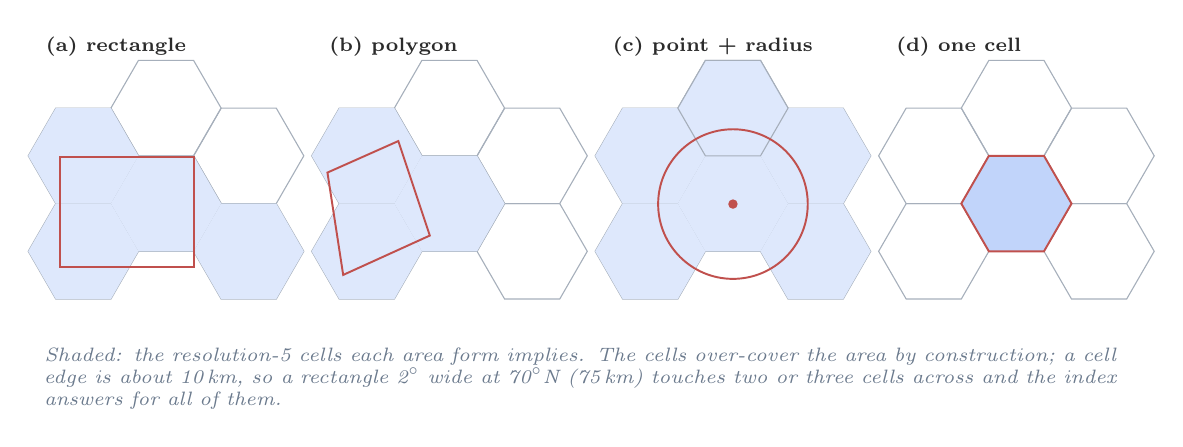
\begin{tikzpicture}[x=1mm,y=1mm]
  % four area forms over the same patch of res-5 cells (hex grid, r=7mm ~ 10 km edge)
  \foreach \px/\lab in {0/(a) rectangle, 36/(b) polygon, 72/(c) point + radius, 108/(d) one cell} {
    \begin{scope}[shift={(\px,0)}]
      \node[hdr] at (-6,26) {\lab};
      \foreach \i in {0,2} { \foreach \j in {0,1} { \draw[grid] \hexp{10.5*\i}{12.124*\j}{7}{0}; } }
      \foreach \i in {1} { \foreach \j in {0,1} { \draw[grid] \hexp{10.5*\i}{12.124*\j+6.062}{7}{0}; } }
    \end{scope}
  }
  % (a) rectangle: touches 4 cells
  \fill[idxblue!16] \hexp{0}{0}{7}{0}; \fill[idxblue!16] \hexp{10.5}{6.062}{7}{0}; \fill[idxblue!16] \hexp{21}{0}{7}{0}; \fill[idxblue!16] \hexp{0}{12.124}{7}{0};
  \draw[box] (-3,-2) rectangle (14,12);
  % (b) polygon
  \fill[idxblue!16] \hexp{36}{0}{7}{0}; \fill[idxblue!16] \hexp{46.5}{6.062}{7}{0}; \fill[idxblue!16] \hexp{36}{12.124}{7}{0};
  \draw[box] (33,-3) -- (44,2) -- (40,14) -- (31,10) -- cycle;
  % (c) disk
  \fill[idxblue!16] \hexp{72}{0}{7}{0}; \fill[idxblue!16] \hexp{82.5}{6.062}{7}{0}; \fill[idxblue!16] \hexp{72}{12.124}{7}{0}; \fill[idxblue!16] \hexp{93}{0}{7}{0}; \fill[idxblue!16] \hexp{93}{12.124}{7}{0}; \fill[idxblue!16] \hexp{82.5}{18.186}{7}{0};
  \draw[grid] \hexp{82.5}{18.186}{7}{0};
  \draw[box] (82.5,6) circle (9.5); \fill[nasared] (82.5,6) circle (0.6);
  % (d) one cell
  \fill[idxblue!30] \hexp{118.5}{6.062}{7}{0}; \draw[box] \hexp{118.5}{6.062}{7}{0};
  \node[note, text width=136mm, anchor=north west] at (-6,-11) {Shaded: the resolution-5 cells each area form
    implies. The cells over-cover the area by construction; a cell edge is about 10\,km, so a rectangle 2$^\circ$
    wide at 70$^\circ$N (75\,km) touches two or three cells across and the index answers for all of them.};
\end{tikzpicture}}
\caption{Four area forms over the same ground, and the cells each implies. Whatever the form, the system reduces
it to a set of cells and later re-applies the exact shape to the points.}
\label{fig:areaforms}
\end{figure}

Two things about this set matter for the design. First, every query is spatial first: the time window, the
filters and the aggregation are applied to points that an area selected. A system that can answer ``which bytes
hold points in this area'' quickly has solved most of every query. Second, the same areas recur with small
changes. An analyst nudges a box, adds a source, widens a window; a model asks Q2 and then Q4 for the same site.
The work of fetching and decoding is worth keeping.

\section{Search and retrieval today, and how they fail}
\label{ch:failures}

\paragraph{The catalogue model.} NASA's Common Metadata Repository (CMR) catalogues every granule with a spatial
extent and a time range, and answers searches by collection, bounding box or polygon, and temporal
range~\citep{cmrapi}. The spatial extent is whatever the data provider supplied: a polygon around the swath, a
bounding rectangle, a line, or, for GLAS, only orbit parameters from which the catalogue back-computes a footprint.
A client such as earthaccess~\citep{earthaccess} wraps the search and returns the granules' URLs; the data are then
fetched whole, or opened remotely through a block cache that reads the file's structure on demand. The granule is
the unit of discovery and the unit of retrieval. For gridded products this is adequate: a tile is where the
catalogue says it is, and a tile is what you need. For along-track products it fails in seven distinct ways, and we
measured each on the deployed instance against the index described later in this report
(Table~\ref{tab:searchmodes}).

\paragraph{(a) The footprint is not the data.} A granule's catalogued extent is a region the track passed through,
not the set of places it measured. For ATL06 and ATL03 the extent is the polygon of a fourteenth of an orbit:
7--10 times the area of a 2$^\circ\times$0.4$^\circ$ study box and 850--1\,000 times the area of the GPS transect
box. A catalogue search for the box returns every granule whose polygon touches it. Of those, 10--14\,\% of ATL06
granules and up to 32\,\% of GLAS granules have no point inside the box's cells at all. The track clipped a corner
of the polygon the box was in, or the instrument was off, or cloud took the surface. For IceBridge the earlier
finding was starker: ATM's catalogued polygons over-claim the swath by up to about 990$\times$, and indexing them as
if they were data would have produced $\sim$16\,\% phantom cells~\citep{krabill2002}. For GLAS, only 13 of 30
granules the catalogue placed over one site passed within 2\,km of it.

\paragraph{(b) The granule is far larger than the question.} Even a true positive is almost entirely irrelevant.
A 30\,km box meets a few seconds of a granule that spans a quarter of the Earth. Downloading the catalogue's
answer for one of our 2$^\circ$ boxes moves 45--50\,GB of ATL06 and 1.0--1.4\,TB of ATL03; the bytes that hold
the box's points are 0.63--0.75\,GB and 12--20\,GB respectively, so whole-granule retrieval moves 60--95 times what
is needed, and 475 times for the traverse box (Table~\ref{tab:searchmodes}). Opening the file remotely instead of
downloading it does not escape this: the reader must still walk the file's structure (dozens of dependent small
reads per file) and then read the position arrays to find out which elements are inside the box, which is most of
the file's bytes for a three-column product.

\paragraph{(c) There is no map from geography to array index.} This is the root of (b). In an along-track product
the latitude is a dataset like any other, chunked and compressed. To learn which elements of a granule lie inside a
box one must fetch and decode the latitude and longitude chunks, which is to say most of the granule, and only then
can one ask for the heights of the elements that qualified: the question ``where is 72.6$^\circ$N in this file''
can be answered only by reading the file (Figure~\ref{fig:wherelat}). A grid product answers it with arithmetic.
Nothing in the archive provides the equivalent for along-track data, and nothing in the file format could: the
positions are measurements, not coordinates of a lattice.

\begin{figure}[tbp]
\wide{%
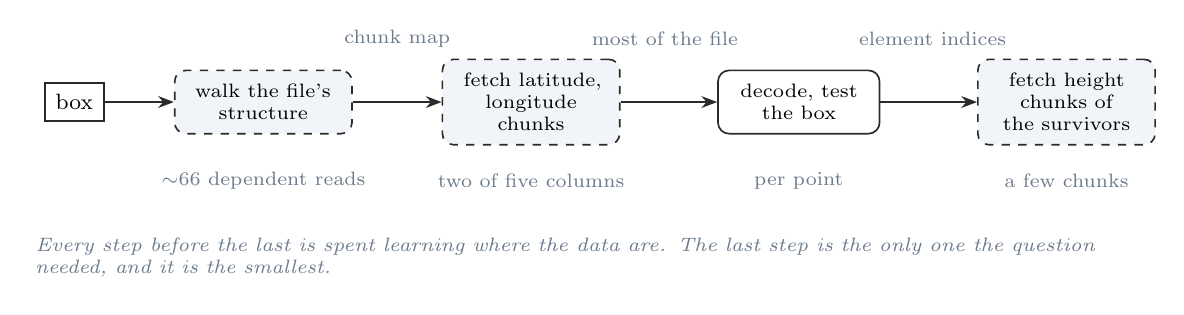
\begin{tikzpicture}[x=1mm,y=1mm]
  \node[val] (q) at (0,14) {box};
  \node[eff, text width=19mm, font=\scriptsize] (walk) at (24,14) {walk the file's structure};
  \node[eff, text width=19mm, font=\scriptsize] (fetch) at (58,14) {fetch latitude, longitude chunks};
  \node[pure, text width=17mm, font=\scriptsize] (dec) at (92,14) {decode, test the box};
  \node[eff, text width=19mm, font=\scriptsize] (fetch2) at (126,14) {fetch height chunks of the survivors};
  \draw[flow] (q) -- (walk); \draw[flow] (walk) -- (fetch); \draw[flow] (fetch) -- (dec); \draw[flow] (dec) -- (fetch2);
  \node[lbl] at (41,22) {chunk map}; \node[lbl] at (75,22) {most of the file}; \node[lbl] at (109,22) {element indices};
  \node[lbl] at (24,4) {$\sim$66 dependent reads}; \node[lbl] at (58,4) {two of five columns}; \node[lbl] at (92,4) {per point}; \node[lbl] at (126,4) {a few chunks};
  \node[note, text width=136mm, anchor=north west] at (-6,-2) {Every step before the last is spent learning where
    the data are. The last step is the only one the question needed, and it is the smallest.};
\end{tikzpicture}}
\caption{Finding a box's points in one along-track granule without an index. Position is data, so locating the
data means reading it; the structure walk and the position fetch dominate, and both must be repeated for every
granule and every query.}
\label{fig:wherelat}
\end{figure}

\paragraph{(d) The data are sparse and irregular.} Across track, a site is sampled where tracks happened to cross
it: for one 530\,m cell the ICESat-2 record gives 855 populated cells where GLAS gives 112 over the same area, and
IceBridge gives flight lines on 32 days in one cell and nothing in the next. In time, GLAS is 19 campaigns, GEDI
paused for most of 2023, IceBridge flew in seasons. A coverage question (Q2) is therefore a real question, not a
lookup, and a system that answers it by searching the catalogue returns the footprint's answer, which (a) showed is
wrong by a third.

\paragraph{(e) Holes and fills.} Points that exist in the file may carry no information: cloud returns, fill values
($1.798\times10^{308}$, $3.4\times10^{38}$), saturated or degraded flags. On the deployed instance 4.1\,\% of
the ATL06 cells a query selected turned out to name a chunk whose every point is fill. A system must keep the fact
that it looked, or it will look again forever.

\paragraph{(f) The catalogue has its own pitfalls.} Cloud-hosted and on-premises copies of the same granule are both
listed, so an unfiltered search returns every file twice (2\,898 hits against 1\,449 for one area). A mistyped
version returns zero granules silently, indistinguishable from an empty region. Polygon edges are great circles, so
a 1.7$^\circ$ edge at 69$^\circ$N bows 230\,m and silently excluded three of 688 granules until edges were
densified to 0.25$^\circ$. A polygon of 725 vertices exceeds the request-URI limit. None of these is a defect to fix;
they are the shape of a catalogue built for granule-level discovery, and a system that depends on it at query time
inherits all of them.

\paragraph{(g) Time is never a predicate.} With the clock encoded five ways and the granule as the unit, a time
window can only be a granule-level filter on the catalogue's time range, which is the same over-claim as (a) in
another dimension. Inside a granule, a window finer than its extent eliminates nothing a spatial predicate has not
already eliminated: an ATL06 granule inside one res-5 cell is a few seconds long.

\begin{table}[tbp]
\footnotesize
\wide{\begin{tabular}{@{}llrrrrrrrr@{}}
\toprule
area & source & CMR hits & GB & like-for-like & in cells & false pos. & need (MB) & ratio & footprint$\times$ \\
\midrule
summit & ATL06 & 549 & 45.0 & 726 & 656 & 9.6\,\% & 647 & 70 & 8.1 \\
summit & ATL03 & 602 & 1\,197 & 666 & 664 & 0.3\,\% & 12\,754 & 94 & 9.8 \\
summit & GLAS & 120 & 0.45 & 156 & 137 & 14.7\,\% & 70 & 6.4 & orbit \\
summit & ICESSN & 195 & 0.03 & 271 & 251 & 7.4\,\% & 25 & 1.3 & 0.0 \\
egig\_west\_flank & ATL06 & 553 & 48.6 & 761 & 665 & 12.6\,\% & 655 & 74 & 8.1 \\
egig\_west\_flank & ATL03 & 560 & 1\,040 & 656 & 600 & 8.5\,\% & 12\,072 & 86 & 8.5 \\
egig\_west\_flank & GLAS & 139 & 0.52 & 139 & 127 & 8.6\,\% & 65 & 8.0 & orbit \\
k\_transect & ATL06 & 557 & 49.9 & 649 & 579 & 11.1\,\% & 626 & 80 & 7.2 \\
k\_transect & GLAS & 108 & 0.40 & 140 & 102 & 27.1\,\% & 49 & 8.2 & orbit \\
jakobshavn & ATL06 & 571 & 47.1 & 749 & 644 & 14.0\,\% & 752 & 63 & 7.2 \\
jakobshavn & ATL03 & 576 & 1\,410 & 637 & 608 & 4.6\,\% & 20\,081 & 70 & 8.2 \\
jakobshavn & ICESSN & 504 & 0.14 & 882 & 775 & 12.1\,\% & 102 & 1.3 & 0.0 \\
summit\_traverse & ATL06 & 109 & 9.0 & 220 & 150 & 31.8\,\% & 105 & 86 & 852 \\
summit\_traverse & ATL03 & 116 & 234 & 175 & 144 & 17.7\,\% & 493 & 475 & 1\,009 \\
summit\_traverse & GLAS & 15 & 0.06 & 31 & 21 & 32.3\,\% & 11 & 5.3 & orbit \\
\bottomrule
\end{tabular}}
\caption{Catalogue search against the sub-granule index, measured 2026-10-19 on the deployed instance
(\code{scripts/measure\_search\_modes.py}; full table in Appendix~\ref{app:numbers}). \emph{CMR hits} and \emph{GB}
are the catalogue's answer for the box and its total granule size; \emph{like-for-like} is the catalogue's answer
for the outline of the box's cells, the same ground the index answers for; \emph{in cells} is the index's count of
granules with a point in those cells; \emph{false pos.} is the share of like-for-like hits with no such point;
\emph{need} is the bytes the index would fetch; \emph{ratio} is GB moved per GB needed; \emph{footprint}$\times$ is
the median catalogued footprint area over the box area (``orbit'': GLAS records carry orbit parameters only, so no polygon exists to measure; IceBridge polygons are the thin swath, so their area is a fraction of the box's).}
\label{tab:searchmodes}
\end{table}

\section{Requirements from first principles}
\label{ch:requirements}

Each failure in Chapter~\ref{ch:failures} says what a better system must record or do. We state the requirements
once, numbered, and every mechanism in the rest of the report is introduced as the discharge of one of them
(Figure~\ref{fig:reqmap}).

\begin{description}\setlength{\itemsep}{3pt}
\item[\req{1} Search by where the points are, not where the track was.] Failure (a). The system must hold, for every
  granule, a record of where its points fall, at a granularity fine enough to reject a granule that only brushes an
  area and coarse enough to be stored for fifty thousand granules. Such a record can be made only by reading the
  positions, so it is made \emph{once}, at build time, never at query time.
\item[\req{2} Retrieve by the storage unit.] Failures (b) and (c). The smallest thing the archive can serve is a
  byte range, and the smallest useful byte range is a chunk. The record of \req{1} must therefore be keyed by chunk
  and carry the chunk's (offset, size) for every dataset the query will want, so that a query goes from area to
  byte ranges without opening a file. The chunk map is read once, with the positions.
\item[\req{3} A discrete, hierarchical, integer spatial key.] The record of \req{1} needs a key that a point maps
  to by arithmetic, that a query area maps to as a finite set, that is an integer (so files, tables and set
  operations stay cheap), that nests (so coverage can be stated compactly at one resolution and checked at another),
  and whose cells are of roughly equal area (so a resolution means the same thing everywhere). This is the
  definition of a discrete global grid system; Part~\ref{part:dggs} chooses one.
\item[\req{4} Completeness must be provable.] Failures (a), (e) and (f). Silence is indistinguishable from
  absence: an empty answer may mean no data, a granule not yet indexed, a search that returned zero by mistake, or a
  cell whose every point was fill. The system must record what ground each build covered, which granules it looked
  at, and which filter set each granule's record was made against, and a query must refuse an area the record does
  not provably cover.
\item[\req{5} A query's cost is bounded by the network.] Failures (b) and (c). Once the index exists, the only
  irreducible cost of a query is fetching the bytes it names. Everything else (planning, deciding which points
  belong to which cell, decoding, caching) must cost less than the fetch, which means that work proportional to
  the number of points must be native and vectorised, or avoided by recording its answer in the index.
\item[\req{6} Repeated nearby queries reuse decoded points.] Chapter~\ref{ch:queries}. Decoded points must be kept
  in a local store keyed by the same cells as the index, read before any fetch, and safe to write from several
  threads at once, so that the second query over a site costs only its arithmetic.
\item[\req{7} A collection is data.] Tables~\ref{tab:logical}--\ref{tab:collections}. Six sources differ in a
  dozen named ways and in nothing else. The pipeline must be written once, over a description of the collection,
  so that a seventh source is a description and not a re-implementation.
\end{description}

\begin{figure}[tbp]
\wide{%
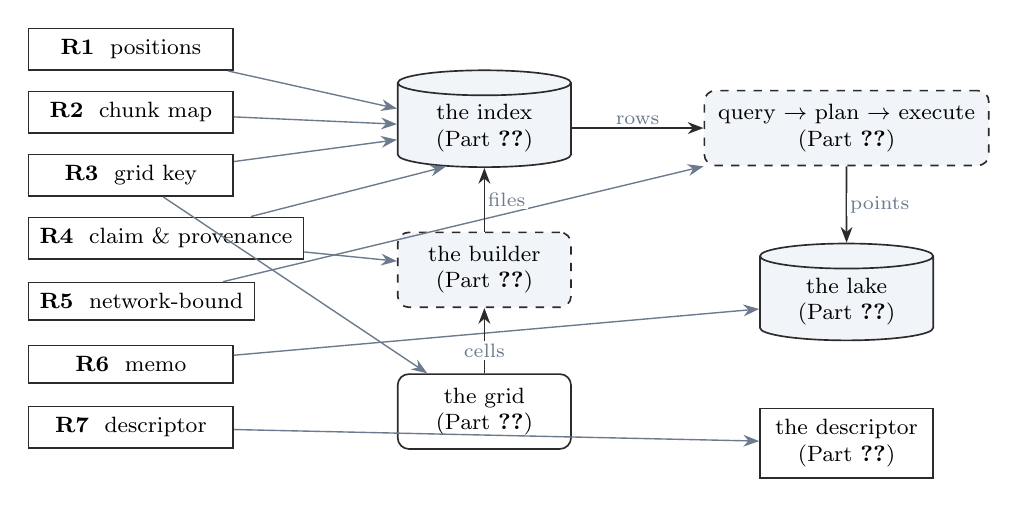
\begin{tikzpicture}[x=1mm,y=1mm]
  \foreach \y/\r/\t in {40/1/positions, 32/2/chunk map, 24/3/grid key, 16/4/claim \& provenance, 8/5/network-bound, 0/6/memo, -8/7/descriptor} {
    \node[val, anchor=west, minimum width=26mm] (r\r) at (0,\y) {\req{\r}\ \ \t};
  }
  \node[store, minimum width=22mm, minimum height=10mm] (idx) at (58,30) {the index\\(Part~\ref{part:index})};
  \node[eff, minimum width=22mm] (build) at (58,12) {the builder\\(Part~\ref{part:build})};
  \node[pure, minimum width=22mm] (grid) at (58,-6) {the grid\\(Part~\ref{part:dggs})};
  \node[eff, minimum width=22mm] (query) at (104,30) {query $\to$ plan $\to$ execute\\(Part~\ref{part:query})};
  \node[store, minimum width=22mm, minimum height=10mm] (lake) at (104,8) {the lake\\(Part~\ref{part:lake})};
  \node[val, minimum width=22mm] (desc) at (104,-10) {the descriptor\\(Part~\ref{part:framework})};
  \draw[flowsoft] (r1) -- (idx); \draw[flowsoft] (r2) -- (idx); \draw[flowsoft] (r3) -- (grid); \draw[flowsoft] (r3) -- (idx);
  \draw[flowsoft] (r4) -- (build); \draw[flowsoft] (r4) -- (idx.south west);
  \draw[flowsoft] (r5) -- (query.south west); \draw[flowsoft] (r6) -- (lake); \draw[flowsoft] (r7) -- (desc);
  \draw[flow] (idx) -- node[lblw, above] {rows} (query); \draw[flow] (build) -- node[lblw, right] {files} (idx);
  \draw[flow] (query) -- node[lblw, right] {points} (lake); \draw[flow] (grid) -- node[lblw, below] {cells} (build);
\end{tikzpicture}}
\caption{The requirements and the parts of the report that discharge them. The index is the centre: the grid keys
it, the builder writes it, the query reads it, the lake memoises what the query decoded, and the descriptor is the
one value that tells all of them which collection they are working on.}
\label{fig:reqmap}
\end{figure}

%=====================================================================================================================
\clearpage
\part{Discrete global grids}
\label{part:dggs}
%=====================================================================================================================

\section{What a discrete global grid system is}
\label{ch:dggs}

\req{3} asks for a spatial key with five properties: a point maps to it by arithmetic, an area maps to a finite set
of it, it is an integer, it nests across resolutions, and its cells have roughly equal area. A \emph{discrete
global grid system} (DGGS) is a family of partitions of the Earth's surface into cells, one partition per
resolution, with a scheme that assigns every cell an identifier and relates cells across
resolutions~\citep{sahr2003,ogc2021dggs}. The construction is always the same in outline (Figure~\ref{fig:dggs}):
choose a polyhedron that approximates the sphere, project its faces onto the surface, tile each face with a
regular pattern, and refine the pattern by a fixed \emph{aperture} (the number of children per parent) to make the
next resolution. The variations that matter to us are the polyhedron, the cell shape, the aperture, whether the
refinement is exact (every child lies inside its parent) and whether the identifier is an integer that encodes the
hierarchy.

\begin{figure}[tbp]
\wide{%
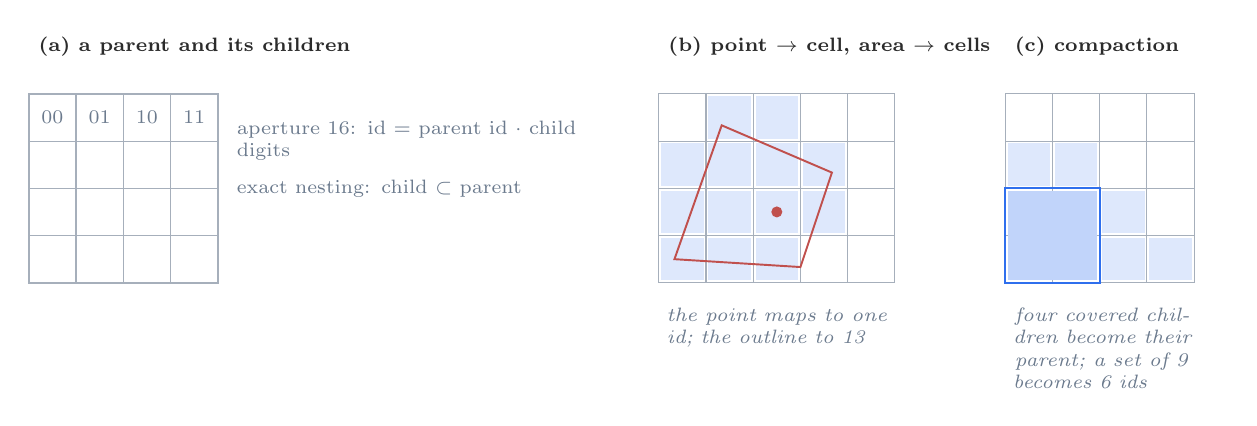
\begin{tikzpicture}[x=1mm,y=1mm]
  \node[hdr] at (0,30) {(a) a parent and its children};
  \draw[grid, line width=0.8pt] (0,0) rectangle (24,24);
  \foreach \x in {6,12,18} { \draw[grid] (\x,0) -- (\x,24); \draw[grid] (0,\x) -- (24,\x); }
  \node[lbl] at (3,21) {00}; \node[lbl] at (9,21) {01}; \node[lbl] at (15,21) {10}; \node[lbl] at (21,21) {11};
  \node[lbl, anchor=west, text width=46mm, align=left] at (26,18) {aperture 16: id $=$ parent id $\cdot$ child digits};
  \node[lbl, anchor=west, text width=46mm, align=left] at (26,12) {exact nesting: child $\subset$ parent};
  \node[hdr] at (80,30) {(b) point $\to$ cell, area $\to$ cells};
  \foreach \x in {80,86,...,104} { \foreach \y in {0,6,...,18} { \draw[grid] (\x,\y) rectangle (\x+6,\y+6); } }
  \foreach \x/\y in {80/0, 86/0, 92/0, 80/6, 86/6, 92/6, 98/6, 80/12, 86/12, 92/12, 98/12, 86/18, 92/18} { \fill[idxblue!16] (\x+0.3,\y+0.3) rectangle (\x+5.7,\y+5.7); }
  \fill[nasared] (95,9) circle (0.7);
  \draw[box] (82,3) -- (98,2) -- (102,14) -- (88,20) -- cycle;
  \node[note, text width=28mm, anchor=north west] at (80,-2) {the point maps to one id; the outline to 13};
  \node[hdr] at (124,30) {(c) compaction};
  \foreach \x in {124,130,...,142} { \foreach \y in {0,6,...,18} { \draw[grid] (\x,\y) rectangle (\x+6,\y+6); } }
  \fill[idxblue!30] (124.3,0.3) rectangle (135.7,11.7); \draw[draw=idxblue, line width=0.8pt] (124,0) rectangle (136,12);
  \foreach \x/\y in {136/0, 142/0, 136/6, 124/12, 130/12} { \fill[idxblue!16] (\x+0.3,\y+0.3) rectangle (\x+5.7,\y+5.7); }
  \node[note, text width=26mm, anchor=north west] at (124,-2) {four covered children become their parent; a set
    of 9 becomes 6 ids};
\end{tikzpicture}}
\caption{The three operations the index needs from a grid, shown on a square aperture-16 grid: the hierarchy
encoded in the identifier, point and area assignment, and compaction of a set up the hierarchy. Each real system
below realises them differently.}
\label{fig:dggs}
\end{figure}

What the index asks of these operations is specific, and worth stating as the tests a candidate grid must pass:

\begin{itemize}
\item \textbf{Point assignment} runs once per point at build time, for $10^{9}$ photons and $10^{8}$ segments. It
  must exist as a vectorised native kernel callable from Python over arrays; a scalar call per point is two orders of
  magnitude too slow.
\item \textbf{Area to cells} (``polyfill'') runs once per query and per build; it may be slow and must be exact
  in the sense of covering every cell the area overlaps, with a mode that excludes cells that merely share an edge.
\item \textbf{Identifiers} are stored once per index row and once per lake file name, and compared in set
  operations by the million. They must be 64-bit integers, or packable to them.
\item \textbf{Hierarchy} is used to compact a coverage claim and to test membership by walking ancestors. The
  identifier must yield the parent by arithmetic. Exact nesting of \emph{area} is a convenience the design must not
  rely on (Chapter~\ref{ch:gridhere}).
\item \textbf{Equal area} makes a resolution a statement about ground: ``resolution 5'' must mean about the same
  footprint at 60$^\circ$N and at 80$^\circ$N, or the chunk-to-cell ratio the index is tuned for drifts with
  latitude.
\item \textbf{Convex cells} along a straight track make the run of a cell's points inside a chunk contiguous
  (Chapter~\ref{ch:row}); a grid with concave cells forfeits that shortcut.
\end{itemize}

\section{Four systems}
\label{ch:foursystems}

\paragraph{H3.} Uber's H3 projects an icosahedron onto the sphere and tiles each face with hexagons; the twelve
icosahedron vertices carry pentagons~\citep{h3docs}. Resolution 0 has 122 base cells; each finer resolution has
aperture 7, so a cell has one seventh the area of its parent and the finest resolution, 15, is under a square metre.
Identifiers are 64-bit integers that encode the base cell and the sequence of child digits, so parent and children
are bit operations. Because an aperture-7 hexagon tiling cannot be made of hexagons that tile their parent exactly,
children are rotated by about 19.1$^\circ$ and straddle the parent's boundary: the hierarchy is exact in the
identifier and approximate in area. Cells are convex, neighbours are uniform (six, except at pentagons), and area
varies by about a factor of two across the globe at a given resolution. Vectorised kernels exist in Python through
h3ronpy. H3 is what the system uses today (Figure~\ref{fig:h3}).

\paragraph{S2.} Google's S2 projects a cube onto the sphere and tiles each face with a quadtree~\citep{s2docs}. A
cell at level $k$ is identified by a 3-bit face and $k$ two-bit child digits packed into a 64-bit integer whose
lowest set bit marks the level; the identifiers order cells along a Hilbert curve on each face, so consecutive
identifiers are spatially close, and a parent's identifier is the midpoint of its children's range. Nesting is
exact: a child lies inside its parent. Cells are quadrilaterals whose area varies by about a factor of two across
a face because the gnomonic projection stretches the edges. Polyfill is a covering by a bounded number of cells of
mixed level. Python bindings exist; a vectorised point kernel over arrays does not come with them
(Figure~\ref{fig:s2}).

\paragraph{HEALPix.} The Hierarchical Equal Area isoLatitude Pixelisation divides the sphere into twelve base
pixels of equal area, each refined by aperture 4 into pixels that remain exactly equal in area and whose centres lie
on rings of constant latitude~\citep{gorski2005}. The equal-area and iso-latitude properties exist for spherical
harmonic analysis of all-sky maps, which is its home. Nesting is exact and the ``nested'' numbering is hierarchical;
identifiers are integers (64 bits suffice to resolution 29). Pixels are curvilinear quadrilaterals, not convex in
the projected sense near the base-pixel corners. Vectorised kernels exist (healpy); polygon-to-pixel queries exist
but are coarse (Figure~\ref{fig:healpix}).

\paragraph{rHEALPix.} Gibb's rHEALPix rearranges the HEALPix projection so that the whole sphere maps onto a plane
of square cells with exact aperture-9 (or 4) nesting and exact equal area, and extends it to an ellipsoid of
revolution~\citep{gibb2016}. Cells are squares in the projection and quadrilaterals on the ground, with the polar
caps' squares distorted into triangles on the sphere. Identifiers are strings (a base cell letter and child
digits); they can be packed into integers but no standard library does so. It is an OGC-conformant DGGS and its
reference implementation is pure Python without a vectorised kernel (Figure~\ref{fig:rhealpix}).

\paragraph{The non-equal-area baseline.} Geohash and the web-map quadkey partition the latitude--longitude
rectangle, not the sphere, so a cell at 80$^\circ$N is a sixth the ground area of a cell at the equator. They are
cheap, hierarchical by string prefix, and everywhere. They fail the equal-area test badly enough for polar work
that we do not consider them further.

\begin{figure}[tbp]
\wide{%
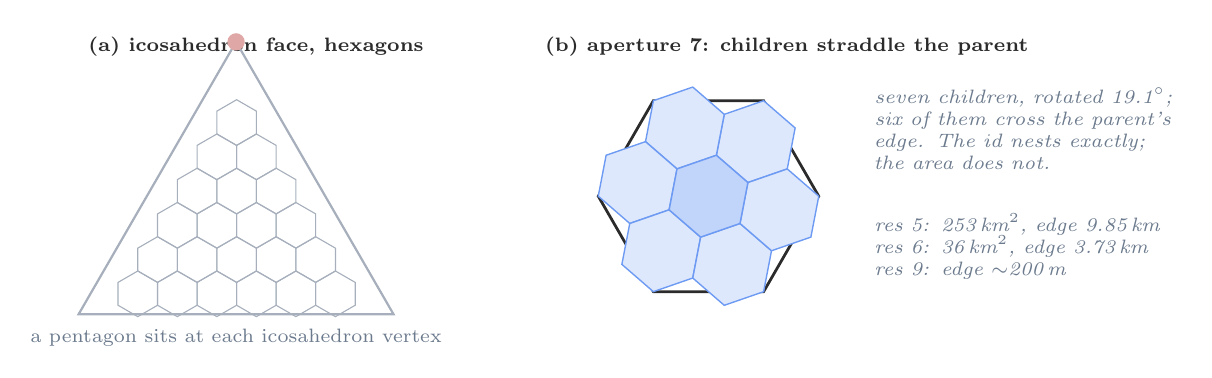
\begin{tikzpicture}[x=1mm,y=1mm]
  \node[hdr] at (0,34) {(a) icosahedron face, hexagons};
  \draw[grid, line width=0.8pt] (0,0) -- (40,0) -- (20,34.6) -- cycle;
  \foreach \i in {0,...,8} { \foreach \j in {0,...,7} {
    \pgfmathsetmacro{\cx}{2.5 + \i*5.02 + mod(\j,2)*2.51} \pgfmathsetmacro{\cy}{2.6 + \j*4.35}
    \pgfmathparse{(abs(\cx-20) < 20 - \cy/1.732 - 2.4) ? 1 : 0}
    \ifnum\pgfmathresult=1 \draw[grid] \hexp{\cx}{\cy}{2.9}{30}; \fi } }
  \fill[nasared!50] (20,34.6) circle (1.1); \node[lbl, anchor=north] at (20,-1.5) {a pentagon sits at each icosahedron vertex};
  \node[hdr] at (58,34) {(b) aperture 7: children straddle the parent};
  \draw[draw=ink, line width=1pt] \hexp{80}{15}{14}{0};
  \foreach \m in {0,...,5} {
    \pgfmathsetmacro{\px}{80 + 9.17*cos(49.1+60*\m)} \pgfmathsetmacro{\py}{15 + 9.17*sin(49.1+60*\m)}
    \fill[idxblue!16] \hexp{\px}{\py}{5.29}{19.1}; \draw[draw=idxblue!70, line width=0.5pt] \hexp{\px}{\py}{5.29}{19.1}; }
  \fill[idxblue!30] \hexp{80}{15}{5.29}{19.1}; \draw[draw=idxblue!70, line width=0.5pt] \hexp{80}{15}{5.29}{19.1};
  \node[note, text width=38mm, anchor=north west] at (100,30) {seven children, rotated 19.1$^\circ$; six of them
    cross the parent's edge. The id nests exactly; the area does not.};
  \node[note, text width=38mm, anchor=north west] at (100,14) {res 5: 253\,km$^2$, edge 9.85\,km\\res 6:
    36\,km$^2$, edge 3.73\,km\\res 9: edge $\sim$200\,m};
\end{tikzpicture}}
\caption{H3: hexagons on an icosahedron with aperture-7 refinement. Convex cells and uniform neighbours, 64-bit
identifiers with the hierarchy in the bits, and a refinement that is exact in identifiers but not in area.}
\label{fig:h3}
\end{figure}

\begin{figure}[tbp]
\wide{%
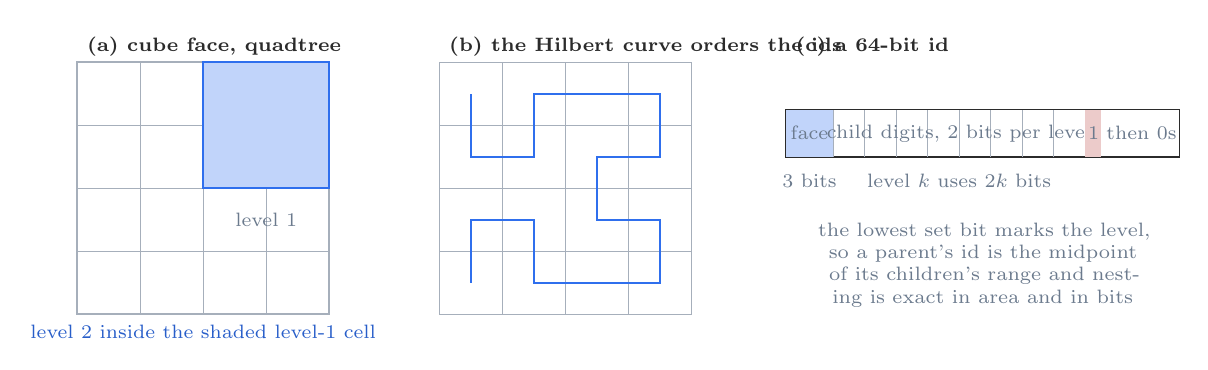
\begin{tikzpicture}[x=1mm,y=1mm]
  \node[hdr] at (0,34) {(a) cube face, quadtree};
  \draw[grid, line width=0.8pt] (0,0) rectangle (32,32);
  \foreach \x in {8,16,24} { \draw[grid] (\x,0) -- (\x,32); \draw[grid] (0,\x) -- (32,\x); }
  \foreach \x in {16,20,24,28} { \foreach \y in {16,20,24,28} { \draw[grid] (\x,\y) rectangle (\x+4,\y+4); } }
  \fill[idxblue!30] (16,16) rectangle (32,32); \draw[draw=idxblue, line width=0.8pt] (16,16) rectangle (32,32);
  \node[lbl] at (24,12) {level 1}; \node[lbl, text=idxblue!85!black, anchor=north] at (16,-1) {level 2 inside the shaded level-1 cell};
  \node[hdr] at (46,34) {(b) the Hilbert curve orders the ids};
  \foreach \x in {46,54,62,70} { \foreach \y in {0,8,16,24} { \draw[grid] (\x,\y) rectangle (\x+8,\y+8); } }
  \draw[track] (50,4) -- (50,12) -- (58,12) -- (58,4) -- (66,4) -- (74,4) -- (74,12) -- (66,12) -- (66,20) -- (74,20) -- (74,28) -- (66,28) -- (58,28) -- (58,20) -- (50,20) -- (50,28);
  \node[hdr] at (90,34) {(c) a 64-bit id};
  \draw[draw=ink, line width=0.5pt] (90,20) rectangle (140,26);
  \fill[idxblue!30] (90,20) rectangle (96,26); \node[lbl] at (93,23) {face}; \node[lbl] at (93,17) {3 bits};
  \foreach \x in {96,100,...,124} { \draw[grid] (\x,20) -- (\x,26); }
  \node[lbl] at (112,23) {child digits, 2 bits per level}; \node[lbl] at (112,17) {level $k$ uses $2k$ bits};
  \fill[nasared!30] (128,20) rectangle (130,26); \node[lbl] at (134,23) {1 then 0s};
  \node[lbl, text width=48mm, anchor=north] at (115,12) {the lowest set bit marks the level, so a parent's id is the midpoint of
    its children's range and nesting is exact in area and in bits};
\end{tikzpicture}}
\caption{S2: a quadtree on each face of a cube, identifiers along a Hilbert curve. Exact nesting and spatial
locality of identifiers; cells are quadrilaterals whose area varies across a face.}
\label{fig:s2}
\end{figure}

\begin{figure}[tbp]
\wide{%
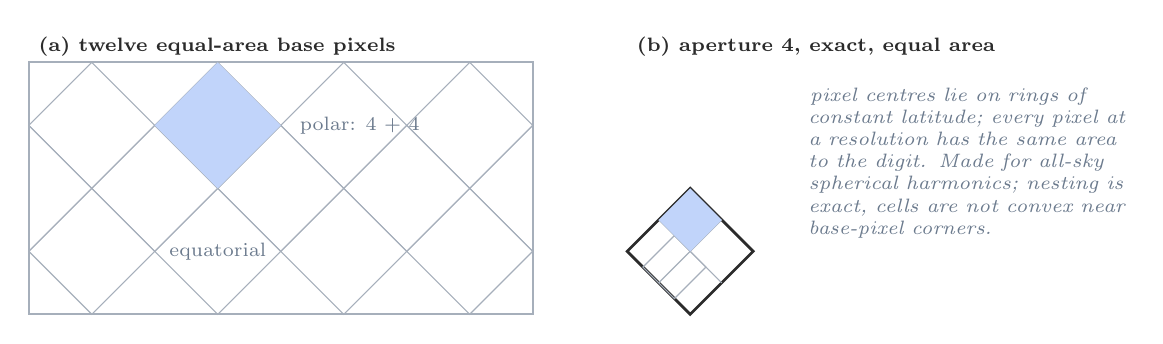
\begin{tikzpicture}[x=1mm,y=1mm]
  \node[hdr] at (0,34) {(a) twelve equal-area base pixels};
  \draw[grid, line width=0.8pt] (0,0) rectangle (64,32);
  % HEALPix projection: 4 polar diamonds top, 4 equatorial, 4 polar bottom (schematic)
  \foreach \k in {0,...,3} { \draw[grid] (8+16*\k,32) -- (16*\k,24) -- (8+16*\k,16) -- (16+16*\k,24) -- cycle; }
  \foreach \k in {0,...,3} { \draw[grid] (8+16*\k,0) -- (16*\k,8) -- (8+16*\k,16) -- (16+16*\k,8) -- cycle; }
  \foreach \k in {0,...,3} { \draw[grid] (16*\k,8) -- (8+16*\k,16) -- (16*\k,24) ; \draw[grid] (16+16*\k,8) -- (8+16*\k,16) -- (16+16*\k,24); }
  \fill[idxblue!30] (24,32) -- (16,24) -- (24,16) -- (32,24) -- cycle;
  \node[lbl] at (24,8) {equatorial}; \node[lbl, anchor=west] at (34,24) {polar: 4 + 4};
  \node[hdr] at (76,34) {(b) aperture 4, exact, equal area};
  \draw[draw=ink, line width=1pt] (84,0) -- (76,8) -- (84,16) -- (92,8) -- cycle;
  \draw[grid] (80,4) -- (88,12); \draw[grid] (80,12) -- (88,4);
  \draw[grid] (82,2) -- (78,6) -- (82,10) -- (86,6) -- cycle;
  \fill[idxblue!30] (84,8) -- (80,12) -- (84,16) -- (88,12) -- cycle;
  \node[note, text width=40mm, anchor=north west] at (98,30) {pixel centres lie on rings of constant latitude;
    every pixel at a resolution has the same area to the digit. Made for all-sky spherical harmonics; nesting is
    exact, cells are not convex near base-pixel corners.};
\end{tikzpicture}}
\caption{HEALPix: twelve base pixels refined by aperture 4 into exactly equal-area pixels on iso-latitude rings.
Exact nesting, integer nested identifiers, vectorised kernels; cell shape is a curvilinear quadrilateral.}
\label{fig:healpix}
\end{figure}

\begin{figure}[tbp]
\wide{%
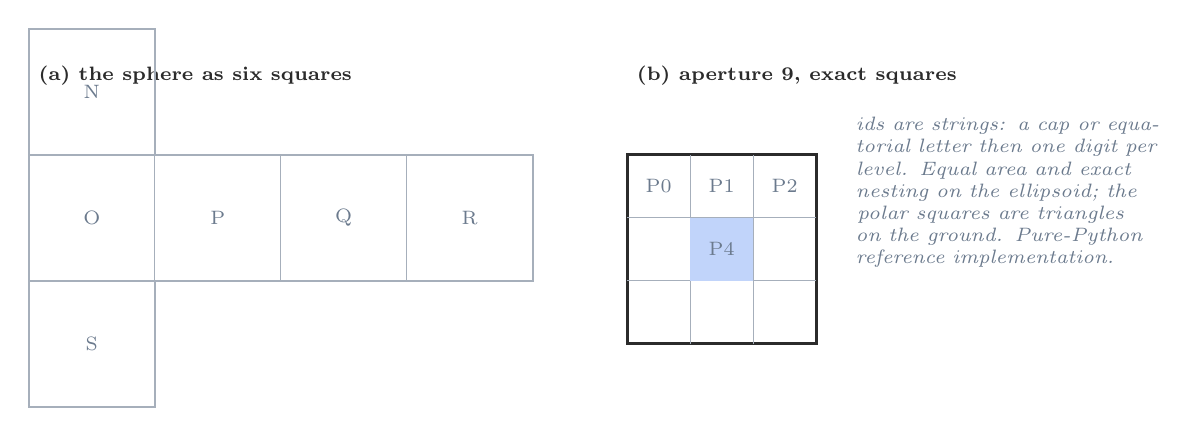
\begin{tikzpicture}[x=1mm,y=1mm]
  \node[hdr] at (0,34) {(a) the sphere as six squares};
  \draw[grid, line width=0.8pt] (0,8) rectangle (64,24);
  \foreach \x in {16,32,48} { \draw[grid] (\x,8) -- (\x,24); }
  \draw[grid, line width=0.8pt] (0,24) rectangle (16,40); \draw[grid, line width=0.8pt] (0,-8) rectangle (16,8);
  \node[lbl] at (8,32) {N}; \node[lbl] at (8,0) {S}; \foreach \x/\l in {8/O, 24/P, 40/Q, 56/R} { \node[lbl] at (\x,16) {\l}; }
  \node[hdr] at (76,34) {(b) aperture 9, exact squares};
  \draw[draw=ink, line width=1pt] (76,0) rectangle (100,24);
  \foreach \x in {84,92} { \draw[grid] (\x,0) -- (\x,24); \draw[grid] (76,\x-76) -- (100,\x-76); }
  \fill[idxblue!30] (84,8) rectangle (92,16); \node[lbl] at (88,12) {P4};
  \node[lbl] at (80,20) {P0}; \node[lbl] at (88,20) {P1}; \node[lbl] at (96,20) {P2};
  \node[note, text width=38mm, anchor=north west] at (104,30) {ids are strings: a cap or equatorial letter then
    one digit per level. Equal area and exact nesting on the ellipsoid; the polar squares are triangles on the
    ground. Pure-Python reference implementation.};
\end{tikzpicture}}
\caption{rHEALPix: HEALPix rearranged onto a plane of squares with aperture-9 refinement. Exact equal area and
exact nesting; string identifiers; no vectorised kernel in the reference library.}
\label{fig:rhealpix}
\end{figure}

\begin{table}[tbp]
\scriptsize
\wide{\begin{tabular}{@{}p{30mm}p{30mm}p{30mm}p{30mm}p{28mm}@{}}
\toprule
property (test) & H3 & S2 & HEALPix & rHEALPix \\
\midrule
polyhedron, cell shape & icosahedron, hexagon (12 pentagons) & cube, quadrilateral & 12 base pixels, curvilinear quad & 6 squares (plane), quad / triangle \\
aperture & 7 & 4 & 4 & 9 (or 4) \\
identifier & 64-bit int, hierarchy in bits & 64-bit int, Hilbert order & int, nested or ring & string; packable \\
nesting in area & approximate (19.1$^\circ$ twist) & exact & exact & exact \\
equal area & $\sim$2$\times$ variation & $\sim$2$\times$ per face & exact & exact \\
convex cells & yes & yes & not at corners & yes (projected) \\
neighbours & 6 (5 at pentagons) & 4 edge + corners, mixed level & 8, irregular at corners & 8 \\
polyfill with overlap mode & yes & covering, mixed level & coarse & yes \\
compaction & yes & yes (cell union) & by numbering & yes \\
vectorised point kernel (Python) & h3ronpy & no & healpy & no \\
\bottomrule
\end{tabular}}
\caption{The four systems against the tests of Chapter~\ref{ch:dggs}. No system passes all of them; the deciding
rows for a build over $10^{9}$ points are the kernel and the identifier, and only H3 and HEALPix pass both.}
\label{tab:grids}
\end{table}

\section{The grid in this system}
\label{ch:gridhere}\label{ch:cells}

The system uses H3. The decision rests on three rows of Table~\ref{tab:grids}: integer identifiers with the
hierarchy in the bits (set operations, parent walks and compaction are arithmetic), a vectorised assignment kernel
(the build's per-point cost), and convex cells (the contiguous-run shortcut of Chapter~\ref{ch:row}). HEALPix passes
the first two and loses on the third and on tooling for polygon queries; S2 and rHEALPix lose on the kernel. What
H3 gives up, exact nesting of area, the design is written not to need. Chapter~\ref{ch:grid} returns to the
question as a parameter: the properties relied on are few enough to be named, and a grid that supplies them can
replace H3 behind one value.

\paragraph{Resolutions.} A resolution is chosen per collection so that a cell is roughly the ground footprint of
one chunk: resolution 5 (253\,km$^2$, edge 9.85\,km) for ATL06, GLAS and IceBridge, whose chunks or arcs are
hundreds of kilometres long; resolution 6 (36\,km$^2$, edge 3.73\,km) for ATL03, whose 100\,000-photon chunks are
about 70\,km. Finer buys nothing on a scene-sized query and multiplies the index: the 2\,016\,842 resolution-5
cells of the globe become 14\,117\,882 at resolution 6. Analysis uses resolution 8 (about 530\,m) for per-cell time
series, and coverage claims are stated at resolution 9 (edge about 200\,m) so that a claim follows a drawn shape
closely; a claim is held under 60\,000 cells by backing off one resolution at a time.

\paragraph{Three roles.} A cell plays three roles, at two resolutions (Figure~\ref{fig:cells}). \emph{Addressing}:
every index row carries the cell of its points at the collection's addressing resolution, and a query turns its
area into the set of addressing cells it overlaps and asks the index for rows with those cells.
\emph{Partitioning}: the lake of decoded points is partitioned by the same cell, so a query reads exactly the cells
it asked for and eviction has a unit. \emph{Claiming}: a build records the ground it covered as a set of finer
cells, compacted up the hierarchy; a later query checks that every fine cell of its area has an ancestor in the
claim, and a later build over a larger area builds only the fine cells not yet claimed.

\begin{figure}[tbp]
\wide{%
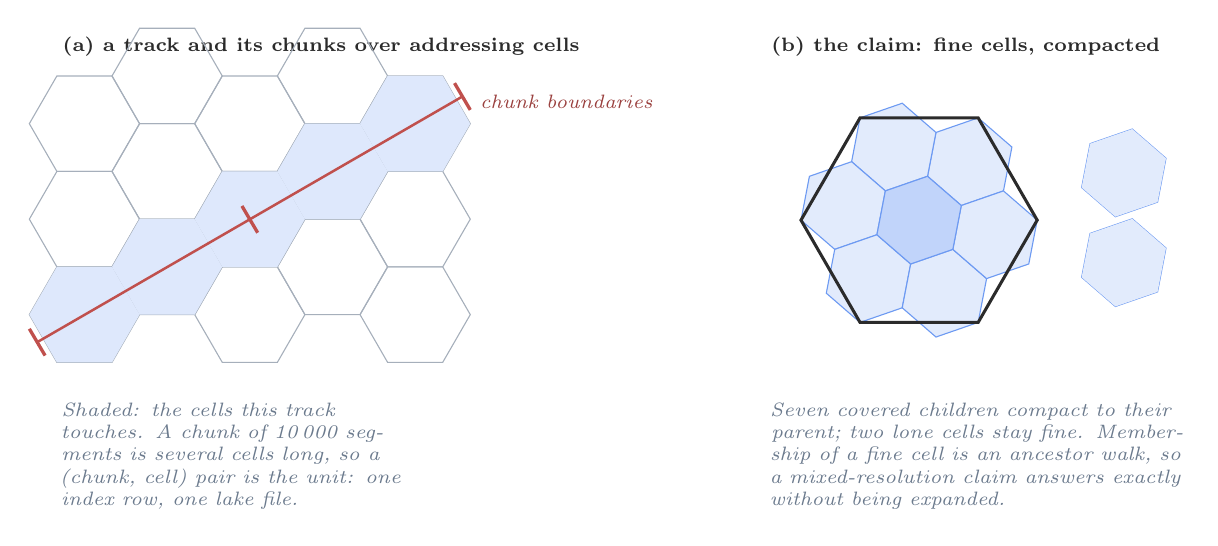
\begin{tikzpicture}[x=1mm,y=1mm,font=\footnotesize]
  \begin{scope}
    \node[hdr] at (-4,34) {(a) a track and its chunks over addressing cells};
    \foreach \i in {0,2,4} { \foreach \j in {0,1,2} {
      \draw[draw=soft!60, line width=0.4pt] \hexp{10.5*\i}{12.124*\j}{7}{0}; } }
    \foreach \i in {1,3} { \foreach \j in {0,1,2} {
      \draw[draw=soft!60, line width=0.4pt] \hexp{10.5*\i}{12.124*\j+6.062}{7}{0}; } }
    \fill[idxblue!16] \hexp{10.5}{6.062}{7}{0}; \fill[idxblue!16] \hexp{21}{12.124}{7}{0}; \fill[idxblue!16] \hexp{31.5}{18.186}{7}{0};
    \fill[idxblue!16] \hexp{0}{0}{7}{0}; \fill[idxblue!16] \hexp{42}{24.248}{7}{0};
    \draw[draw=nasared, line width=0.9pt] (-6,-3.5) -- (48,27.7);
    \foreach \s in {0,0.5,1} { \draw[draw=nasared, line width=1.2pt] ({-6+54*\s-1},{-3.5+31.2*\s+1.7}) -- ({-6+54*\s+1},{-3.5+31.2*\s-1.7}); }
    \node[note, anchor=west, text=nasared!80!black] at (49,27) {chunk boundaries};
    \node[note, text width=44mm, anchor=north west] at (-4,-10) {Shaded: the cells this track touches. A chunk of
      10\,000 segments is several cells long, so a (chunk, cell) pair is the unit: one index row, one lake file.};
  \end{scope}
  \begin{scope}[shift={(96,0)}]
    \node[hdr] at (-10,34) {(b) the claim: fine cells, compacted};
    \foreach \m in {0,...,5} {
      \fill[idxblue!14] \hexp{9.821*cos(49.106+60*\m)+10}{9.821*sin(49.106+60*\m)+12}{5.669}{19.106};
      \draw[draw=idxblue!70, line width=0.4pt] \hexp{9.821*cos(49.106+60*\m)+10}{9.821*sin(49.106+60*\m)+12}{5.669}{19.106}; }
    \fill[idxblue!30] \hexp{10}{12}{5.669}{19.106}; \draw[draw=idxblue!70, line width=0.4pt] \hexp{10}{12}{5.669}{19.106};
    \draw[draw=ink, line width=1.1pt] \hexp{10}{12}{15}{0};
    \draw[draw=idxblue!70, line width=0.4pt] \hexp{36}{18}{5.669}{19.106}; \fill[idxblue!14] \hexp{36}{18}{5.669}{19.106};
    \draw[draw=idxblue!70, line width=0.4pt] \hexp{36}{6.6}{5.669}{19.106}; \fill[idxblue!14] \hexp{36}{6.6}{5.669}{19.106};
    \node[note, text width=52mm, anchor=north west] at (-10,-10) {Seven covered children compact to their parent;
      two lone cells stay fine. Membership of a fine cell is an ancestor walk, so a mixed-resolution claim answers
      exactly without being expanded.};
  \end{scope}
\end{tikzpicture}}
\caption{Cells in two of their three roles. Left, addressing: index rows and lake files are keyed by (chunk, cell). Right,
claiming: the ground a build covered, stored compactly, consulted by every query and every enlarging build.}
\label{fig:cells}
\end{figure}

Two consequences shape everything downstream. First, a cell is coarse relative to a box, so the index over-selects
by design and the query re-applies the exact box predicate to decoded points; the index is for finding bytes, never
for answering the box. Second, the per-point assignment of a cell is the one operation the system performs
\emph{per point} on both sides, build and query, and it is the first thing to remove from the query side
(Chapter~\ref{ch:row}).\landed{\code{planner.cells\_for\_bbox}, \code{coverage\_cells}, \code{addressing\_cells},
\code{search\_polygon}; the claim in \code{index.write\_build\_manifest} and \code{unclaimed\_cells}; the hot kernel
is \code{planner.\_cells\_vectorized} over h3ronpy.}

\paragraph{Area to cells.} A rectangle or polygon becomes its set of overlapping cells with the library's
``overlap'' containment, after the shape is shrunk by $2\times10^{-6}$ degrees so that a cell which only shares an
edge with the shape is not included. The cells over-cover the shape by up to one cell edge (10\,km at resolution 5,
3.7\,km at 6), so every query re-applies the exact shape to the points it decodes; the index finds bytes, it never
answers the box. The cells also decide what the catalogue is asked at build time: their convex hull, densified to
0.25$^\circ$ edges so that great-circle bowing stays under five metres, is the search polygon, and it returns 688
granules where the exact outline would return 595.

\paragraph{Compaction and membership.} A claim of 3\,930 resolution-9 cells over a corridor compacts to 1\,188
identifiers by replacing every complete set of seven children with their parent, recursively. Whether a fine cell
is covered is then an ancestor walk, one parent operation per resolution step, with no expansion of the compacted
set. Because H3's children straddle their parent, a compacted claim is a statement about \emph{identifiers}, not
about ground: it means ``every one of these cells' descendants at the claim resolution was built'', which is exactly
what the query asks, and nothing about the parent hexagon's outline is assumed.

\clearpage
\part{The index}
\label{part:index}
%=====================================================================================================================

\section{The index as a relation}
\label{ch:row}

This chapter discharges \req{1} and \req{2}: a record, per granule, of where its points are, keyed by the storage
unit and carrying the byte ranges that unit occupies. Logically the index is one relation, (granule, group, chunk,
cell) $\to$ (byte range per dataset, chunk bounding box, run), and we derive it here; its physical form is the next
chapter. Everything in Parts~I--III can be assembled into the row the build writes. Take one granule, one group, one chunk $k$.
The build has the positions of the chunk's elements (read once, from the position datasets or the segment table),
assigns each its addressing cell, and so knows the set of cells the chunk touches. For each such cell it writes one
row. The row has four parts:

\begin{itemize}
\item \textbf{Identity}: granule name, both URLs (HTTPS and \code{s3://}), the archive revision, the group
  (beam) and whether it is a strong beam, orbit numbers, the chunk index and the element interval the chunk covers.
\item \textbf{The cell}, and the chunk's own bounding box in latitude and longitude. The box is a second, finer
  filter: a cell reaches kilometres outside a small query box, and the chunk's box prunes rows the cell let through.
\item \textbf{The run}: where, inside the chunk, this cell's elements sit. Below.
\item \textbf{Byte ranges}, one per dataset: offset, size, the filter pipeline, dtype, column count and the per-chunk
  filter mask. This is the chunk map of Figure~\ref{fig:chunkmap}, copied so the file need never be opened again.
\end{itemize}

Rows are few: a granule contributes about 18 rows for ATL06, 7 for ATL03, 25 for GLAS, 2 for ICESSN, because a
chunk is long and a cell is large. The same chunk appears under every cell it touches, with identical byte ranges;
the query deduplicates by (granule, group, chunk) before fetching.

\subsection{The run}

The build already paid for the one per-point operation: it assigned every positioned element its cell. Without the
run, the query would pay it again on every fetched chunk, because after decoding it has 10{,}000 segments or
100{,}000 photons and must know which of them belong to the cells it asked for. On the deployed machine that
re-assignment was 59 million lookups and 24 to 31 thread-seconds of an 8-cell query.

The run records what the build learned (Figure~\ref{fig:runs}). For a (chunk, cell) row:
\begin{align*}
[\code{run\_lo},\ \code{run\_hi}) &= \bigl[\min i,\ \max i + 1\bigr) \quad\text{over this cell's elements } i,\\
\code{run\_exact} &= \bigl(\#\{i \in [\code{lo},\code{hi}) \text{ positioned}\} = \#\{i \text{ in this cell}\}\bigr).
\end{align*}
Exactness is decidable at build time because the build has every element's cell. It says: no element of another
cell sits inside this interval. When every wanted cell's run is exact, the query labels the chunk's elements by
slicing, in constant time per cell, and never calls the grid. A straight-ish track meets a convex cell in one
contiguous stretch, so runs are exact unless cells interleave; on real ATL06 data 99.3\,\% of 9{,}422 runs over
twelve granules are exact, and in an 8-cell ingest all 2{,}948 chunks were labelled from runs.

\begin{figure}[tbp]
\wide{%
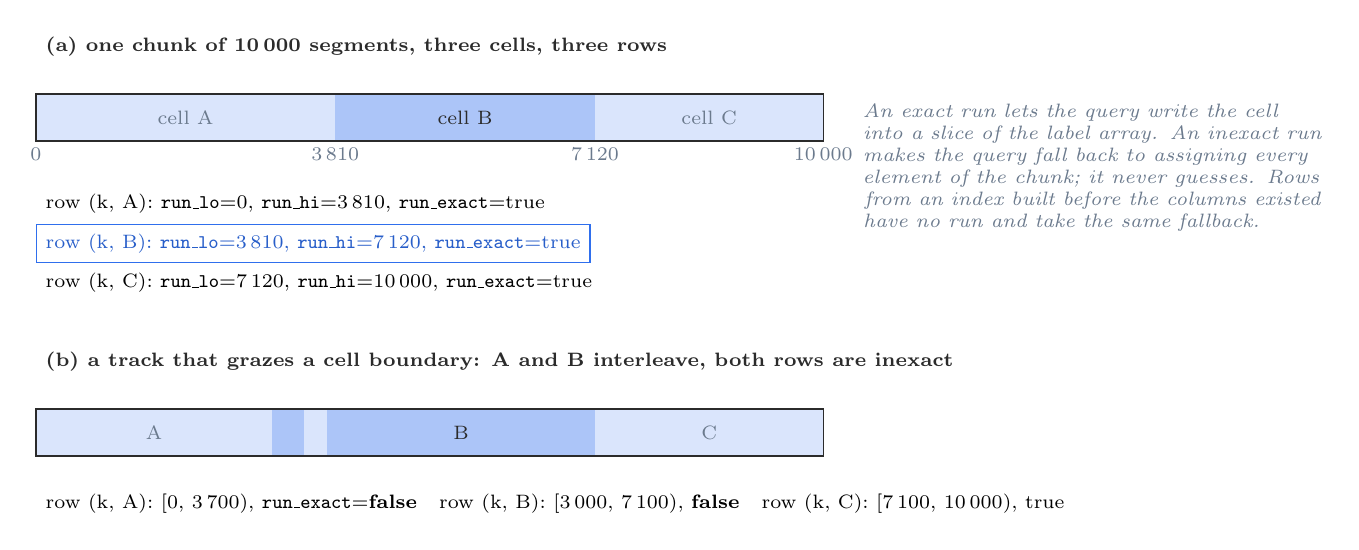
\begin{tikzpicture}[x=1mm,y=1mm]
  \node[hdr] at (0,30) {(a) one chunk of 10\,000 segments, three cells, three rows};
  \draw[draw=ink, line width=0.6pt] (0,18) rectangle (100,24);
  \fill[idxblue!18] (0,18) rectangle (38,24); \fill[idxblue!40] (38,18) rectangle (71,24); \fill[idxblue!18] (71,18) rectangle (100,24);
  \draw[draw=ink, line width=0.6pt] (0,18) rectangle (100,24);
  \node[lbl] at (19,21) {cell A}; \node[lbl, text=ink] at (54.5,21) {cell B}; \node[lbl] at (85.5,21) {cell C};
  \node[lbl, anchor=north] at (0,17.5) {0}; \node[lbl, anchor=north] at (38,17.5) {3\,810}; \node[lbl, anchor=north] at (71,17.5) {7\,120}; \node[lbl, anchor=north] at (100,17.5) {10\,000};
  \node[font=\scriptsize, anchor=west] at (0,10) {row (k, A): \code{run\_lo}=0, \code{run\_hi}=3\,810, \code{run\_exact}=true};
  \node[font=\scriptsize, anchor=west, acc] at (0,5) {row (k, B): \code{run\_lo}=3\,810, \code{run\_hi}=7\,120, \code{run\_exact}=true};
  \node[font=\scriptsize, anchor=west] at (0,0) {row (k, C): \code{run\_lo}=7\,120, \code{run\_hi}=10\,000, \code{run\_exact}=true};
  \node[hdr] at (0,-10) {(b) a track that grazes a cell boundary: A and B interleave, both rows are inexact};
  \draw[draw=ink, line width=0.6pt] (0,-22) rectangle (100,-16);
  \fill[idxblue!18] (0,-22) rectangle (30,-16); \fill[idxblue!40] (30,-22) rectangle (34,-16); \fill[idxblue!18] (34,-22) rectangle (37,-16);
  \fill[idxblue!40] (37,-22) rectangle (71,-16); \fill[idxblue!18] (71,-22) rectangle (100,-16);
  \draw[draw=ink, line width=0.6pt] (0,-22) rectangle (100,-16);
  \node[lbl] at (15,-19) {A}; \node[lbl, text=ink] at (54,-19) {B}; \node[lbl] at (85.5,-19) {C};
  \node[font=\scriptsize, anchor=west] at (0,-28) {row (k, A): [0, 3\,700), \code{run\_exact}=\textbf{false}\quad row (k, B): [3\,000, 7\,100), \textbf{false}\quad row (k, C): [7\,100, 10\,000), true};
  \node[note, text width=58mm, anchor=north west] at (104,24) {An exact run lets the query write the cell into a
    slice of the label array. An inexact run makes the query fall back to assigning every element of the chunk; it
    never guesses. Rows from an index built before the columns existed have no run and take the same fallback.};
\end{tikzpicture}}
\caption{Cell runs. Each row carries the element interval of its cell inside the chunk and whether that interval
is pure. The fast path is a slice; the slow path is the per-point assignment, kept alive by every inexact row.}
\label{fig:runs}
\end{figure}

The two pure kernels are short enough to show whole, because they \emph{are} the contract between build and
query:\landed{\code{index.cell\_runs}, \code{index.cells\_from\_runs}; the ATL06, GLAS and GEDI builders write
\code{run\_lo/run\_hi/run\_exact} (schema versions 3, 3, 2); their ingests slice. Counter
\code{chunks\_cells\_from\_runs} in the fetch stats.}

\begin{lstlisting}
def cell_runs(pos, cells) -> dict[int, tuple[int, int, bool]]:
    """{cell: (lo, hi, exact)} for one chunk; pos are within-chunk positions of its
    positioned points, cells their cells."""
    order = np.argsort(pos, kind="stable"); pos, cells = pos[order], cells[order]
    out = {}
    for cell in np.unique(cells):
        idx = np.flatnonzero(cells == cell)
        lo, hi = int(pos[idx[0]]), int(pos[idx[-1]]) + 1
        inside = np.searchsorted(pos, hi) - np.searchsorted(pos, lo)   # positioned points in [lo, hi)
        out[int(cell)] = (lo, hi, inside == idx.size)
    return out

def cells_from_runs(n, runs, wanted) -> np.ndarray | None:
    """Labels for a chunk's n points, or None when the fast path does not apply."""
    if not runs: return None
    out = np.zeros(n, "u8")
    for cell in wanted:
        r = runs.get(int(cell))
        if r is None or not r[2]: return None      # missing or inexact: fall back
        out[r[0]:r[1]] = int(cell)
    return out
\end{lstlisting}

\subsection{Photons: runs with edges}

ATL03 complicates the run in one way, because a photon's cell is known to the build only through its segment.
The build assigns a cell to each 20\,m segment from its reference photon and expresses the run in photon index
space: $[\code{run\_lo}, \code{run\_hi})$ is the union of the cell's segments' photon ranges inside the chunk. But
a segment straddling the cell boundary has photons on both sides, and the index must not claim for a cell photons
that belong to its neighbour. So the row records two more numbers, \code{edge\_lo\_end} and \code{edge\_hi\_start}:
where the run's first segment ends and where its last begins (Figure~\ref{fig:photonruns}). The query labels the
interior by slicing and assigns the grid cell individually only to the photons of the two edge segments, and to
photons outside every wanted run. The result is photon-exact, byte-identical to assigning all 100{,}000, at a few
hundred lookups.\landed{\code{index.photon\_cell\_runs}, \code{labels\_from\_photon\_runs}; ATL03 schema
version 6; the planner's \code{\_materialize} assigns only where \code{assign} is set and reports
\code{photons\_assigned}.}

\begin{figure}[tbp]
\wide{%
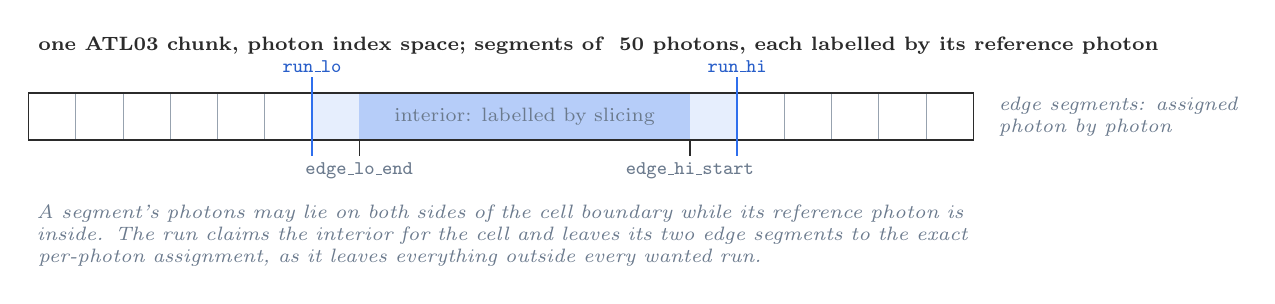
\begin{tikzpicture}[x=1mm,y=1mm]
  \node[hdr] at (0,22) {one ATL03 chunk, photon index space; segments of ~50 photons, each labelled by its reference photon};
  \draw[draw=ink, line width=0.6pt] (0,10) rectangle (120,16);
  \foreach \x in {0,6,...,114} \draw[draw=soft!70, line width=0.3pt] (\x,10) -- (\x,16);
  \fill[idxblue!35] (42,10) rectangle (84,16);
  \fill[idxblue!12] (36,10) rectangle (42,16); \fill[idxblue!12] (84,10) rectangle (90,16);
  \draw[draw=ink, line width=0.6pt] (0,10) rectangle (120,16);
  \draw[draw=idxblue, line width=0.9pt] (36,8) -- (36,18); \draw[draw=idxblue, line width=0.9pt] (90,8) -- (90,18);
  \node[lbl, text=idxblue!85!black, anchor=south] at (36,18.2) {\code{run\_lo}}; \node[lbl, text=idxblue!85!black, anchor=south] at (90,18.2) {\code{run\_hi}};
  \draw[draw=ink, line width=0.5pt] (42,8) -- (42,10); \draw[draw=ink, line width=0.5pt] (84,8) -- (84,10);
  \node[lbl, anchor=north] at (42,7.5) {\code{edge\_lo\_end}}; \node[lbl, anchor=north] at (84,7.5) {\code{edge\_hi\_start}};
  \node[lbl] at (63,13) {interior: labelled by slicing};
  \node[note, anchor=west] at (122,13) {edge segments: assigned\\photon by photon};
  \node[note, text width=118mm, anchor=north west] at (0,3) {A segment's photons may lie on both sides of the cell
    boundary while its reference photon is inside. The run claims the interior for the cell and leaves its two
    edge segments to the exact per-photon assignment, as it leaves everything outside every wanted run.};
\end{tikzpicture}}
\caption{Photon runs. The interior of a cell's run is labelled by slicing; the two edge segments and all photons
outside wanted runs are assigned individually, so the result equals assigning every photon.}
\label{fig:photonruns}
\end{figure}

\section{The index as files}
\label{ch:claim}

This chapter discharges \req{4}: the index must prove what it covers. Physically the relation of
Chapter~\ref{ch:row} is a set of Parquet files~\citep{parquetformat} plus three small side structures (Figure~\ref{fig:stores}), and the
proof lives in how they are named, stamped and folded.

The rows of one granule are one Parquet file, named after the granule, under the collection's index directory.
Writes are to a temporary name followed by a rename, so a reader never sees a torn file and an interrupted build
leaves no corpse for the next run to trip on. The file is the unit of resumption: a build lists the directory, and
a granule whose file exists with the current schema version is done.

That rule has a hole, and closing it is what the rest of this chapter is about. A build over a region asks for
rows only in the cells of that region: a granule's pole-to-pole track would otherwise fill the index with cells no
query ever asked for, each holding only the granules that happened to cross the region. So a granule's file is
\emph{relative to the cells the build asked for}, and a later build over a larger region cannot tell from the name
whether the file holds rows for the added ground.

\paragraph{Provenance.} Each file's footer therefore records the build's filter set: the compacted cell set the
build asked for, stored once as a content-addressed sidecar (\code{\_cellsets/<sha1>.json}) and referenced by its
hash.\side{The full compacted list was first stamped into every footer; at 49\,KB it was three quarters of an ATL06
index file and 3.3\,GB of a 7\,GB store. The sidecar took the store to 4.7\,GB.} A granule \emph{proves} a set of
cells if its recorded set contains them. An enlarging build computes the fine cells not yet claimed and rebuilds
exactly the granules that cannot prove them.

The invariant is easy to state and was broken twice: the footer must record the \emph{filter}, never the cells the
granule happened to touch. Two builders had shadowed the filter variable with the per-point cell array. For GLAS
the recorded set was touched\,$\cap$\,filter, which was never wrong but gave every granule its own sidecar (4{,}220
for 4{,}799 files) and rebuilt everything on every enlargement. For ATL03 it was the unfiltered touched set of the
last beam, so a file whose rows had been dropped could prove ground it did not hold, and an enlarging build silently
skipped it: the exact class of bug provenance exists to prevent.\landed{fixed 2026-10-17; the footer key is
\code{aicesat\_index\_cellset\_sha1}; \code{index.granule\_proves} answers False for unknown provenance;
\code{tests/test\_build\_provenance.py} pins both builders with a two-cell track and a one-cell filter.}

\paragraph{The claim.} When every granule of a build has landed, and only then, the build unions its fine cells
into the collection's claim (\code{\_build.json}): the compacted set of ground the index covers. Every query checks
its area against the claim before doing anything else; an unclaimed area is an error naming the build command, not
a slow success through whole-granule fallback. An empty catalogue search is recorded but claims nothing: silence from
the catalogue is not evidence of empty ground.

\paragraph{The manifest.} Coverage questions (which granules touch these cells, over which months) should not open
tens of thousands of footers. The build ends by folding the index into one small manifest of distinct (cell,
granule, month) rows (\code{\_coverage/manifest.parquet}), rebuilt whenever the directory's modification time says
a file landed. The query uses it to name the handful of files that touch its cells, so a plan reads a few files
rather than a glob of 48{,}838.\side{Before the manifest the ATL03 plan for a 0.3$^\circ$ box scanned every
footer: 36\,s. Through the manifest, 0.66\,s.}

\begin{figure}[tbp]
\wide{%
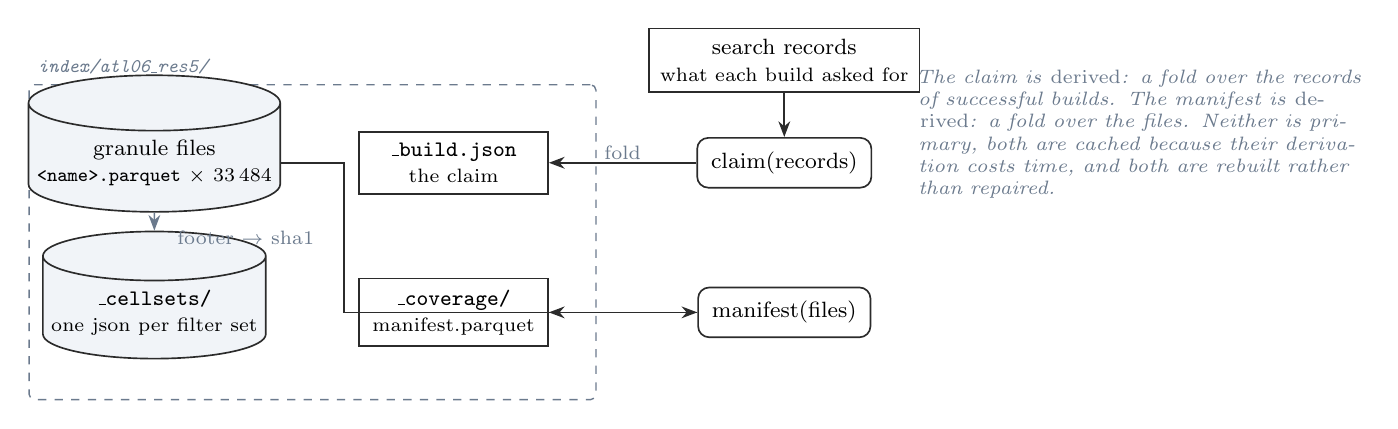
\begin{tikzpicture}[x=1mm,y=1mm]
  \node[proc, minimum width=72mm, minimum height=40mm, anchor=north west] (dir) at (0,43) {};
  \node[note, anchor=south west] at (dir.north west) {\code{index/atl06\_res5/}};
  \node[store, minimum width=26mm] (files) at (16,33) {granule files\\ \scriptsize \code{<name>.parquet} $\times$ 33\,484};
  \node[store, minimum width=22mm] (sets) at (16,14) {\code{\_cellsets/}\\ \scriptsize one json per filter set};
  \node[val, minimum width=24mm] (claim) at (54,33) {\code{\_build.json}\\ \scriptsize the claim};
  \node[val, minimum width=24mm] (man) at (54,14) {\code{\_coverage/}\\ \scriptsize manifest.parquet};
  \draw[flowsoft] (files) -- (sets);
  \node[lbl, anchor=west] at (18.5,23.5) {footer $\to$ sha1};
  % the fold
  \node[pure] (fold) at (96,33) {claim(records)};
  \node[val] (rec) at (96,46) {search records\\ \scriptsize what each build asked for};
  \draw[flow] (rec) -- (fold); \draw[flow] (fold) -- node[lblw, above] {fold} (claim);
  \node[pure] (roll) at (96,14) {manifest(files)};
  \draw[flow] (files.east) -- ++(8,0) |- (roll.west); \draw[flow] (roll) -- (man);
  \node[note, text width=56mm, anchor=north west] at (112,46) {The claim is \emph{derived}: a fold over the
    records of successful builds. The manifest is \emph{derived}: a fold over the files. Neither is primary, both
    are cached because their derivation costs time, and both are rebuilt rather than repaired.};
\end{tikzpicture}}
\caption{One collection's index on disk. Granule files are primary and immutable; the claim and the manifest
are folds over them. The provenance sidecars say which cells each file was built against.}
\label{fig:stores}
\end{figure}

What the chapter establishes is a discipline for every derived thing in the system: the granule files are the
primary data; the claim and the manifest are folds over them, cached because the fold is expensive, and never
edited in place. Chapter~\ref{ch:buildvalues} turns the build records into a value so the claim becomes a pure
function of them.

%=====================================================================================================================
\clearpage

\clearpage
\part{A functional design for the index builder}
\label{part:build}
%=====================================================================================================================

\section{Build as a pipeline of values}
\label{ch:buildvalues}

The builder is the effectful half of \req{1} and \req{2}: it reads every granule once, assigns its points to
cells, records the chunk map, and writes the files of Chapter~\ref{ch:claim}, proving (\req{4}) what it covered.
A build is one sequence, whatever the collection: decide the ground, find the granules, decide which still need
building, build each, record what was built. Written as stages over values, with the effects named
(Figure~\ref{fig:buildstages}):

\begin{Verbatim}[fontsize=\footnotesize]
plan(area, coll)                 -> BuildSpec        pure: fine cells, addressing cells, search ring
search(spec)                     -> SearchRecord     EFFECT (catalogue); stored, append-only
jobs(spec, record, present)      -> tuple[Job]       pure: refs whose file is absent or cannot prove the ground
build_job(job, coll, cellset, io)-> IndexFile        pure given io = (open, fetch): rows + footer metadata
store.put(file)                  -> key              EFFECT: tmp + rename, write-once
claim(records)                   -> CellSet          pure fold; cached as _build.json
manifest(store)                  -> Table            pure fold; cached as _coverage/manifest.parquet
\end{Verbatim}

\begin{figure}[tbp]
\wide{%
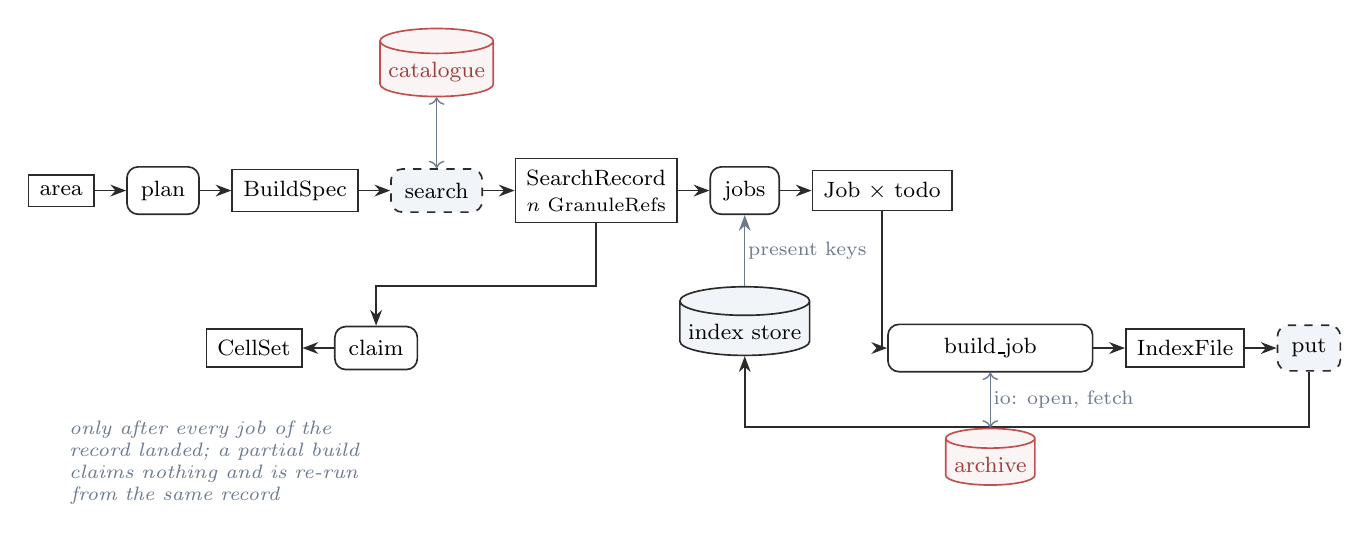
\begin{tikzpicture}[x=1mm,y=1mm, node distance=4mm]
  \node[val] (area) at (0,20) {area};
  \node[pure, right=of area] (plan) {plan};
  \node[val, right=of plan] (spec) {BuildSpec};
  \node[eff, right=of spec] (search) {search};
  \node[val, right=of search] (rec) {SearchRecord\\ \scriptsize $n$ GranuleRefs};
  \node[pure, right=of rec] (jobs) {jobs};
  \node[val, right=of jobs] (job) {Job $\times$ todo};
  \node[remote, above=9mm of search] (cmr) {catalogue};
  \draw[flow] (area) -- (plan); \draw[flow] (plan) -- (spec); \draw[flow] (spec) -- (search); \draw[flow] (search) -- (rec);
  \draw[flow] (rec) -- (jobs); \draw[flow] (jobs) -- (job);
  \draw[flowsoft, <->] (search) -- (cmr);
  \node[store, below=9mm of jobs] (store) {index store};
  \draw[flowsoft] (store) -- node[lblw, right] {present keys} (jobs);
  % second row
  \node[pure, minimum width=26mm] (bj) at (118,0) {build\_job};
  \node[val, right=of bj] (file) {IndexFile};
  \node[eff, right=of file] (put) {put};
  \draw[flow] (job.south) |- (bj.west);
  \draw[flow] (bj) -- (file); \draw[flow] (file) -- (put); \draw[flow] (put.south) |- ++(-6,-7) -| (store.south);
  \node[remote, below=7mm of bj] (s3) {archive};
  \draw[flowsoft, <->] (bj) -- node[lblw, right] {io: open, fetch} (s3);
  \node[pure] (claim) at (40,0) {claim};
  \node[val, left=of claim] (cells) {CellSet};
  \draw[flow] (rec.south) |- ++(0,-8) -| (claim.north);
  \draw[flow] (claim) -- (cells);
  \node[note, text width=40mm, anchor=north west] at (0,-8) {only after every job of the record landed; a partial
    build claims nothing and is re-run from the same record};
\end{tikzpicture}}
\caption{The build as stages over values. Rounded white boxes are pure; grey dashed boxes touch the catalogue, the
archive or the disk. The record of a search is the primary value: jobs, outcomes and the claim derive from it.}
\label{fig:buildstages}
\end{figure}

The values are small and frozen, and they are what crosses process boundaries:

\begin{lstlisting}
@dataclass(frozen=True, slots=True)
class GranuleRef:    # what a worker needs: strings, not the catalogue's object
    name: str; url: str; s3url: str; revision: str; native_id: str = ""

@dataclass(frozen=True, slots=True)
class BuildSpec:     # the ground at both resolutions; the shape the catalogue is asked
    collection: str; res: int; schema: str
    fine_cells: tuple[int, ...]; addressing: tuple[int, ...]
    ring: tuple[tuple[float, float], ...]; window: tuple[str, str] | None

@dataclass(frozen=True, slots=True)
class SearchRecord:  # PRIMARY, append-only: what the catalogue answered, when
    spec: BuildSpec; at: str; granules: tuple[GranuleRef, ...]

@dataclass(frozen=True, slots=True)
class Job:           # one granule under one spec; its key names the index file
    collection: str; granule: GranuleRef; res: int; schema: str; cellset_sha: str; params_sha: str
    @property
    def key(self) -> str: ...   # sha1(name, revision, schema, res, cellset, params)[:20]

@dataclass(frozen=True, slots=True)
class Outcome:
    key: str; rows: int; error: str | None
    seconds: float; requests: int; bytes: int
\end{lstlisting}

Three design points follow from writing it this way.

\textbf{The record is primary.} Today the catalogue's answer is cached for a day as a pickle of the client's
objects and the claim is a file mutated by each build. Storing \code{SearchRecord}s makes the claim a fold and
makes replay possible (Chapter~\ref{ch:replay}): a failed build is re-run from its record, not re-searched; what a
build \emph{would} do is computed from the record and the store's keys without touching the network.

\textbf{The job key names the file.} With content-addressed keys the resume set is a directory listing instead of
a footer read per file (33{,}484 reads today, before the first job starts), and the provenance question of
Chapter~\ref{ch:claim} is answered by the name: a file built under a different cell set has a different key. The
GPS collection stamps a metadata hash into its rows for the same reason; that is the \code{params\_sha} slot,
empty for the other five.

\textbf{Pure given io.} \code{build\_job} reads a remote file, so it is not pure in the strict sense; it is pure
\emph{given} two functions, \code{open} and \code{fetch}, passed in. In production they are the archive; in tests
they are a synthetic HDF5 file in memory. Nothing else in the stage touches the world, which is what makes it
testable per collection without a network and what lets a worker process run it with nothing but a \code{Job}.

\landed{\code{build.GranuleRef} (four strings plus a compatibility shim for the builders), \code{build.BuildCollection}
(the per-collection parameters), \code{build.run\_build} (the sequence, once, for ATL06, GEDI, GLAS, ICESSN and GPS)
over \code{pool.run\_pool}. Still proposed: \code{SearchRecord} stored, content-addressed keys, the claim as a fold.}

\section{Reading one granule}
\label{ch:readgranule}

Failure (c) of Chapter~\ref{ch:failures} does not disappear because the read happens once: the build still has to
find the chunk map and the positions inside a file whose structure is a tree of dependent reads. This chapter is
about paying that cost once as cheaply as possible.

The build's cost is in \code{build\_job}, and inside it almost entirely in reading the file's structure. Before
any position is read, the HDF5 library walks the superblock, the group tree and the chunk B-trees: for an ATL06
granule about 66 small reads, each a dependent round trip, because the next address is learned from the previous
read. Through a 1\,MiB block cache over the object store that walk took about 2\,s of a 3.3\,s granule; the position
fetch 0.5\,s; the actual computation 0.3\,s. Workers scaled the wall time until the machine ran out of threads to
wait on, and then not at all (Table~\ref{tab:workers}).

\begin{table}[h]
\footnotesize
\begin{tabular}{@{}rrrrl@{}}
\toprule
workers & wall (s) & granules/s & s per granule per worker & CPU busy \\
\midrule
4 & 81.0 & 1.23 & 3.24 & 20\,\% \\
8 & 41.9 & 2.39 & 3.35 & 44\,\% \\
16 & 26.2 & 3.81 & 4.20 & 80\,\% \\
32 & 26.2 & 3.81 & 8.39 & 92\,\% \\
\bottomrule
\end{tabular}
\caption{ATL06, 100 granules, 4 vCPU, before the whole-object read: latency-bound to 16 workers, then flat. The
per-granule time is the sum of serial round trips.}
\label{tab:workers}
\end{table}

A dependent walk cannot be parallelised, but it can be made local. The granule sizes decide how
(Figure~\ref{fig:timelines}):

\begin{itemize}
\item \textbf{Small granules (ATL06, GLAS, 2 to 128\,MB): read the whole object once.} The first 8\,MiB span is
  requested alone and the object's size read from the response's \code{Content-Range}, with no \code{HEAD} and no
  extra round trip; the remaining 8\,MiB spans go out in one concurrent submission; the structure walk then runs over
  an in-memory buffer at memory speed, and the position chunks are sliced from the same buffer. Objects over a cap
  (256\,MiB, since the per-worker peak is two to three times the object) fall back to the block cache having spent one
  span.
\item \textbf{Large granules (ATL03, 0.2 to 6.7\,GB): read bigger blocks.} The structure of an ATL03 file is
  clustered, so a 4\,MiB block satisfies the walk in 7 reads instead of 114 while moving 29\,MB instead of 120.
  Larger blocks read more for nothing (16\,MiB: 4 reads, 67\,MB, no faster).
\end{itemize}

\begin{figure}[tbp]
\wide{%
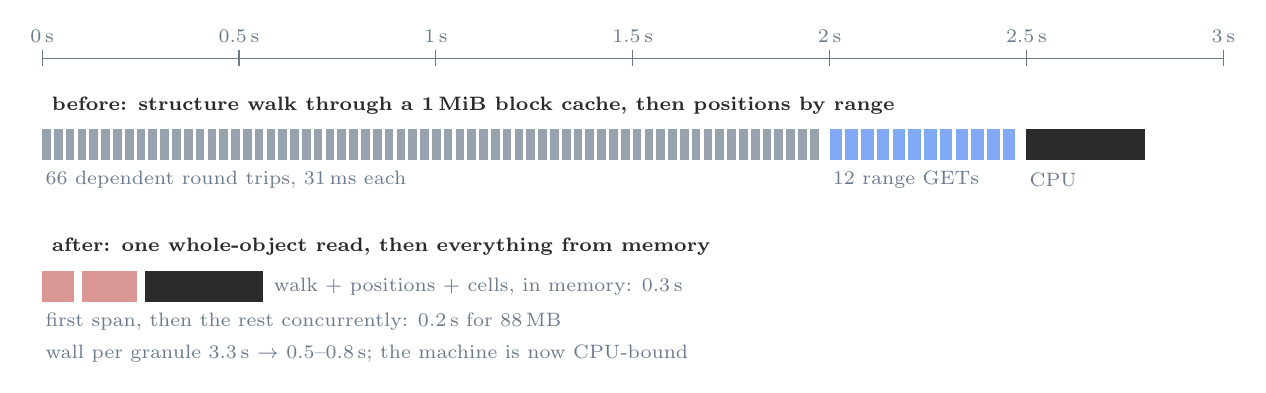
\begin{tikzpicture}[x=1mm,y=1mm]
  \draw[draw=soft, line width=0.4pt] (0,34) -- (150,34);
  \foreach \t in {0,0.5,...,3.0} {\draw[draw=soft, line width=0.4pt] ({\t*50},33) -- ({\t*50},35); \node[lbl, anchor=south] at ({\t*50},35.5) {\t\,s};}
  \node[hdr] at (0,28) {before: structure walk through a 1\,MiB block cache, then positions by range};
  \foreach \i in {0,...,65} {\fill[soft!70] ({\i*1.5},21) rectangle ({\i*1.5+1.1},25);}
  \foreach \i in {0,...,11} {\fill[idxblue!60] ({100+\i*2},21) rectangle ({100+\i*2+1.6},25);}
  \fill[ink] (125,21) rectangle (140,25);
  \node[lbl, anchor=west] at (0,18.5) {66 dependent round trips, 31\,ms each};
  \node[lbl, anchor=west] at (100,18.5) {12 range GETs};
  \node[lbl, anchor=west] at (125,18.5) {CPU};
  \node[hdr] at (0,10) {after: one whole-object read, then everything from memory};
  \fill[nasared!60] (0,3) rectangle (4,7); \fill[nasared!60] (5,3) rectangle (12,7);
  \fill[ink] (13,3) rectangle (28,7);
  \node[lbl, anchor=west] at (0,0.5) {first span, then the rest concurrently: 0.2\,s for 88\,MB};
  \node[lbl, anchor=west] at (29,5) {walk + positions + cells, in memory: 0.3\,s};
  \node[lbl, anchor=west] at (0,-3.5) {wall per granule 3.3\,s $\to$ 0.5--0.8\,s; the machine is now CPU-bound};
\end{tikzpicture}}
\caption{One ATL06 granule's build, before and after, on the same time axis. The serial walk disappears into a
buffer; what remains is computation, so adding workers past the core count buys nothing and the lever becomes
cores.}
\label{fig:timelines}
\end{figure}

Both cases go through one door. A \code{GranuleSource} is what a builder opens: \code{open()} returns the object
the HDF5 library parses (a memory buffer, or the block-cached remote file), \code{fetch(ranges)} returns byte ranges
from the \emph{same} bytes (sliced from the buffer, or range GETs), and \code{stats} counts what was moved. Every
dataset a builder reads goes through one function, \code{read\_via\_chunks}, which takes the dataset's chunk map
and asks the source for the chunks, decoding them with the same decoder the query uses. The builder therefore does
not know which path it is on, and a test can hand it a buffer of a synthetic file.

\begin{table}[h]
\footnotesize
\wide{\begin{tabular}{@{}llrrl@{}}
\toprule
collection & configuration & before & after & note \\
\midrule
ATL06, 100 granules, 8 workers & whole object & 44.7\,s & 21.3\,s & CPU 46\,\% $\to$ 94\,\% \\
ATL06, 300 granules, 6/8/12 workers & whole object & & 5.4 gran/s & flat in workers, CPU 92--98\,\% \\
ATL06, full regional rebuild (33\,484) & whole object & 3.9\,h & 62\,min & 9.1 gran/s sustained \\
GLAS, 35 granules, 8 workers & whole object & 7.4\,s & 4.1\,s & \\
GLAS, full rebuild (4\,799) & whole object & 10\,min & 3.5\,min & \\
ATL03, 20 granules, 8 workers & 4\,MiB blocks & 23.4\,s & 11.1\,s & 114 $\to$ 7 structure reads \\
ATL03, full regional rebuild (48\,838) & 4\,MiB, 16 workers & 12\,h & $\approx$7.3\,h & 1.88 gran/s, CPU-bound \\
\bottomrule
\end{tabular}}
\caption{Build measurements on the deployed instance (m6i.xlarge, 4 vCPU, in-region), 2026-10-17.}
\label{tab:buildnumbers}
\end{table}

The measurements (Table~\ref{tab:buildnumbers}) say the build is no longer waiting on the network. What is left
is computation in the worker, so the next lever is cores, not workers.\landed{\code{access.read\_whole\_object},
\code{GranuleSource}, \code{open\_granule}; \code{index.read\_via\_chunks}; \code{index.ATL03\_BLOCK\_SIZE = 4\,MiB}.
ATL06 and GLAS opt in to the whole object; GEDI stays on the block cache until its sizes are measured.}

\section{The build at runtime}
\label{ch:buildruntime}

The structural view says what is computed; this chapter says by whom. A build is one parent process and a pool of
worker processes (Figure~\ref{fig:buildproc}). The parent does everything that is cheap and must happen once:
plans the ground, logs in, searches the catalogue, lists the store, decides the jobs, and at the end claims and
folds the manifest. A worker does one thing: \code{build\_job} for the job it is handed, with its own login and its
own archive client.

\begin{figure}[tbp]
\wide{%
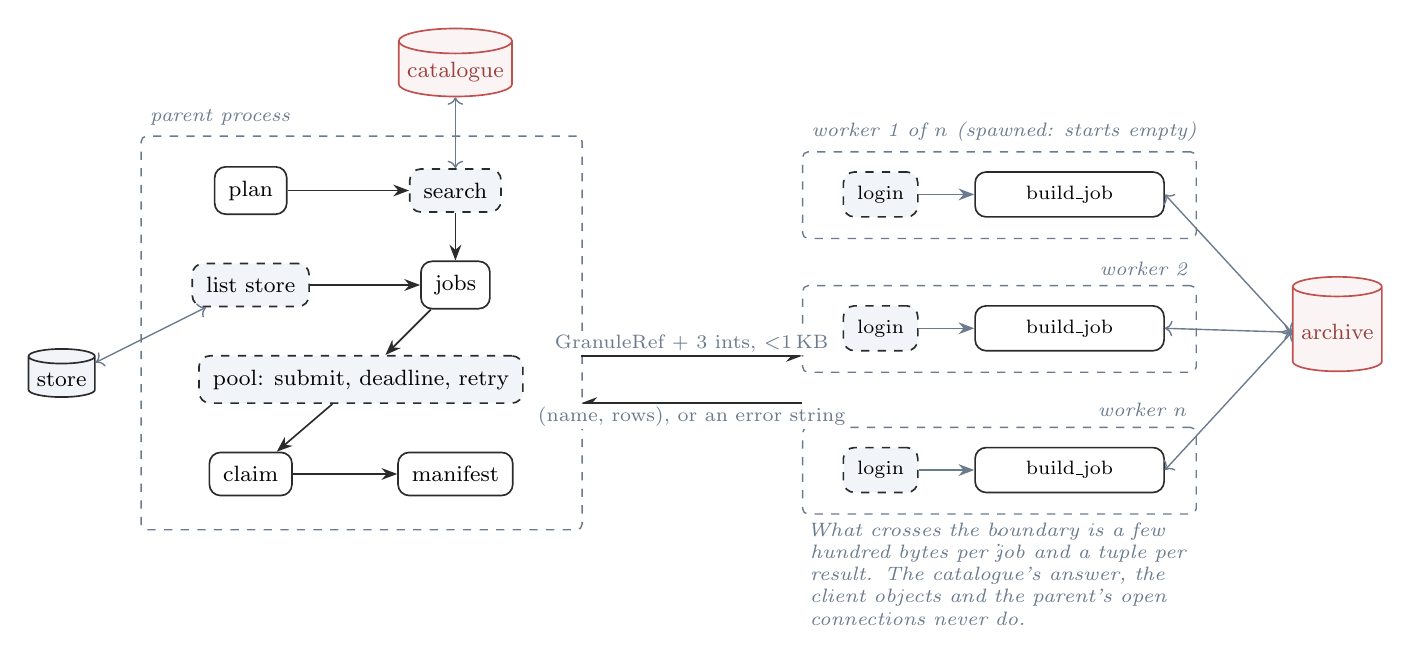
\begin{tikzpicture}[x=1mm,y=1mm]
  \node[proc, minimum width=56mm, minimum height=50mm, anchor=north west] (parent) at (0,50) {};
  \node[note, anchor=south west] at (parent.north west) {parent process};
  \node[pure] (plan) at (14,43) {plan};
  \node[eff] (search) at (40,43) {search};
  \node[eff] (list) at (14,31) {list store};
  \node[pure] (jobs) at (40,31) {jobs};
  \node[eff, minimum width=30mm] (pool) at (28,19) {pool: submit, deadline, retry};
  \node[pure] (claim) at (14,7) {claim};
  \node[pure] (man) at (40,7) {manifest};
  \draw[flow] (plan) -- (search); \draw[flow] (search) -- (jobs); \draw[flow] (list) -- (jobs);
  \draw[flow] (jobs) -- (pool); \draw[flow] (pool) -- (claim); \draw[flow] (claim) -- (man);
  % workers
  \foreach \i/\y in {0/48, 1/31, 2/13} {
    \node[proc, minimum width=50mm, minimum height=11mm, anchor=north west] (w\i) at (84,\y) {};
    \node[eff, font=\scriptsize] (login\i) at (94,{\y-5.5}) {login};
    \node[pure, font=\scriptsize, minimum width=24mm] (bj\i) at (118,{\y-5.5}) {build\_job};
    \draw[flowsoft] (login\i) -- (bj\i);
  }
  \node[note, anchor=south west] at (w0.north west) {worker 1 of $n$ (spawned: starts empty)};
  \node[note, anchor=south east] at (w1.north east) {worker 2};
  \node[note, anchor=south east] at (w2.north east) {worker $n$};
  \node[lbl] at (109,-1) {$\vdots$};
  \draw[flow] (56,22) -- node[lblw, above, pos=0.5] {GranuleRef + 3 ints, $<$1\,KB} (84,22);
  \draw[flow] (84,16) -- node[lblw, below, pos=0.5] {(name, rows), or an error string} (56,16);
  % archive
  \node[remote, minimum height=12mm] (s3) at (152,25) {archive};
  \foreach \i in {0,1,2} \draw[flowsoft, <->] (bj\i.east) -- (s3.west);
  \node[remote] (cmr) at (40,58) {catalogue};
  \draw[flowsoft, <->] (search) -- (cmr);
  \node[store] (store) at (-10,19) {store};
  \draw[flowsoft, <->] (list) -- (store);
  \node[note, text width=50mm, anchor=north west] at (84,2) {What crosses the boundary is a few hundred bytes per
    job and a tuple per result. The catalogue's answer, the client objects and the parent's open connections never
    do.};
\end{tikzpicture}}
\caption{The build at runtime. One parent, $n$ spawned workers, each holding its own archive client. The arrows
carry values small enough to pickle without thought.}
\label{fig:buildproc}
\end{figure}

\paragraph{Spawn, not fork.} A forked worker begins as a copy of its parent. For a regional ATL03 build the
parent holds the catalogue's answer, several gigabytes of client objects, and copy-on-write un-shares those pages
worker by worker until memory approaches $(n+1)$ times the parent; a 16-worker ATL06 build was killed that way. A
spawned worker begins empty and receives only its job. The price is a second of imports and a login per worker, paid
once per build.

\paragraph{One policy for the pool.} Five builders once owned five pools and disagreed on everything that matters.
The one pool now has one policy: submit every job; consume the futures \emph{in submission order} with a per-future
timeout computed from a monotonic clock (a laptop that sleeps must not report a healthy build as timed out), so a
progress callback sees jobs in a stable order; treat every worker exception as retryable, because the real cause of a
transient archive error is destroyed in transit when the error object cannot be pickled back; run a second attempt for
the failures in a fresh pool; then cancel what is left (Figure~\ref{fig:retry}).\landed{\code{pool.run\_pool}, called
with exactly \code{max\_workers} and \code{mp\_context}; \code{build.run\_build} claims only when every job of the
attempt landed and otherwise logs that it is not claiming.}

\begin{figure}[h]
\centering
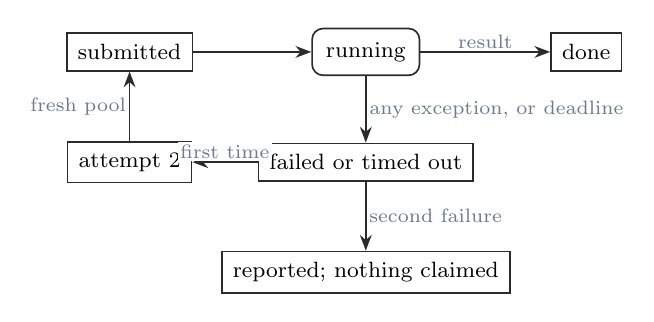
\begin{tikzpicture}[x=1mm,y=1mm]
  \node[val] (sub) at (0,0) {submitted};
  \node[pure] (run) at (30,0) {running};
  \node[val] (done) at (58,0) {done};
  \node[val] (fail) at (30,-14) {failed or timed out};
  \node[val] (retry) at (0,-14) {attempt 2};
  \node[val] (given) at (30,-28) {reported; nothing claimed};
  \draw[flow] (sub) -- (run); \draw[flow] (run) -- node[lblw, above] {result} (done);
  \draw[flow] (run) -- node[lblw, right] {any exception, or deadline} (fail);
  \draw[flow] (fail) -- node[lblw, above] {first time} (retry); \draw[flow] (retry) -- node[lblw, left] {fresh pool} (sub);
  \draw[flow] (fail) -- node[lblw, right] {second failure} (given);
\end{tikzpicture}
\caption{The life of one job in the pool. The claim at the end of the build requires every job to reach
\emph{done}; a single job in the bottom state withholds it, and the next run resumes from the files that landed.}
\label{fig:retry}
\end{figure}

\paragraph{How many workers.} After Chapter~\ref{ch:readgranule} an ATL06 granule costs about 0.7 core-seconds,
so on four vCPUs the knee is at six to eight workers and sixteen buys nothing but memory. The text collections and
ATL03 are still latency-bound (a whole-file GET, or a large structure walk) and take sixteen. Memory for sixteen
spawned workers with whole-object buffers peaked at 3.4\,GB on a 15\,GB machine; two collections are never built at
once.\landed{\code{BuildCollection.default\_workers}: 8 for the HDF5 builders, 16 for ATL03, ICESSN and GPS; GEDI's
per-granule timeout is 600\,s because a granule is a quarter orbit.}

%=====================================================================================================================
\clearpage

\part{From query specification to plan to execution}
\label{part:query}
%=====================================================================================================================

\section{The query specification}
\label{ch:queryspec}

Part~\ref{part:query} discharges \req{5}. Chapter~\ref{ch:queries} wrote the canonical queries as conjunctions of
area, time, filters and aggregation; the design's first move is to make that conjunction a value. A \code{Query}
names the collection, the area (a rectangle and, optionally, the polygon inside it), the window, the beam group
policy, and two flags (force a re-fetch; clip to cells rather than to the rectangle). It carries no derived state:
its cells, its catalogue of index rows and its split into what the lake has and what must be fetched are all
functions of it and of the stores, computed by the planner of the next chapter. Normalisation happens at the door:
a region name becomes its rectangle, a point and radius become a cell or a rectangle, a window becomes two
\code{YYYY-MM-DD} strings compared against the file-name clock. The per-mission filters of Table~\ref{tab:logical}
are not part of the query at all; they are the collection's, applied to decoded points, and the query can only
choose among the few policies the collection offers (which beam group; a confidence threshold for photons).

\section{The plan}
\label{ch:plan}

A query begins as a value: the area (a box, or a polygon inside it), the time window, the collection, and a few
flags (which beam groups, whether to force a re-fetch, whether to clip to cells). Turning it into points has a
planning half that touches only local stores and a fetching half that touches the archive. The planning half is
worth isolating because it is cheap, deterministic given the stores, and what every inspection tool (a dry run, a
byte-range map, a progress denominator) wants to see.

\begin{Verbatim}[fontsize=\footnotesize]
cells(query, grid)               -> tuple[int]       pure: addressing cells the area overlaps
scan(query, coll, store)         -> rows             EFFECT (DuckDB over the manifest-named index files)
have(coll, granules, lake)       -> set[ChunkKey]    EFFECT (the lake's key table): what is already decoded
plan_query(query, coll, rows, have) -> QueryPlan     pure: todo = chunks with any wanted cell not in have,
                                                           completed to whole beam groups, grouped by URL
render(plan)                     -> dict             pure: what the chunk map and the progress bar show
\end{Verbatim}

The scan asks the index for every row whose cell is wanted, restricted to the beam group and window, reading only
the files the manifest names. Rows arrive one per (granule, group, chunk, cell), each carrying its run. The plan
groups them by chunk: a chunk's wanted cells, its runs, one representative row for its byte ranges. Against the
lake's key table it splits chunks into \emph{have} (every wanted cell already decoded) and \emph{todo}
(Figure~\ref{fig:planset}). Two refinements are forced by later chapters and are decided here, not downstream:

\begin{itemize}
\item \textbf{A beam group is fetched whole.} If any beam of a group needs chunk $k$, the group's other beams'
  chunk $k$ join the todo set. Chapter~\ref{ch:lake} explains why the lake's file unit makes this necessary.
\item \textbf{Writes are narrowed to the wanted cells.} A chunk is far longer than a box and decodes points in
  cells the query never asked for. The plan records \code{want\_only}, the cells the lake may write; the rest of the
  strip is discarded (Chapter~\ref{ch:queryruntime} has the measurement that decided this).
\end{itemize}

\begin{figure}[tbp]
\wide{%
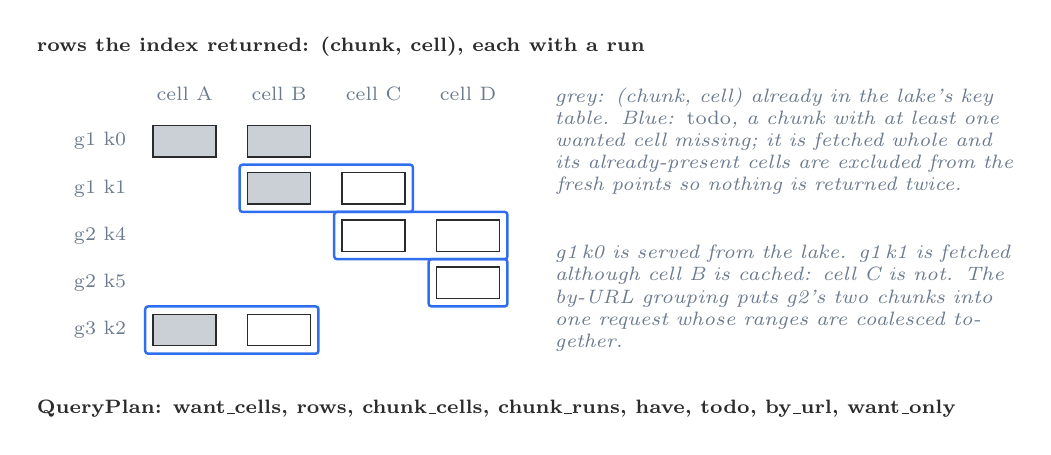
\begin{tikzpicture}[x=1mm,y=1mm]
  % grid: chunks x cells
  \node[hdr] at (0,44) {rows the index returned: (chunk, cell), each with a run};
  \foreach \c/\x in {A/20, B/32, C/44, D/56} {\node[lbl] at (\x,38) {cell \c};}
  \foreach \k/\y in {g1 k0/32, g1 k1/26, g2 k4/20, g2 k5/14, g3 k2/8} {\node[lbl, anchor=east] at (13,\y) {\k};}
  % cells present as rows
  \foreach \x/\y in {20/32, 32/32, 32/26, 44/26, 44/20, 56/20, 56/14, 20/8, 32/8} {\draw[draw=ink, line width=0.5pt] (\x-4,\y-2) rectangle (\x+4,\y+2);}
  % have (lake keys) shaded
  \foreach \x/\y in {20/32, 32/32, 32/26, 20/8} {\fill[soft!35] (\x-4,\y-2) rectangle (\x+4,\y+2);}
  \foreach \x/\y in {20/32, 32/32, 32/26, 20/8} {\draw[draw=ink, line width=0.5pt] (\x-4,\y-2) rectangle (\x+4,\y+2);}
  % todo chunks boxed
  \draw[draw=idxblue, line width=0.9pt, rounded corners=1pt] (27,23) rectangle (49,29);
  \draw[draw=idxblue, line width=0.9pt, rounded corners=1pt] (39,17) rectangle (61,23);
  \draw[draw=idxblue, line width=0.9pt, rounded corners=1pt] (51,11) rectangle (61,17);
  \draw[draw=idxblue, line width=0.9pt, rounded corners=1pt] (15,5) rectangle (37,11);
  \node[note, text width=58mm, anchor=north west] at (66,40) {grey: (chunk, cell) already in the lake's key table.
    Blue: \emph{todo}, a chunk with at least one wanted cell missing; it is fetched whole and its already-present
    cells are excluded from the fresh points so nothing is returned twice.};
  \node[note, text width=58mm, anchor=north west] at (66,20) {g1\,k0 is served from the lake. g1\,k1 is fetched
    although cell B is cached: cell C is not. The by-URL grouping puts g2's two chunks into one request whose ranges
    are coalesced together.};
  \node[hdr] at (0,-2) {QueryPlan: want\_cells, rows, chunk\_cells, chunk\_runs, have, todo, by\_url, want\_only};
\end{tikzpicture}}
\caption{The plan as a set picture. The lake's key table decides \emph{have}; a chunk goes to \emph{todo} if any
wanted cell of it is missing; todo is grouped by granule URL so one request per granule carries every range.}
\label{fig:planset}
\end{figure}

The plan is a value and should be serialisable as one: the query, the rows as an Arrow table, the have set and the
todo list. Chapter~\ref{ch:replay} uses that to replay an ingest without the planning half.\landed{\code{index\_atl06.plan\_bbox}
returns this dictionary without touching the network (keys \code{want\_cells}, \code{rows}, \code{chunk\_cells},
\code{chunk\_runs}, \code{chunk\_row}, \code{have}, \code{todo}, \code{n\_lake}, \code{by\_url}, \code{want\_only});
\code{\_whole\_groups} completes beam groups; the ATL03 planner does the same inline in \code{planner.\_ensure}.}

\begin{lstlisting}
@dataclass(frozen=True, slots=True)
class Query:
    collection: str; bbox: tuple[float, float, float, float]; polygon: tuple | None
    window: tuple[str, str] | None; res: int
    groups: tuple[str, ...] = ("strong",)       # beam groups wanted
    force: bool = False; clip_cells: bool = False

ChunkKey = tuple[str, str, int]                 # (granule, group member, chunk index)

@dataclass(frozen=True)
class QueryPlan:
    query: Query
    want_cells: tuple[int, ...]
    rows: pa.Table                              # one row per (chunk, cell), with its run
    have: frozenset[tuple[str, str, int, int]]  # (granule, beam, chunk, cell) in the lake
    todo: tuple[ChunkKey, ...]                  # whole beam groups
    by_url: Mapping[str, tuple[int, ...]]       # url -> row indices
    want_only: tuple[int, ...] | None
\end{lstlisting}

\section{Executing the plan: one chunk, step by step}
\label{ch:execute}

Execution is the same for every todo granule and, inside it, for every chunk. This chapter follows one chunk
through it and states, for each step, what the work is proportional to (Figure~\ref{fig:chunkflow}). The
distinction between per-point, per-chunk and per-granule work is the whole performance story of the query side:
anything per point must be native and vectorised, anything per chunk may be Python, anything per granule may be
a network round trip.

\begin{figure}[tbp]
\wide{%
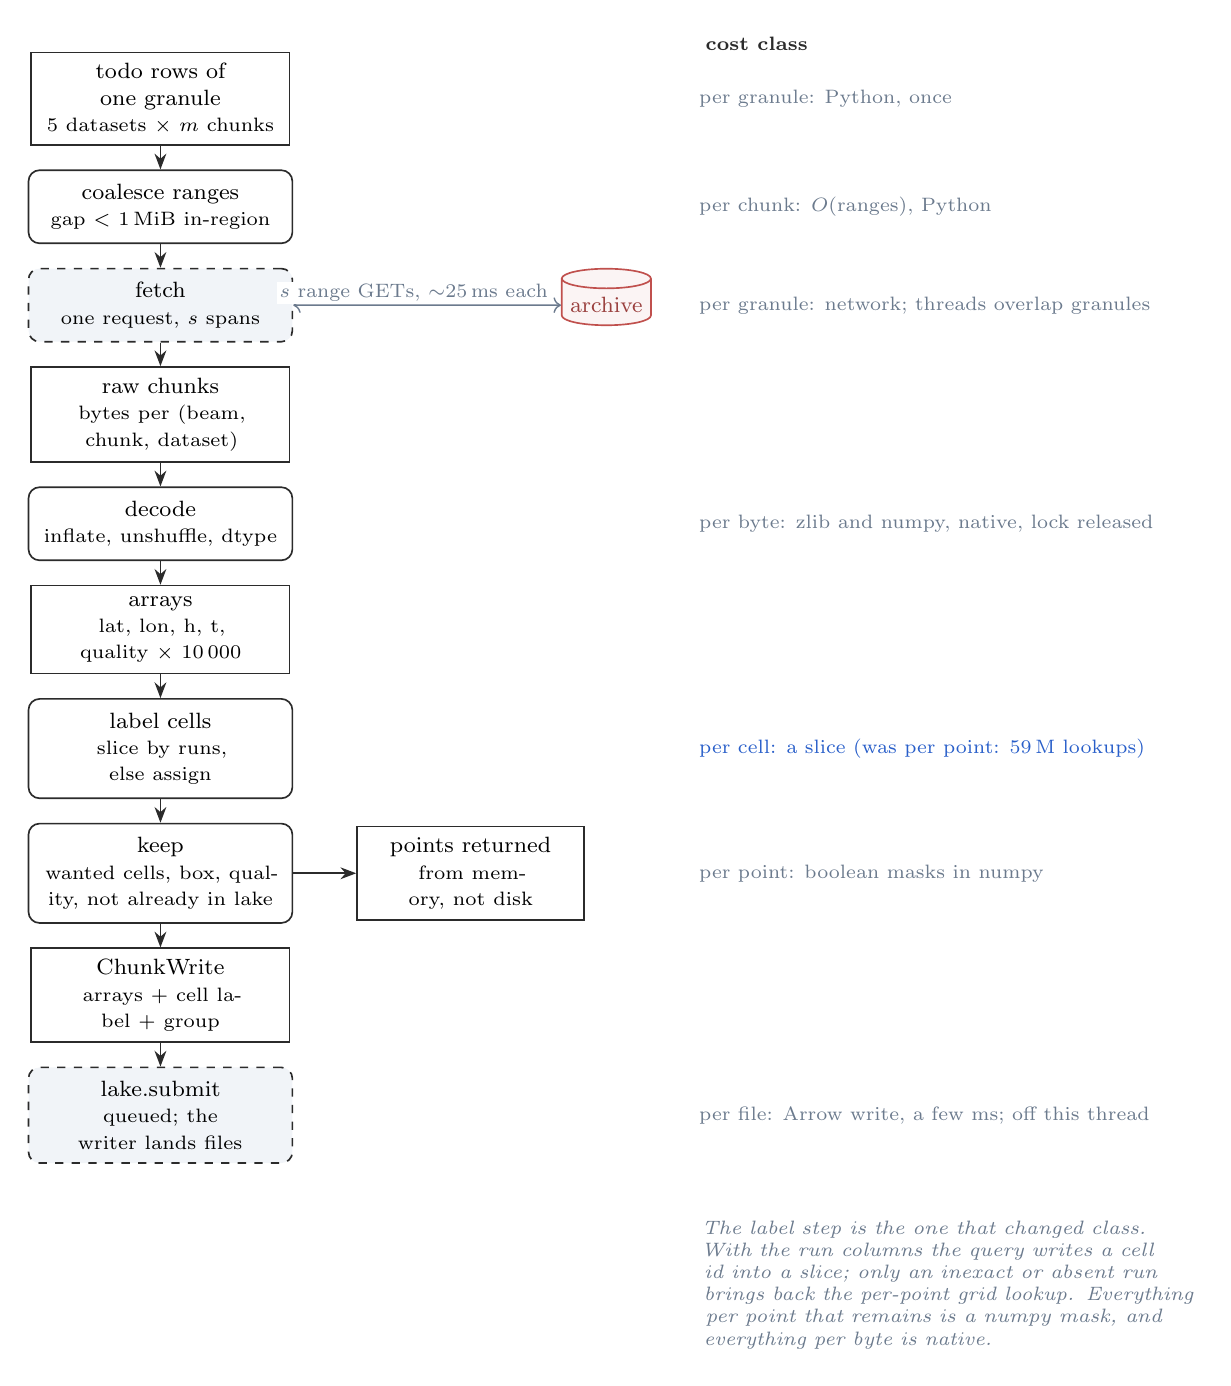
\begin{tikzpicture}[x=1mm,y=1mm, node distance=3mm]
  \node[val, text width=30mm] (rows) at (16,100) {todo rows of one granule\\ \scriptsize 5 datasets $\times$ $m$ chunks};
  \node[pure, text width=30mm, below=of rows] (coal) {coalesce ranges\\ \scriptsize gap $<$ 1\,MiB in-region};
  \node[eff, text width=30mm, below=of coal] (fetch) {fetch\\ \scriptsize one request, $s$ spans};
  \node[val, text width=30mm, below=of fetch] (raws) {raw chunks\\ \scriptsize bytes per (beam, chunk, dataset)};
  \node[pure, text width=30mm, below=of raws] (dec) {decode\\ \scriptsize inflate, unshuffle, dtype};
  \node[val, text width=30mm, below=of dec] (arr) {arrays\\ \scriptsize lat, lon, h, t, quality $\times$ 10\,000};
  \node[pure, text width=30mm, below=of arr] (lab) {label cells\\ \scriptsize slice by runs, else assign};
  \node[pure, text width=30mm, below=of lab] (keep) {keep\\ \scriptsize wanted cells, box, quality, not already in lake};
  \node[val, text width=30mm, below=of keep] (cw) {ChunkWrite\\ \scriptsize arrays + cell label + group};
  \node[eff, text width=30mm, below=of cw] (lake) {lake.submit\\ \scriptsize queued; the writer lands files};
  \node[val, text width=26mm, right=8mm of keep] (pts) {points returned\\ \scriptsize from memory, not disk};
  \foreach \a/\b in {rows/coal, coal/fetch, fetch/raws, raws/dec, dec/arr, arr/lab, lab/keep, keep/cw, cw/lake} {\draw[flow] (\a) -- (\b);}
  \draw[flow] (keep) -- (pts);
  \node[remote, right=34mm of fetch] (s3) {archive};
  \draw[flowsoft, <->] (fetch) -- node[lblw, above, pos=0.45] {$s$ range GETs, $\sim$25\,ms each} (s3);
  % cost column
  \node[hdr] at (84,107) {cost class};
  \node[lbl, anchor=west] at (rows.center -| 84,0) {per granule: Python, once};
  \node[lbl, anchor=west] at (coal.center -| 84,0) {per chunk: $O(\text{ranges})$, Python};
  \node[lbl, anchor=west] at (fetch.center -| 84,0) {per granule: network; threads overlap granules};
  \node[lbl, anchor=west] at (dec.center -| 84,0) {per byte: zlib and numpy, native, lock released};
  \node[lbl, anchor=west, text=idxblue!85!black] at (lab.center -| 84,0) {per cell: a slice (was per point: 59\,M lookups)};
  \node[lbl, anchor=west] at (keep.center -| 84,0) {per point: boolean masks in numpy};
  \node[lbl, anchor=west] at (lake.center -| 84,0) {per file: Arrow write, a few ms; off this thread};
  \node[note, text width=62mm, anchor=north west] at ([yshift=-6mm]lake.south -| 84,0) {The label step is the one that changed class. With
    the run columns the query writes a cell id into a slice; only an inexact or absent run brings back the
    per-point grid lookup. Everything per point that remains is a numpy mask, and everything per byte is native.};
\end{tikzpicture}}
\caption{One chunk through the executor, with the cost class of each step. The returned points come from memory;
the lake write is housekeeping for later queries and runs on other threads.}
\label{fig:chunkflow}
\end{figure}

\paragraph{Coalesce and fetch.} The granule's todo rows name $5 \times m$ byte ranges. Adjacent ranges separated
by less than a gap are merged into one span, because a request costs a round trip and bytes in the gap cost only
bandwidth; the gap is tuned by measurement to where the two balance (about 128\,KiB from outside the region, 1\,MiB
inside). One request per granule carries every span; granules are fetched on a thread pool sized for latency, not
cores, because a thread waiting on a GET uses no CPU.

\paragraph{Decode.} Each raw chunk is inflated, unshuffled and reinterpreted as its dtype. The three operations
release the interpreter lock and run at memory speed. The decoder is the same function the build used to read
positions, so a byte-identity test on one side covers the other.

\paragraph{Label.} This is where Chapter~\ref{ch:row} pays. For each wanted cell of the chunk the run is written
into a slice of a label array; a cell absent from the runs or with an inexact run sends the whole chunk to the
per-point assignment. ATL03 does the same with its edge columns and assigns only edge photons and outsiders.

\paragraph{Keep.} One predicate, applied once to the chunk's arrays as boolean masks: the label is a wanted cell;
the point lies inside the box (unless clipping to cells); the quality flag passes; and the cell is not one the lake
already returned for this chunk, so a partially cached chunk never contributes a cell twice. The kept points are the
answer; they are returned from memory and streamed to the caller granule by granule as each fetch lands.

\paragraph{Hand off.} The chunk's full arrays, the label and the beam group go into a \code{ChunkWrite} value and
onto the lake's queue. The executor does not write files, wait for them or know their names. One predicate, one
label, one value crossing to the writer: the five copies of this loop that exist today differ only in the
per-collection decode and quality functions, which are the slots of Chapter~\ref{ch:descriptor}.\landed{\code{index\_atl06.fetch\_bbox}
with its inner \code{\_ingest\_granule} and \code{\_keep}; \code{access.coalesce}, \code{decode\_chunk}, \code{unshuffle},
\code{map\_as\_completed}; the ATL03 path in \code{planner.\_process\_group}, \code{\_decode\_photons},
\code{\_materialize}. Five copies of the loop remain (ATL06, GLAS, GEDI, ICESSN, GPS) plus the ATL03 variant.}

%=====================================================================================================================
\clearpage
\part{The retrieval engine and the lake}
\label{part:lake}
%=====================================================================================================================

\section{The lake as a memo}
\label{ch:lake}

This part discharges \req{6}.

The lake is a cache of decoded points, partitioned by cell, read before any fetch and written after. Losing it costs
time, never truth: anything missing is re-fetched. Its design is dominated by one requirement, idempotence under
concurrency, and one measurement, the cost of a file.

\paragraph{Layout.} One Parquet file per (cell, granule, chunk, beam group), under a directory per cell:
\begin{Verbatim}[fontsize=\footnotesize]
lake/mission=ATL06/h3_cell=599686042/<granule stem>__strong__c12.parquet
lake/mission=ATL06/h3_cell=599686042/<granule stem>__weak__c12.parquet
lake/mission=GEDI/h3_cell=.../<stem>__full__c3.parquet        full / coverage power
lake/mission=ICESSN/h3_cell=.../<stem>__na__c0.parquet        beamless collections
\end{Verbatim}
Every point goes to the file of its \emph{own} cell, so a later query for a different sub-box of the same cell
re-filters correctly; a partial cell is impossible by construction. The cell directory is the unit of reads
(a query opens only the directories it asked for) and of eviction. A DuckDB table beside the lake records which
(granule, beam, chunk, cell) keys have landed; it is the \emph{have} of Chapter~\ref{ch:plan}.

\paragraph{Why a beam group.} The file count is the cost. Six files per (cell, chunk), one per beam, were 6{,}897
files for 2{,}960 chunks in one 8-cell ingest at 3 to 6\,ms each, and merging chunks of one beam was measured to be a
no-op because a scene box spans about one chunk per beam. Merging \emph{beams} cuts the count, but merging all six
is unsafe: the planner asks for the strong beams by default and for all six from the extraction API, so one name
per (cell, chunk) would be overwritten by whichever beam set came last. The group is the unit the planner requests
(\code{strong}, \code{weak}; \code{full}, \code{coverage}), so a group's file is always a full overwrite of a
deterministic name with the same content, whichever request produced it (Figure~\ref{fig:idem}). Six files became
two: 3{,}225 for the same ingest.

\begin{figure}[tbp]
\wide{%
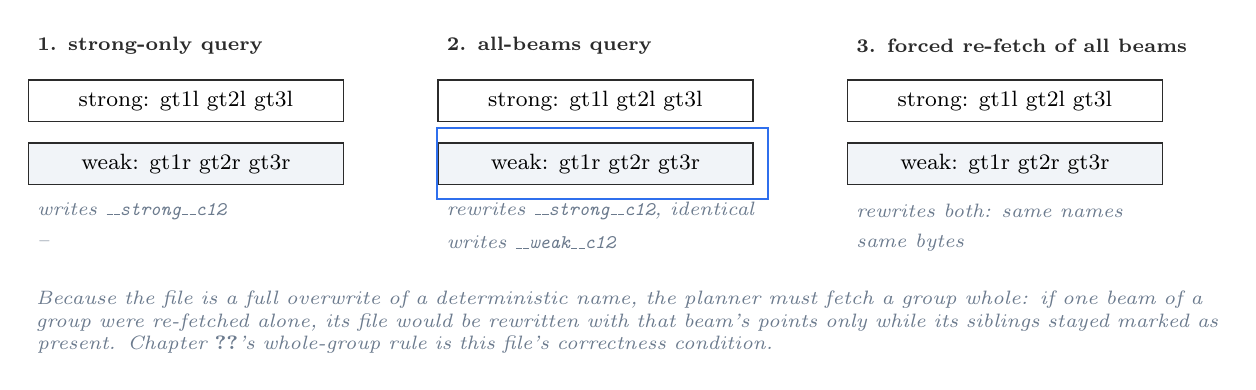
\begin{tikzpicture}[x=1mm,y=1mm]
  \node[hdr, anchor=west] at (0,20) {1. strong-only query};
  \node[val, minimum width=40mm, anchor=west] at (0,13) {strong: gt1l gt2l gt3l};
  \node[val, minimum width=40mm, anchor=west, fill=panel] at (0,5) {weak: gt1r gt2r gt3r};
  \node[note, anchor=west] at (0,-1) {writes \code{\_\_strong\_\_c12}};
  \node[note, anchor=west] at (0,-5) {--};
  \node[hdr, anchor=west] at (52,20) {2. all-beams query};
  \node[val, minimum width=40mm, anchor=west] at (52,13) {strong: gt1l gt2l gt3l};
  \node[val, minimum width=40mm, anchor=west, fill=panel] at (52,5) {weak: gt1r gt2r gt3r};
  \node[note, anchor=west] at (52,-1) {rewrites \code{\_\_strong\_\_c12}, identical};
  \node[note, anchor=west] at (52,-5) {writes \code{\_\_weak\_\_c12}};
  \node[hdr, anchor=west] at (104,20) {3. forced re-fetch of all beams};
  \node[val, minimum width=40mm, anchor=west] at (104,13) {strong: gt1l gt2l gt3l};
  \node[val, minimum width=40mm, anchor=west, fill=panel] at (104,5) {weak: gt1r gt2r gt3r};
  \node[note, anchor=west] at (104,-1) {rewrites both: same names};
  \node[note, anchor=west] at (104,-5) {same bytes};
  \draw[draw=idxblue, line width=0.9pt] (52,0.5) rectangle (94,9.5);
  \node[note, text width=150mm, anchor=north west] at (0,-10) {Because the file is a full overwrite of a deterministic
    name, the planner must fetch a group whole: if one beam of a group were re-fetched alone, its file would be
    rewritten with that beam's points only while its siblings stayed marked as present. Chapter~\ref{ch:plan}'s
    whole-group rule is this file's correctness condition.};
\end{tikzpicture}}
\caption{Idempotence across the two beam sets the planner can ask for. Each group's file has one name and one
content; nothing merges, nothing locks, nothing lists a directory.}
\label{fig:idem}
\end{figure}

\paragraph{One primitive.} Every lake file lands through one function: write to a temporary name in the same
directory, then rename. The rename is atomic, so a concurrent reader never sees a partial file; it creates or
replaces a directory entry, which is what the cell-statistics cache keys on; and it is the single place a test can
block, slow or fail to exercise ordering.

\paragraph{The writer.} Files are written by a small pool of threads fed by a bounded queue
(Figure~\ref{fig:writer}). The executor's threads block when the queue is full, so the fetch rate is throttled to
the write rate and memory stays bounded; this is why the writer is not made ``pure'' by handing writes back to the
caller as values, which would lose the backpressure. Two ordering rules are the contract: a key is marked present
only \emph{after} its file is on disk, so a crash loses cache and never truth; and a barrier exists that waits until
every queued write over a set of cells is on disk and marked, which the planner calls before reading \emph{have},
so a second query over the same area never reads a half-written lake. Marks are batched into one database
transaction per flush because opening the key table costs 150\,ms.

\begin{figure}[tbp]
\wide{%
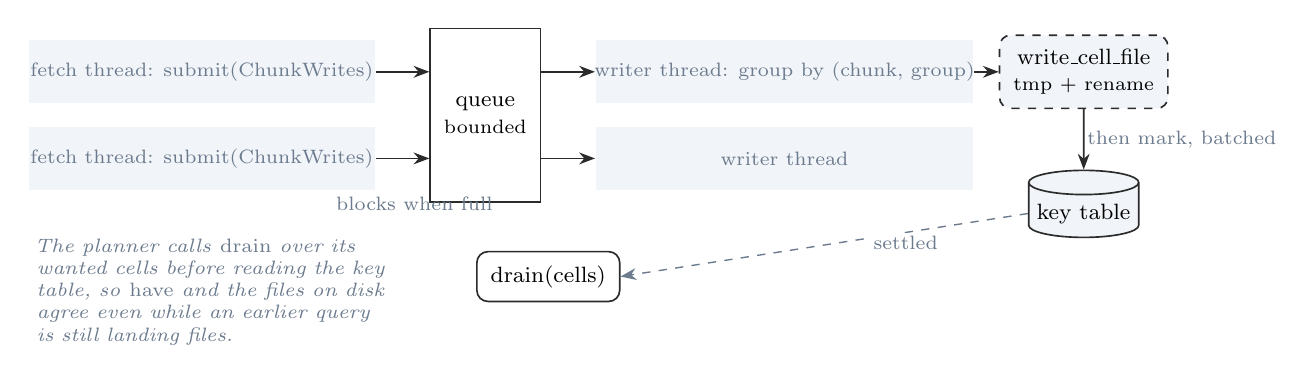
\begin{tikzpicture}[x=1mm,y=1mm]
  \node[lane, minimum width=44mm, minimum height=8mm] (f1) at (22,30) {}; \node[lbl] at (22,30) {fetch thread: submit(ChunkWrites)};
  \node[lane, minimum width=44mm, minimum height=8mm] (f2) at (22,19) {}; \node[lbl] at (22,19) {fetch thread: submit(ChunkWrites)};
  \node[val, minimum height=22mm, minimum width=14mm] (q) at (58,24.5) {queue\\ \scriptsize bounded};
  \draw[flow] (f1.east) -- (q.west |- f1.east); \draw[flow] (f2.east) -- (q.west |- f2.east);
  \node[lbl, anchor=north] at (49,14.5) {blocks when full};
  \node[lane, minimum width=48mm, minimum height=8mm] (w1) at (96,30) {}; \node[lbl] at (96,30) {writer thread: group by (chunk, group)};
  \node[lane, minimum width=48mm, minimum height=8mm] (w2) at (96,19) {}; \node[lbl] at (96,19) {writer thread};
  \draw[flow] (q.east |- w1.west) -- (w1.west); \draw[flow] (q.east |- w2.west) -- (w2.west);
  \node[eff] (file) at (134,30) {write\_cell\_file\\ \scriptsize tmp + rename};
  \draw[flow] (w1.east) -- (file);
  \node[store] (meta) at (134,12) {key table};
  \draw[flow] (file) -- node[lblw, right] {then mark, batched} (meta);
  \node[pure] (drain) at (66,4) {drain(cells)};
  \draw[flowsoft, dashed] (meta.west) -- node[lblw, below, pos=0.3] {settled} (drain.east);
  \node[note, text width=44mm, anchor=north west] at (0,10) {The planner calls \emph{drain} over its wanted cells
    before reading the key table, so \emph{have} and the files on disk agree even while an earlier query is still
    landing files.};
\end{tikzpicture}}
\caption{The writer. A bounded queue gives backpressure; marking after landing gives crash safety; the drain barrier
gives read-after-write consistency to the next plan.}
\label{fig:writer}
\end{figure}

\paragraph{Failure unit.} A group's chunk may touch several cells, and one cell's file may fail. The write returns,
per cell, whether its file landed; the writer marks every beam of the group present in the cells that landed and in
none of the cells that failed, so the chunk is re-fetched there rather than believed. Cells with no valid points are
marked too, or an all-fill cell would be re-fetched forever.

\paragraph{Eviction.} The lake has a byte budget per mission and globally. Eviction is by cell directory, least
recently used, protecting the cells of the query in flight, and runs off the request thread. The cell statistics it
needs are cached per directory and invalidated by the directory's modification time, which the rename
updates.\landed{\code{lake.write\_cell\_file}, \code{write\_chunk\_group} (returns \code{\{cell: landed\}}),
\code{ChunkWrite.group}, \code{\_Writer} with \code{submit}/\code{drain}/\code{\_flush}, \code{mark\_ingested\_many},
\code{ingested\_chunk\_cells}; \code{meta.duckdb} beside the index. ATL03 photons still write inline from their
worker processes via \code{write\_photons}.}

\section{What reads the lake}
\label{ch:lakereaders}

The lake is the system's contract with analysis (Figure~\ref{fig:lakereaders}). Every query of
Chapter~\ref{ch:queries} beyond Q1 is arithmetic over lake files: the coverage survey (Q2) counts passes, days and
years per cell from the lake's key table and the index manifest without touching the archive; co-registration (Q3)
reads two sources' cells, converts each to a common frame and epoch with the conversions of
Chapter~\ref{ch:logical}, and pairs points within 35\,m; the per-cell time series (Q4) reads every source's cells at
resolution 8, fits its fixed-effects surface and reports window medians and a trend; the lake-level and profile
tools (Q5) read a thin polygon's cells per pass. None of them knows a byte range, a chunk or a granule; they know a
table of positions, heights, times and a cell column, per source, with the source's native height and the
quality filter already applied. That is why the index and the lake share one resolution: the cell a row was
addressed by is the cell its points are filed under, and an analysis that asks for a cell gets exactly the points
the index promised.

\begin{figure}[tbp]
\wide{%
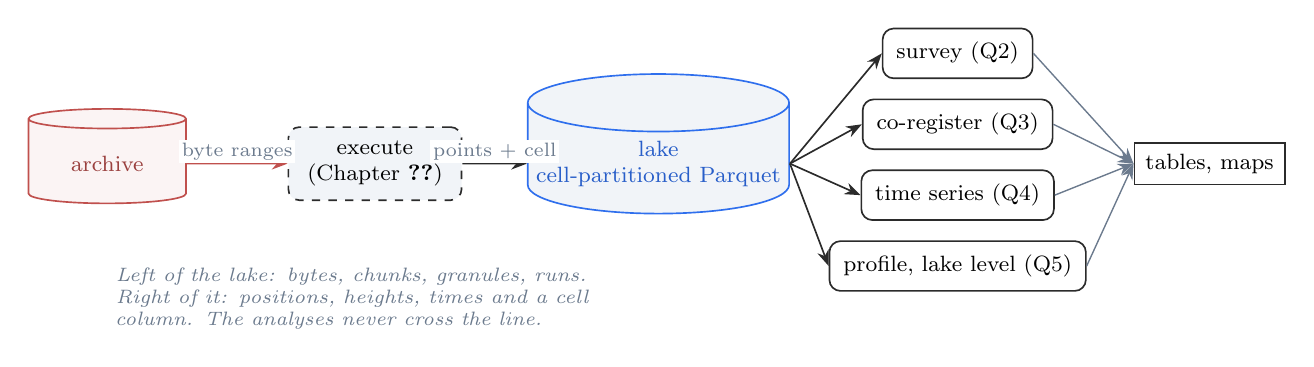
\begin{tikzpicture}[x=1mm,y=1mm]
  \node[remote, minimum width=20mm, minimum height=12mm] (s3) at (0,10) {archive};
  \node[eff, minimum width=22mm] (eng) at (34,10) {execute\\(Chapter~\ref{ch:execute})};
  \node[store, minimum width=24mm, minimum height=14mm, acc] (lake) at (70,10) {lake\\\footnotesize cell-partitioned Parquet};
  \node[pure] (q2) at (108,24) {survey (Q2)};
  \node[pure] (q3) at (108,15) {co-register (Q3)};
  \node[pure] (q4) at (108,6) {time series (Q4)};
  \node[pure] (q5) at (108,-3) {profile, lake level (Q5)};
  \node[val] (ui) at (140,10) {tables, maps};
  \draw[flow, draw=nasared] (s3) -- node[lblw, above] {byte ranges} (eng);
  \draw[flow] (eng) -- node[lblw, above] {points + cell} (lake);
  \foreach \q in {q2,q3,q4,q5} { \draw[flow] (lake.east) -- (\q.west); \draw[flowsoft] (\q.east) -- (ui.west); }
  \node[note, text width=60mm, anchor=north west] at (0,-2) {Left of the lake: bytes, chunks, granules, runs.
    Right of it: positions, heights, times and a cell column. The analyses never cross the line.};
\end{tikzpicture}}
\caption{The lake between the retrieval engine and the analyses. Everything to its right is pure arithmetic over
cell files; everything to its left is the machinery of Parts~IV--VI.}
\label{fig:lakereaders}
\end{figure}

\section{The query at runtime}
\label{ch:queryruntime}

Four kinds of thread and one kind of process take part in a query (Figure~\ref{fig:lanes}). The request thread
plans, reads the lake, and streams results to the caller as they arrive. A pool of fetch threads runs the executor
of Chapter~\ref{ch:execute}, one granule per task; it is sized for latency (up to 16) because its threads wait.
The writer threads land files. For ATL03 only, decoding and the co-registration of 100{,}000 photons per chunk is
CPU work heavy enough to be sent to spawned worker processes, one per (granule, beam) group, which fetch, decode,
assign and write their own files and return the key set for the parent to mark.

\begin{figure}[tbp]
\wide{%
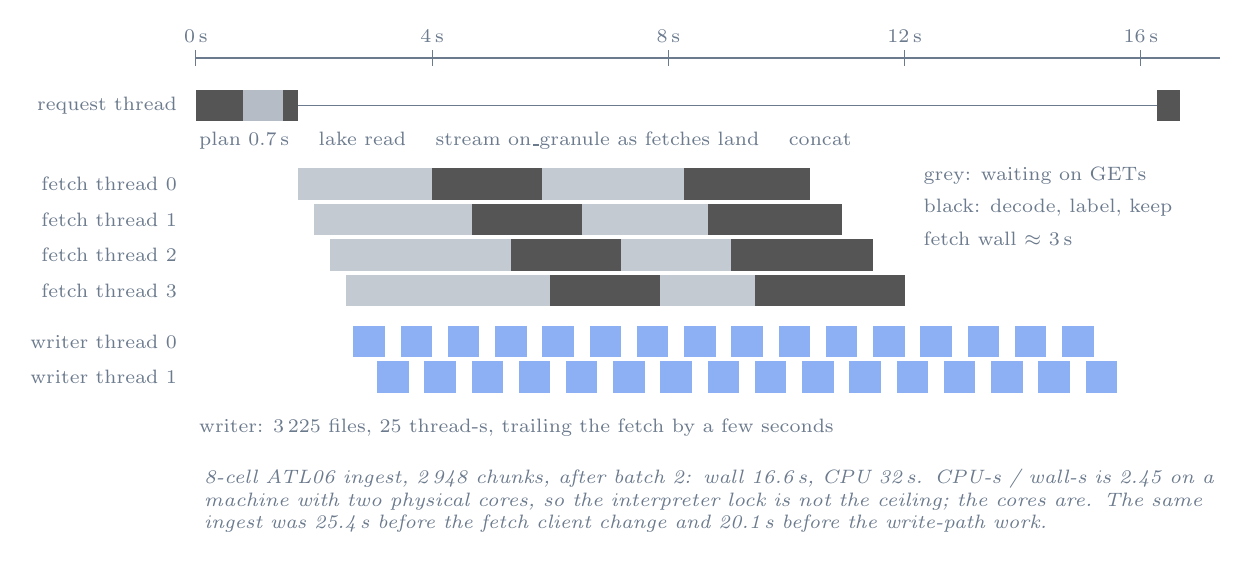
\begin{tikzpicture}[x=1mm,y=1mm]
  \draw[draw=soft, line width=0.4pt] (30,46) -- (160,46);
  \foreach \t in {0,4,...,16} {\draw[draw=soft, line width=0.4pt] ({30+\t*7.5},45) -- ({30+\t*7.5},47); \node[lbl, anchor=south] at ({30+\t*7.5},47.5) {\t\,s};}
  \node[lbl, anchor=east] at (28,40) {request thread};
  \fill[ink!80] (30,38) rectangle (36,42); \node[lbl, anchor=west, text=white] at (30,40) {};
  \fill[soft!50] (36,38) rectangle (41,42);
  \fill[ink!80] (41,38) rectangle (43,42);
  \draw[draw=soft, line width=0.4pt] (43,40) -- (152,40);
  \fill[ink!80] (152,38) rectangle (155,42);
  \node[lbl, anchor=west] at (30,35.5) {plan 0.7\,s \quad lake read \quad stream on\_granule as fetches land \quad concat};
  \foreach \i in {0,...,3} {
    \node[lbl, anchor=east] at (28,{30-4.5*\i}) {fetch thread \i};
    \fill[soft!40] ({43+\i*2},{28-4.5*\i}) rectangle ({60+\i*5},{32-4.5*\i});
    \fill[ink!80] ({60+\i*5},{28-4.5*\i}) rectangle ({74+\i*5},{32-4.5*\i});
    \fill[soft!40] ({74+\i*5},{28-4.5*\i}) rectangle ({92+\i*3},{32-4.5*\i});
    \fill[ink!80] ({92+\i*3},{28-4.5*\i}) rectangle ({108+\i*4},{32-4.5*\i});
  }
  \node[lbl, anchor=west] at (122,31) {grey: waiting on GETs};
  \node[lbl, anchor=west] at (122,27) {black: decode, label, keep};
  \node[lbl, anchor=west] at (122,23) {fetch wall $\approx$ 3\,s};
  \foreach \i in {0,1} {
    \node[lbl, anchor=east] at (28,{10-4.5*\i}) {writer thread \i};
    \foreach \x in {50,56,...,140} {\fill[idxblue!55] ({\x+\i*3},{8-4.5*\i}) rectangle ({\x+4+\i*3},{12-4.5*\i});}
  }
  \node[lbl, anchor=west] at (30,-1) {writer: 3\,225 files, 25 thread-s, trailing the fetch by a few seconds};
  \node[note, text width=128mm, anchor=north west] at (30,-5) {8-cell ATL06 ingest, 2\,948 chunks, after batch 2:
    wall 16.6\,s, CPU 32\,s. CPU-s / wall-s is 2.45 on a machine with two physical cores, so the interpreter lock is
    not the ceiling; the cores are. The same ingest was 25.4\,s before the fetch client change and 20.1\,s before the
    write-path work.};
\end{tikzpicture}}
\caption{One query's threads over time. Fetch threads alternate between waiting and decoding; the writer trails;
the request thread streams each granule's points as its fetch lands rather than after the slowest.}
\label{fig:lanes}
\end{figure}

\paragraph{Where the time goes, and what it rules out.} Fetch wall is about 3\,s for a scene: the archive client
sustains 670 to 840\,MB/s in-region and the request count is set by coalescing. The rest is CPU: decode, the
remaining per-point masks, Arrow writes. The ratio of CPU-seconds to wall-seconds is 2.45 on two physical cores,
which answers the question that always comes next. A process pool for decode and write would only help if the
interpreter lock were serialising the threads, which would show as a ratio near 1.0 with wall well above fetch; at
2.45 the threads already overlap and the machine is simply out of cores. The ATL03 process pool is justified by its
heavier per-chunk CPU, and it is spawned, not forked, because it runs inside a web server that holds a live archive
client, an event loop and the writer's threads, none of which survive a fork intact.

\paragraph{What was measured not to help.} Pre-caching the cells adjacent to the request (writing the whole decoded
strip rather than the wanted cells) was tested twice. It made the first query 1.9 to 2.1 times slower and the
neighbouring query slower too, because a chunk is re-fetched if \emph{any} wanted cell is missing and the strip only
brushes the neighbour. Raising the archive client's connection pool did nothing: the throughput cap is the machine's.
Both results are recorded where the knobs live so the hypotheses are not re-tested by
accident.\landed{\code{access.map\_as\_completed} (completion-order streaming), \code{FETCH\_WORKER\_CAP = 16},
\code{lake.\_Writer}, \code{planner.\_ensure} with a spawn \code{ProcessPoolExecutor}; the measurements in the
\code{precache\_adjacent} and \code{open\_granule} docstrings and in \code{scripts/bench\_ingest\_phases.py}.}

%=====================================================================================================================
\clearpage

\clearpage
\part{The framework}
\label{part:framework}
%=====================================================================================================================

\section{The collection descriptor}
\label{ch:descriptor}

Parts~\ref{part:build}--\ref{part:lake} described one build and one query, and this chapter discharges \req{7}. Today there are six of each, and they differ in exactly the
ways Table~\ref{tab:collections} listed: how a file's structure maps to element intervals, where positions come
from, how a chunk is decoded into points, what quality means, which group a beam belongs to. Everything else (the
driver, the pool, the resume set, the claim, the plan, the executor's loop, the keep predicate, the writer) is the
same sequence written several times with those differences inlined. The framework is the step of making the
differences a \emph{value}, the \code{Collection} descriptor, and the sequence a single implementation that reads
the value where it needs to (Figure~\ref{fig:plugboard}).

\begin{lstlisting}
@dataclass(frozen=True, slots=True)
class Dataset:
    key: str            # index-row and points column name
    path: str           # HDF5 path relative to the group, or a CSV field index
    role: str = ""      # "lat" | "lon" | "h" | "t" | "quality" | ""

@dataclass(frozen=True, slots=True)
class HDF5Chunked:      # ATL03, ATL06, GLAS: one chunk map per group
    groups: tuple[str, ...]          # beams; ("",) for GLAS
    reference: str                   # the dataset whose chunking is the group's
    positions: Callable              # (group, datasets, fetch) -> Positions
    group_scalars: Callable | None   # (file) -> {"sc_orient", "sdp_epoch"}

@dataclass(frozen=True, slots=True)
class HDF5Spans:        # GEDI: rows are spans at the union of boundaries
    groups: tuple[str, ...]; positions: Callable; quality_field: Callable

@dataclass(frozen=True, slots=True)
class TextLines:        # ICESSN, GPS: rows are line byte spans per cell
    scan: Callable      # (bytes) -> LineScan(lat, lon, start, end)
    header_in_rows: bool

@dataclass(frozen=True, slots=True)
class Collection:
    key: str; mission: str; short_name: str; version: str
    res: int; schema: str
    window: tuple[str, str] | None
    layout: HDF5Chunked | HDF5Spans | TextLines
    datasets: tuple[Dataset, ...]
    parse_name: Callable[[str], dict]           # orbit numbers and dates from the name
    date_of: Callable[[str, dict], str]         # "YYYYMMDD" for window and manifest
    decode: Callable                            # (raws, row) -> Points, pre-mask
    quality: Callable | None                    # (Points) -> bool mask
    groups_of: Callable[[dict], Mapping[str, str]]   # beam -> "strong" | "weak" ...
    row_extras: tuple[str, ...] = ()            # extra index columns (GPS geometry)
    point_extras: tuple[str, ...] = ()          # extra lake columns ("quality", ...)
    job_params: Callable | None = None          # (record, io) -> (params, sha); GPS
\end{lstlisting}

Every function-valued field is a module-level function, so the descriptor pickles across a spawn boundary as a
name and a worker looks it up in a registry. Presentation (labels, colours, default selection) is not in the
descriptor; it is an application table keyed by \code{Collection.key}, because the framework never draws anything.

\begin{figure}[tbp]
\wide{%
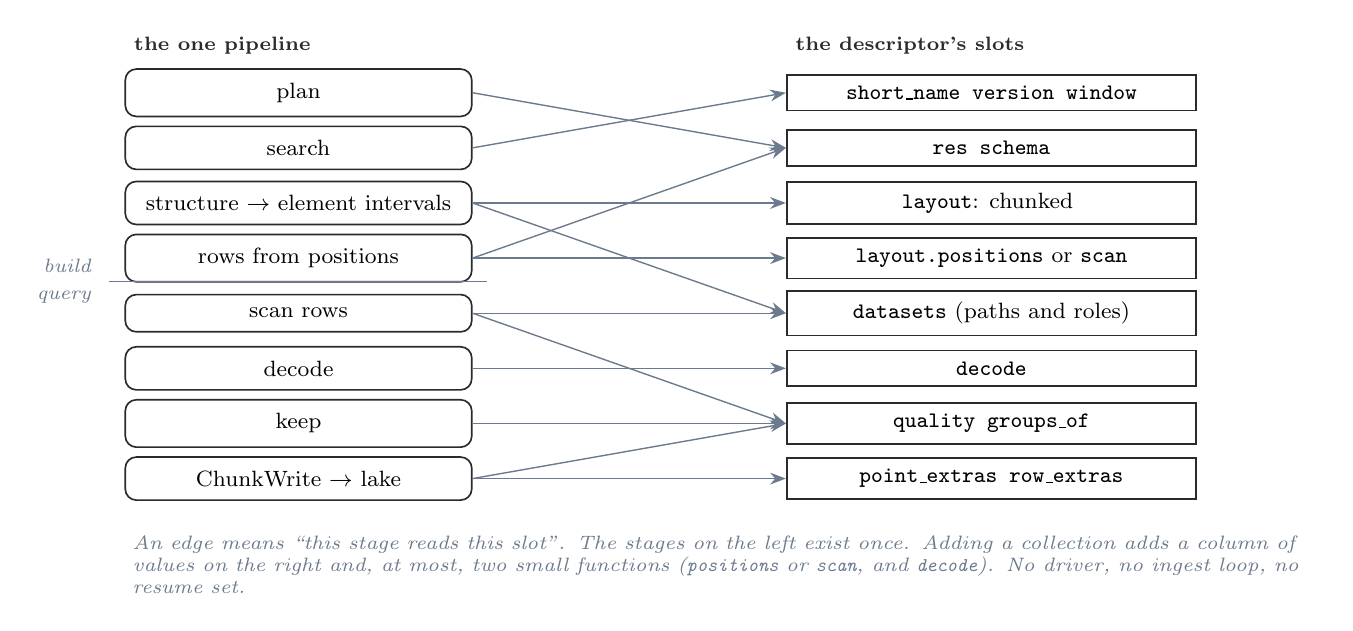
\begin{tikzpicture}[x=1mm,y=1mm]
  \node[hdr] at (0,74) {the one pipeline};
  \foreach \n/\y/\t in {plan/68/plan, search/61/search, structure/54/structure $\to$ element intervals, rows/47/rows from positions, scan/40/scan rows, exec/33/decode, keep/26/keep, write/19/ChunkWrite $\to$ lake} {
    \node[pure, anchor=west, minimum width=44mm] (\n) at (0,\y) {\t};
  }
  \draw[draw=soft, line width=0.4pt] (-2,44) -- (46,44); \node[note, anchor=east] at (-3,46) {build};
  \node[note, anchor=east] at (-3,42) {query};
  \node[hdr] at (84,74) {the descriptor's slots};
  \foreach \n/\y/\t in {sn/68/\code{short\_name}\, \code{version}\, \code{window}, res/61/\code{res}\, \code{schema}, lay/54/\code{layout}: chunked / spans / lines, pos/47/\code{layout.positions} or \code{scan}, ds/40/\code{datasets} (paths and roles), dec/33/\code{decode}, q/26/\code{quality}\, \code{groups\_of}, ex/19/\code{point\_extras}\, \code{row\_extras}} {
    \node[val, anchor=west, minimum width=52mm] (\n) at (84,\y) {\t};
  }
  \draw[flowsoft] (plan.east) -- (res.west);
  \draw[flowsoft] (search.east) -- (sn.west);
  \draw[flowsoft] (structure.east) -- (lay.west);
  \draw[flowsoft] (structure.east) -- (ds.west);
  \draw[flowsoft] (rows.east) -- (pos.west);
  \draw[flowsoft] (rows.east) -- (res.west);
  \draw[flowsoft] (scan.east) -- (ds.west);
  \draw[flowsoft] (scan.east) -- (q.west);
  \draw[flowsoft] (exec.east) -- (dec.west);
  \draw[flowsoft] (keep.east) -- (q.west);
  \draw[flowsoft] (write.east) -- (ex.west);
  \draw[flowsoft] (write.east) -- (q.west);
  \node[note, text width=150mm, anchor=north west] at (0,13) {An edge means ``this stage reads this slot''. The
    stages on the left exist once. Adding a collection adds a column of values on the right and, at most, two small
    functions (\code{positions} or \code{scan}, and \code{decode}). No driver, no ingest loop, no resume set.};
\end{tikzpicture}}
\caption{The plug board: which stage of the one pipeline consults which slot of a collection's descriptor. This is
the structural meaning of ``pluggable''.}
\label{fig:plugboard}
\end{figure}

\paragraph{Two descriptors, written out.} ATL06, the reference HDF5 collection:

\begin{lstlisting}
ATL06 = Collection(
    key="ATL06", mission="ATL06", short_name="ATL06", version="007", res=5, schema="atl06-3",
    window=("2018-10-01", "2027-01-01"),
    layout=HDF5Chunked(groups=("gt1l","gt1r","gt2l","gt2r","gt3l","gt3r"), reference="latitude",
        positions=slots.positions_identity,      # lat/lon per element
        group_scalars=slots.icesat2_scalars),    # sc_orient, sdp epoch
    datasets=(Dataset("latitude", "land_ice_segments/latitude", "lat"),
              Dataset("longitude", "land_ice_segments/longitude", "lon"),
              Dataset("h_li", "land_ice_segments/h_li", "h"),
              Dataset("delta_time", "land_ice_segments/delta_time", "t"),
              Dataset("atl06_quality_summary", "land_ice_segments/atl06_quality_summary",
                      "quality")),
    parse_name=slots.parse_icesat2_name, date_of=slots.date_from_name,
    decode=slots.decode_shared_chunk, quality=slots.quality_equals_zero,
    groups_of=slots.icesat2_strong_weak, point_extras=("quality",),
)
\end{lstlisting}

ICESSN, a text collection:

\begin{lstlisting}
ICESSN = Collection(
    key="ICESSN", mission="ICESSN", short_name="ILATM2", version="2", res=5, schema="icessn-4",
    window=None, layout=TextLines(scan=icessn.scan_lines, header_in_rows=False),
    datasets=(), parse_name=icessn.parse_name, date_of=slots.date_from_name,
    row_extras=("itrf_year",), decode=icessn.parse_span_points, quality=None,
    groups_of=slots.no_groups,
    point_extras=("sn_slope", "we_slope", "itrf_year"),
)
\end{lstlisting}

GPS differs from ICESSN in four fields: \code{header\_in\_rows=True}, five row extras carrying the sled geometry,
a \code{job\_params} that reads the traverse-metadata granule once in the parent and hashes it, and its own
\code{decode}. The same pattern that stamps a parameter hash into a job key (Chapter~\ref{ch:buildvalues}) is what
makes a metadata change invalidate the right files.

\paragraph{Where today's code goes.} The per-collection functions that exist today become the slots; nothing is
rewritten, only moved and given a signature (Table~\ref{tab:slots}).\landed{\code{build.BuildCollection} is the
build half of this descriptor (key, short name, version, resolution, index directory, resume set, timeout,
workers, prepare); \code{coverage.collections()} holds the presentation half. The query half and the layout kinds
are proposed.}

\begin{table}[h]
\footnotesize
\begin{tabular}{@{}lp{70mm}@{}}
\toprule
slot & existing code \\
\midrule
\code{positions} (ATL03) & the segment-to-photon mapping in the ATL03 builder \\
\code{positions\_identity} & ATL06 and GLAS position reads via \code{read\_via\_chunks} \\
\code{HDF5Spans} cutting & \code{index\_gedi.chunk\_spans}, \code{chunk\_of}, \code{span\_offset} (already pure) \\
\code{TextLines.scan} & \code{index\_icessn.\_parse\_fields} and its loop; the GPS equivalents \\
\code{decode} & \code{index\_atl06.\_decode\_chunk}, \code{index\_glas.\_decode\_chunk}, \code{index\_gedi.\_decode\_span}, \code{planner.\_decode\_photons}, the two CSV parsers \\
\code{quality} & the \code{quality==0} masks, \code{index\_gedi.quality\_field}, GLAS's saturation cap \\
\code{groups\_of} & \code{index.strong\_beams} and GEDI's power flag \\
\code{job\_params} & \code{build.\_gps\_prepare}, \code{resolve\_geometry} \\
row emission & the per-(chunk, cell) loops in every builder, written once \\
\bottomrule
\end{tabular}
\caption{Existing functions that become descriptor slots.}
\label{tab:slots}
\end{table}

\section{Configuration as a value}
\label{ch:config}

The pipeline has about two dozen tunables: fetch mechanism, coalescing gap, thread and worker counts, lake
writers, byte budgets, data directory, token location. Today they are read from the environment at about thirty
sites, some at import time, which means a test, a bench and a worker process each discover the configuration by
accident. The design makes configuration a frozen value built once at each \emph{door} of the process and passed
down (Figure~\ref{fig:doors}).

\begin{lstlisting}
@dataclass(frozen=True, slots=True)
class Config:
    data_dir: Path
    in_region: bool; s3_mechanism: str; coalesce_gap: int; crt_gbps: int
    fetch_workers: int; fetch_threads: int
    index_workers: int; job_timeout_s: int; start_method: str = "spawn"
    whole_object_max_bytes: int = 256 << 20
    lake_writers: int; lake_async: bool; lake_max_bytes: int
    precache_adjacent: bool
    token: str | None; edl_file: Path
    per_collection: Mapping[str, Overrides]   # e.g. GEDI job_timeout_s=600
    now: Callable[[], datetime] = utcnow                  # an injected clock

Config.from_sources(env, cli, file) -> Config   # cli > env > file > defaults
\end{lstlisting}

\begin{figure}[tbp]
\wide{%
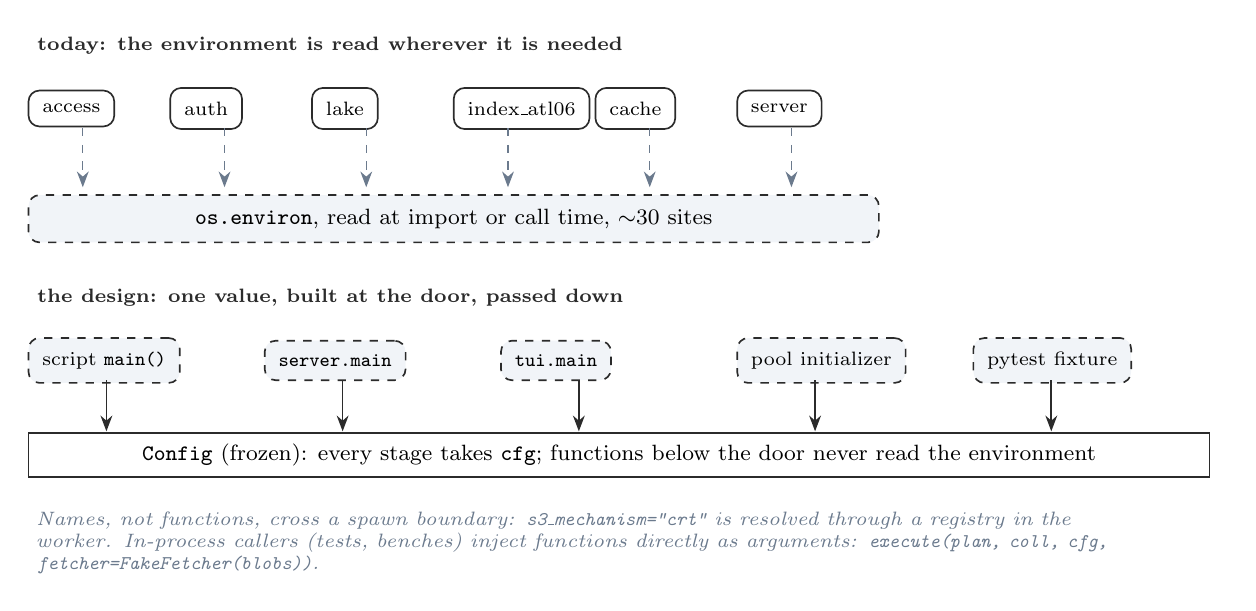
\begin{tikzpicture}[x=1mm,y=1mm]
  \node[hdr] at (0,40) {today: the environment is read wherever it is needed};
  \foreach \x/\t in {0/access, 18/auth, 36/lake, 54/index\_atl06, 72/cache, 90/server} {
    \node[pure, anchor=west, font=\scriptsize] at (\x,32) {\t};
    \draw[flowsoft, dashed] ({\x+7},29.5) -- ({\x+7},22);
  }
  \node[eff, minimum width=108mm, anchor=west] at (0,18) {\code{os.environ}, read at import or call time, $\sim$30 sites};
  \node[hdr] at (0,8) {the design: one value, built at the door, passed down};
  \foreach \x/\t in {0/script \code{main()}, 30/\code{server.main}, 60/\code{tui.main}, 90/pool initializer, 120/pytest fixture} {
    \node[eff, anchor=west, font=\scriptsize] (d\x) at (\x,0) {\t};
    \draw[flow] ({\x+10},-2.5) -- ({\x+10},-9);
  }
  \node[val, minimum width=150mm, anchor=west] at (0,-12) {\code{Config} (frozen): every stage takes \code{cfg}; functions below the door never read the environment};
  \node[note, text width=150mm, anchor=north west] at (0,-18) {Names, not functions, cross a spawn boundary:
    \code{s3\_mechanism="crt"} is resolved through a registry in the worker. In-process callers (tests, benches)
    inject functions directly as arguments: \code{execute(plan, coll, cfg, fetcher=FakeFetcher(blobs))}.};
\end{tikzpicture}}
\caption{Configuration moves from scattered environment reads to one value built at each process door. A
transitional process-wide accessor lets old modules read it until they take \code{cfg} explicitly.}
\label{fig:doors}
\end{figure}

The environment variable names stay as they are, so deployment files are unchanged; what changes is that below
the door nothing reads them. Customisation is by argument, not by subclass or monkeypatch: a different lake layout
is a different \code{Layout} value passed to the lake; a different coalescing policy is a different function passed
to the fetcher; a test's fake archive is a \code{fetcher} argument to the executor. The one transitional concession
is a process-wide accessor returning the config set at the door, which old modules call until they are converted,
and which an AST test forbids in the new packages.

\section{The grid as a parameter}
\label{ch:grid}

Part~\ref{part:dggs} compared four grids and chose H3 on three properties; this chapter says exactly what the design needs from a grid. The
honest list is short, and the performance contract decides what may be abstracted at all.

\begin{lstlisting}
@dataclass(frozen=True, slots=True)
class Grid:                       # one value per implementation
    name: str                     # "h3" | "s2" | "rhealpix"
    resolutions: range
    convex_cells: bool            # may the exact-run shortcut be trusted?
    cell_area_km2: Callable[[int], float]
    cells_vectorized: Callable[[Arr, Arr, int], Arr]       # lat, lon -> ids: THE hot kernel
    cells_for_area: Callable[[Ring, int], Sequence[int]]   # polyfill, overlap semantics
    parent: Callable[[int, int], int]
    children: Callable[[int, int], Sequence[int]]
    compact: Callable[[Sequence[int]], Sequence[int]]      # the claim's representation
    boundary: Callable[[int], Sequence[tuple[float, float]]]
    neighbors: Callable[[int, int], Sequence[int]]
    to_text: Callable[[int], str]; from_text: Callable[[str], int]
\end{lstlisting}

\begin{figure}[tbp]
\centering
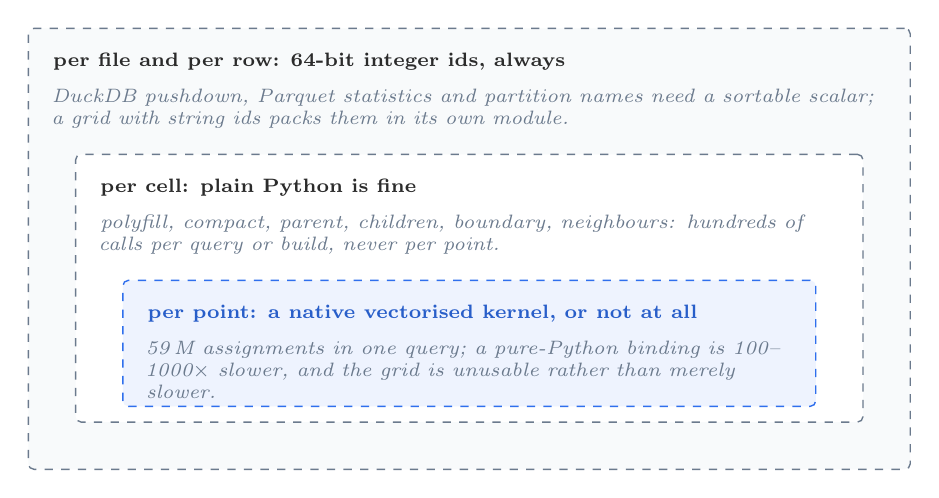
\begin{tikzpicture}[x=1mm,y=1mm]
  \node[proc, minimum width=112mm, minimum height=56mm, anchor=north west, fill=panel!50] (f) at (0,56) {};
  \node[hdr, anchor=north west] at (2,54) {per file and per row: 64-bit integer ids, always};
  \node[note, anchor=north west, text width=104mm] at (2,49.5) {DuckDB pushdown, Parquet statistics and partition
    names need a sortable scalar; a grid with string ids packs them in its own module.};
  \node[proc, minimum width=100mm, minimum height=34mm, anchor=north west, fill=white] (c) at (6,40) {};
  \node[hdr, anchor=north west] at (8,38) {per cell: plain Python is fine};
  \node[note, anchor=north west, text width=92mm] at (8,33.5) {polyfill, compact, parent, children, boundary,
    neighbours: hundreds of calls per query or build, never per point.};
  \node[proc, minimum width=88mm, minimum height=16mm, anchor=north west, fill=idxblue!8, draw=idxblue] (p) at (12,24) {};
  \node[hdr, anchor=north west, text=idxblue!85!black] at (14,22) {per point: a native vectorised kernel, or not at all};
  \node[note, anchor=north west, text width=80mm] at (14,17.5) {59\,M assignments in one query; a pure-Python binding is
    100--1000$\times$ slower, and the grid is unusable rather than merely slower.};
\end{tikzpicture}
\caption{The three cost tiers of grid operations. Only the innermost is performance-critical, and it is the one
operation a grid implementation must provide natively; a descriptor validates it against a time budget on
$10^5$ points at import.}
\label{fig:tiers}
\end{figure}

Three rules follow (Figure~\ref{fig:tiers}). The per-point kernel must be native; a grid without one is rejected,
not tolerated. Per-cell operations run hundreds of times per query and may be plain Python. Storage ids are
64-bit integers whatever the grid's native form, because the index scan, the lake partitions and the manifest all
rely on a sortable scalar; a grid whose ids are strings (rHEALPix's \code{"N2345"}) packs them into 64 bits in its
module and exposes the text form for pages and the API.

The exact-run shortcut of Chapter~\ref{ch:row} rests on one geometric fact, that a straight track meets a cell in
one contiguous stretch, which holds for convex cells. H3 hexagons, S2 cells and rHEALPix cells are convex; a
grid that is not sets \code{convex\_cells} false, which disables the fast path and keeps the per-point fallback.

The grid is part of the store's identity: an index and a lake built under one grid are never read under another,
so the grid's name is recorded beside them and carried in job keys and plans. Column and partition names drop the
grid's name (\code{h3\_cell} becomes \code{cell}), a one-time rename that rides with a schema bump. The addressing
resolution becomes per grid in the descriptor, chosen by the same rule as today, a cell about the footprint of a
chunk: H3 5, S2 9, rHEALPix 4 for ATL06.\side{Adding S2 is a module plus the C++ bindings' vectorised kernel.
rHEALPix has no vectorised kernel in the ecosystem; it is the case that would justify a small Rust extension, which
this structure makes a 200-line package rather than a change to the framework.}

\section{Replay}
\label{ch:replay}

Three values make the system replayable, and each pays for itself in a different place (Figure~\ref{fig:replay}).

\begin{figure}[h]
\wide{%
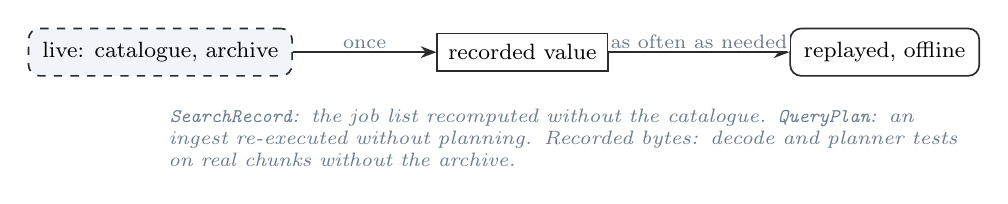
\begin{tikzpicture}[x=1mm,y=1mm]
  \node[eff] (live) at (0,0) {live: catalogue, archive};
  \node[val] (rec) at (46,0) {recorded value};
  \node[pure] (rep) at (92,0) {replayed, offline};
  \draw[flow] (live) -- node[lblw, above] {once} (rec);
  \draw[flow] (rec) -- node[lblw, above] {as often as needed} (rep);
  \node[note, text width=100mm, anchor=north west] at (0,-6) {\code{SearchRecord}: the job list recomputed without
    the catalogue. \code{QueryPlan}: an ingest re-executed without planning. Recorded bytes: decode and planner
    tests on real chunks without the archive.};
\end{tikzpicture}}
\caption{Record once, replay without the effect.}
\label{fig:replay}
\end{figure}

\begin{itemize}
\item \textbf{Build.} A stored \code{SearchRecord} plus the current descriptor and the store's keys recomputes the
  job list exactly. A failed build is re-run from its record; a staleness policy on the record's timestamp decides
  when to search again. The build map that an explainer page reconstructs by hand becomes \code{render(record)}.
\item \textbf{Query.} A \code{QueryPlan} serialises to a directory (the query as JSON, the rows as Arrow) and
  \code{execute(load(plan))} replays it. The ingest benchmark becomes ``record once, execute $N$ times with a
  different writer count'', which is the honest form of the measurement Chapter~\ref{ch:queryruntime} relied on.
\item \textbf{Bytes.} A recording fetcher wraps any fetcher and writes each (url, offset, size) request's bytes to
  a fixture directory. One small granule per collection, recorded once in-region, lets decode and planner tests run
  on real bytes instead of synthetic blobs.
\end{itemize}

\section{Packages and the structural view}
\label{ch:packages}

The code today is one package of 13{,}000 lines whose index, lake, planner, coverage and collection modules form a
single strongly connected import component of thirteen modules. The design splits it along the two seams the
application crosses without the framework (grid geometry and the point cache) and keeps the rest as layers inside
one framework package, separated by import contracts rather than by packaging (Figure~\ref{fig:dag}, Table~\ref{tab:packages}).

\begin{table}[h]
\footnotesize
\wide{\begin{tabular}{@{}llp{52mm}p{40mm}@{}}
\toprule
package & lines & responsibility & who else would use it \\
\midrule
\code{dggs} & $\sim$400 & grid geometry over areas and cell sets; \code{Grid} values for H3 (and later S2) & anyone indexing by a global grid \\
\code{edcloud} & $\sim$900 & Earthdata mechanisms: login, catalogue search to \code{SearchRecord}, range and whole-object GETs, HDF5 chunk maps, decode & any project reading archive granules by byte range \\
\code{pointlake} & $\sim$900 & cell-partitioned Parquet memo, key table, writer, eviction & any cell-keyed point cache \\
\code{cellindex} & $\sim$2\,500 & the framework: descriptor, values, build and query pipelines, store, claim, manifest & another altimetry or lidar project with its own descriptor \\
\code{aicesat} & the rest & scenes, analysis, API, server, TUI, browser, deploy & not reused \\
\bottomrule
\end{tabular}}
\caption{The packages. One repository, one uv workspace; separate repositories only when an external consumer
needs a different release cadence.}
\label{tab:packages}
\end{table}

\begin{figure}[tbp]
\wide{%
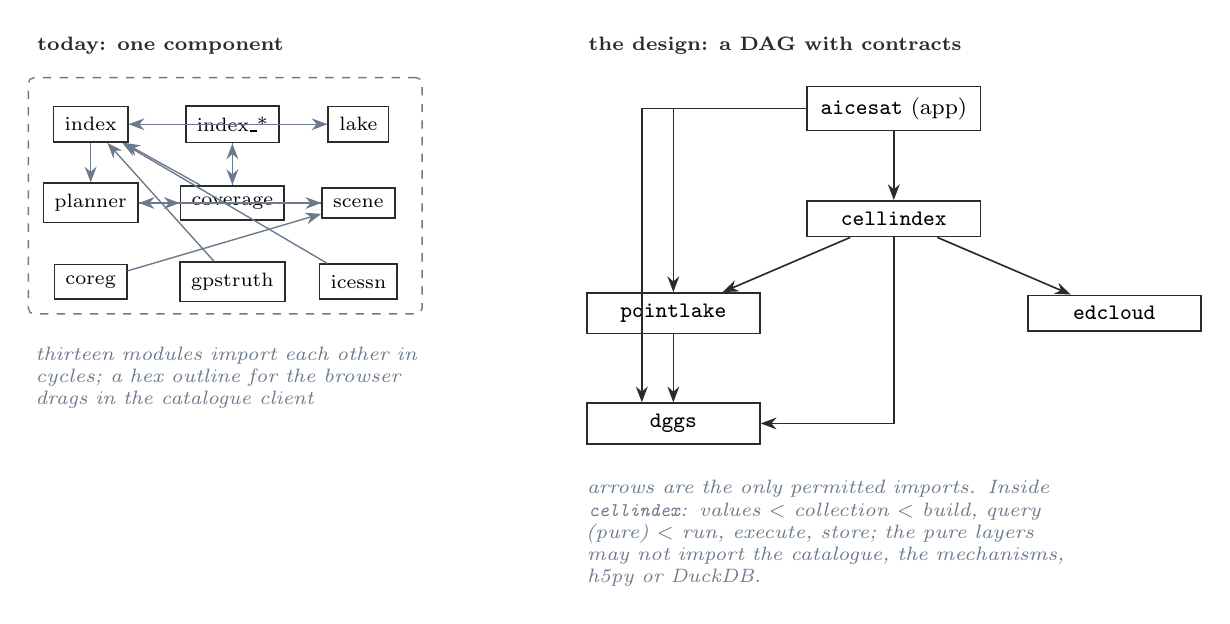
\begin{tikzpicture}[x=1mm,y=1mm]
  \node[hdr] at (0,40) {today: one component};
  \node[proc, minimum width=50mm, minimum height=30mm, anchor=north west] (scc) at (0,36) {};
  \foreach \n/\x/\y/\t in {index/8/30/index, ixs/26/30/index\_*, lake/42/30/lake, planner/8/20/planner, coverage/26/20/coverage, scene/42/20/scene, coreg/8/10/coreg, gpstruth/26/10/gpstruth, icessn/42/10/icessn} {
    \node[val, font=\scriptsize] (\n) at (\x,\y) {\t};
  }
  \foreach \a/\b in {index/lake, lake/index, index/planner, planner/coverage, coverage/index, ixs/coverage, coverage/ixs, scene/planner, planner/scene, coreg/scene, gpstruth/index, icessn/index} {
    \draw[flowsoft] (\a) -- (\b);
  }
  \node[note, text width=50mm, anchor=north west] at (0,3) {thirteen modules import each other in cycles; a hex
    outline for the browser drags in the catalogue client};
  \node[hdr] at (70,40) {the design: a DAG with contracts};
  \node[val, minimum width=22mm] (app) at (110,32) {\code{aicesat} (app)};
  \node[val, minimum width=22mm] (ci) at (110,18) {\code{cellindex}};
  \node[val, minimum width=22mm] (pl) at (82,6) {\code{pointlake}};
  \node[val, minimum width=22mm] (ed) at (138,6) {\code{edcloud}};
  \node[val, minimum width=22mm] (dg) at (82,-8) {\code{dggs}};
  \draw[flow] (app) -- (ci); \draw[flow] (app.west) -| (pl.north); \draw[flow] (app.west) -| ([xshift=-4mm]dg.north);
  \draw[flow] (ci) -- (pl); \draw[flow] (ci) -- (ed); \draw[flow] (pl) -- (dg); \draw[flow] (ci.south) |- (dg.east);
  \node[note, text width=60mm, anchor=north west] at (70,-14) {arrows are the only permitted imports. Inside
    \code{cellindex}: values $<$ collection $<$ build, query (pure) $<$ run, execute, store; the pure layers may not
    import the catalogue, the mechanisms, h5py or DuckDB.};
\end{tikzpicture}}
\caption{Before and after. The cycles of today's single component become a four-package DAG under the
application, with layer contracts inside the framework package.}
\label{fig:dag}
\end{figure}

The mapping from today's modules is direct: \code{access} becomes \code{edcloud} (with the pure parts, coalescing
and decode, separated from the mechanisms); \code{lake} becomes \code{pointlake}; \code{planner}'s geometry
becomes \code{dggs}; \code{index}, \code{index\_*}, \code{build}, \code{pool}, the rest of \code{planner} and the
non-presentation half of \code{coverage} become \code{cellindex}; the analysis modules (co-registration, time
series, lake levels, DEM and imagery readers) stay in the application, already pure at the function level, until a
second consumer appears.

\section{Purity in Python, and what not to do}
\label{ch:discipline}

Python enforces none of the above. The design is kept honest by tools that run in the one check target, since
there is no continuous integration today:

\begin{enumerate}
\item \textbf{Import contracts} (import-linter): the layer order inside \code{cellindex} and the forbidden
  imports listed under Figure~\ref{fig:dag}; the application may not import the build runner from request
  handlers.
\item \textbf{An AST purity test} over the pure module list, failing on environment reads, file opens, clocks,
  randomness, caches, threading and any module-level mutable assignment. The test that today forbids the query
  path from reaching the catalogue is this test's ancestor and is already parsed, not grepped.
\item \textbf{Types}: strict checking on the value modules and the grid package from day one, ratcheted elsewhere.
\item \textbf{Lint rules} that catch the usual leaks: naive clocks, prints in libraries, mutable defaults.
\item \textbf{Frozen, slotted values} with validation in \code{\_\_post\_init\_\_} rather than defensive code
  downstream.
\item \textbf{Coverage floors} per package, and the golden suite (nine numbers against a cloned data directory) as
  the behavioural floor for the application at every migration step.
\end{enumerate}

And the list of things the design deliberately does not do, each of which was considered:

\begin{itemize}
\item No effect system. Values are used in the four places replay or parallelism pays (\code{SearchRecord},
  \code{Job}, \code{QueryPlan}, \code{ChunkWrite}); everywhere else a function that takes \code{cfg} and
  \code{io} arguments is the whole pattern.
\item No class hierarchy and no plugin entry points for collections. A frozen dataclass with function-valued
  fields, one module per collection, pickles across spawn and is all that is needed.
\item No storage interfaces over DuckDB, Parquet or the grid kernel. They \emph{are} the performance; the
  pluggable points are the fetch mechanism, the layout value, the cell kernel and the coalescing policy, each a
  plain argument.
\item No repository split, package index or independent versioning before a second consumer exists.
\item No ``pure'' writer. The queue's backpressure is what bounds memory.
\item No refactoring of the leaf kernels (decode, coalesce, span cutting, the parsers). They are the parts that
  are already right.
\item No trust in purity by convention. Hence the list above.
\end{itemize}

\appendix
\clearpage

\part*{Appendices}
\addcontentsline{toc}{part}{Appendices}

\section{Migration path}
\label{app:migration}

Each step lands on the main branch, passes the full suite and the golden suite, and deploys. Steps are ordered so
that each removes a hazard on its own (Table~\ref{tab:migration}).

\begin{center}
\footnotesize
\wide{\begin{tabular}{@{}lp{52mm}p{38mm}cp{34mm}@{}}
\toprule
step & what & retires & effort & status \\
\midrule
A & \code{Config} at the doors; \code{from\_sources}; \code{cfg} threaded through the fetcher, lake and planner; transitional accessor & environment reads below the doors & 2\,d & \\
B & \code{GranuleRef} and \code{Job}; one \code{run\_build}; spawn pool with deadline and retry; resolution guard in every builder & five drivers, five fork pools, per-task pickling of the cell set & 3\,d & partly landed 2026-10-17; \code{SearchRecord} and the pool initializer remain \\
C & \code{SearchRecord} stored; the claim as a fold writing today's file shape & claim mutation, claim invalidation, the catalogue pickle & 2\,d & \\
D & content-addressed index store; manifest rows carry keys; glob fallbacks deleted; explicit conservative GC; one-shot rename on the box & six resume sets, footer provenance reads, the sidecars (the sha is in the key) & 4\,d & highest risk: 120k files renamed; rehearse on the clone \\
E & \code{Collection} descriptor and one \code{build\_job} with three layouts; \code{Grid} enters here & six builder bodies, per-collection version constants & 3\,d & \\
F & \code{QueryPlan}, one \code{execute}, one \code{keep}; the lake takes a cell column & five fetch loops, five keep predicates, the ATL03 variant & 5\,d & seeds landed: one cell pass, group files, runs \\
G & extract packages; uv workspace; import contracts; delete the accessor & module singletons as cross-package state & 3\,d & \\
H & application split: scenes, analysis, admin; presentation registry; TUI over the public API & duplicated mission tables & 4\,d & \\
\bottomrule
\end{tabular}}
\captionof{table}{About 26 days of focused work; D and F carry the least trustworthy estimates.}
\label{tab:migration}
\end{center}

\section{Test strategy}
\label{app:tests}

Table~\ref{tab:tests} gives the shape of the tests per package and the coverage floor each must hold.

\begin{center}
\footnotesize
\wide{\begin{tabular}{@{}lp{44mm}p{44mm}p{36mm}c@{}}
\toprule
package & pure-core tests & interpreter tests & property tests & floor \\
\midrule
\code{dggs} & literal geometry; claim compaction & none & compact and membership preserve every cell; polyfill covers centre-contained cells; the kernel agrees with the scalar API and meets the time budget & 100\,\% \\
\code{edcloud} & coalesce, decode, span cutting on literals and recorded blobs & mechanisms behind a fake archive; catalogue with fixtures; token parsing & coalesce covers every input and respects the gap; decode$\circ$encode identity with shuffle and gzip & 95 / 80\,\% \\
\code{pointlake} & cell tables with a cell column; dtype preservation & writer ordering, eviction, stats, query scoping under a temporary config & write then query returns the same multiset & 90\,\% \\
\code{cellindex} & jobs from literal records; rows from positions; plan on Arrow literals (todo$\,\cap\,$have $= \emptyset$, every wanted cell is in lake or todo); keep; claim fold & \code{build\_job} with a fake io (in-memory HDF5 plus recorded blobs); \code{run\_build} with an inline pool; \code{execute} with a fake fetcher, byte-identical to the direct fetch for all six collections & job key stable under field order; plan idempotent & 95 / 85\,\% \\
\code{aicesat} & science modules as they are & API, server, stream, TUI as they are; golden suite unchanged at every step & & 85\,\% \\
\bottomrule
\end{tabular}}
\captionof{table}{Per-package test shape and coverage floors. Of today's $\sim$10\,500 test lines, about 1\,900 move with
their modules, about 1\,200 retire with what they tested, and the rest stay in the application.}
\label{tab:tests}
\end{center}

\section{Measurements the design leans on}
\label{app:numbers}

Table~\ref{tab:numbers} collects every number the text relies on, with the instrument that produced it.

\begin{center}
\footnotesize
\wide{\begin{tabular}{@{}p{66mm}rrp{44mm}@{}}
\toprule
measurement & before & after & instrument \\
\midrule
ATL06 build, 100 granules, 8 workers & 44.7\,s & 21.3\,s & \code{bench\_build\_io.py} \\
ATL06 build, workers 4 / 8 / 16 / 32 (before whole object) & \multicolumn{2}{c}{81 / 42 / 26 / 26\,s} & \code{bench\_build\_io.py} \\
ATL06 per granule, serial reads through the block cache & \multicolumn{2}{c}{66 reads, 2.0\,s} & profile \\
ATL06 full regional rebuild, 33\,484 granules & 3.9\,h & 62\,min & staging rebuild \\
GLAS full rebuild, 4\,799 granules & 10\,min & 3.5\,min & staging rebuild \\
ATL03 structure reads per granule at 1 / 4 / 16\,MiB blocks & \multicolumn{2}{c}{114 / 7 / 4} & \code{bench\_build\_io.py} \\
16 spawned workers, peak memory & & 3.4\,GB & \code{free -m} \\
8-cell ATL06 ingest, wall & 25.4\,s & 16.6\,s & \code{bench\_ingest\_fresh.py} \\
same, CPU-seconds & 40.7 & 32.4 & idem \\
same, CPU-s / wall-s (2 physical cores) & & 2.45 & idem \\
same, lake files written & 6\,897 & 3\,225 & idem \\
same, cell assignment thread-seconds & 24--31 & 0 & idem; 2\,948 of 2\,948 chunks from runs \\
exact runs on real ATL06 rows (12 granules) & & 99.3\,\% & \code{tests/test\_index\_cell\_runs.py} \\
ATL03 plan for a 0.3$^\circ$ box & 36\,s & 0.66\,s & query trace \\
index store with sidecar provenance & 7.5\,GB & 4.7\,GB & \code{migrate\_index\_footers.py} \\
in-region fetch throughput, CRT client & 300--400 & 670--840\,MB/s & \code{bench\_coalesce.py} \\
precache-adjacent, first box / neighbour (on vs off) & 16.8 / 13.9\,s & 31.9 / 21.7\,s & \code{bench\_ingest\_fresh.py} \\
\midrule
catalogue hits for a 2$^\circ$ box, ATL06 / ATL03 / GLAS & \multicolumn{2}{c}{549--571 / 560--602 / 93--139} & \code{measure\_search\_modes.py} \\
bytes moved by whole-granule retrieval vs needed, ATL06 / ATL03 & \multicolumn{2}{c}{63--80$\times$ / 70--94$\times$} & idem \\
same, the 15\,km transect box, ATL06 / ATL03 & \multicolumn{2}{c}{86$\times$ / 475$\times$} & idem \\
catalogue hits with no point in the box's cells, ATL06 / GLAS & \multicolumn{2}{c}{9.6--31.8\,\% / 8.6--32.3\,\%} & idem \\
granule footprint area over box area, ICESat-2, 2$^\circ$ box / transect & \multicolumn{2}{c}{7.2--9.8$\times$ / 852--1\,009$\times$} & idem \\
ATL06 granule size over Greenland, quartiles & \multicolumn{2}{c}{72 / 88 / 96\,MB} & idem \\
ATL03 granule size over Summit, quartiles & \multicolumn{2}{c}{0.95 / 1.4 / 2.7\,GB} & idem \\
ATL03 staging rebuild, 48\,838 granules, 16 workers, 4\,MiB blocks & 12\,h & 7.4\,h & staging rebuild, 2026-10-18 \\
\bottomrule
\end{tabular}}
\captionof{table}{Measurements on the deployed instance (m6i.xlarge, 4 vCPU, 15\,GB, us-west-2), 2026-10-16 to 19. The search-mode rows are the full table of \code{docs/notes/search-modes-2026-10.md}.}
\label{tab:numbers}
\end{center}

\section{Glossary}
\label{app:glossary}

\begin{description}\setlength{\itemsep}{1pt}
\item[along-track] data ordered by time along a ground track, with position stored per measurement.
\item[footprint] (of a measurement) the ground patch one laser pulse illuminates; (of a granule) the catalogued extent.
\item[granule] one archive file: an orbit region, an orbit arc, minutes of a flight, a survey.
\item[RGT, cycle, region] ICESat-2's reference ground track (1 of 1\,387), its 91-day repeat count, and one of the 14 latitude cuts of an orbit.
\item[campaign] a GLAS laser operating period (19, L1A--L2F) or an IceBridge season.
\item[platelet] one ILATM2 record: a plane fitted to a block of ATM points, 80\,m across at nadir.
\item[DGGS] discrete global grid system: nested partitions of the Earth with an identifier scheme.
\item[aperture] the number of children a grid cell has at the next resolution (H3: 7).
\item[polyfill] the set of cells an area overlaps.
\item[compaction] replacing every complete set of children in a cell set by their parent, recursively.
\item[over-claim] a catalogued footprint larger than the ground the granule measured; a false positive is a search hit with no point in the area.
\item[chunk] a fixed-size, separately compressed piece of an HDF5 dataset; the unit of a byte range.
\item[chunk map] (offset, size, filters) for every chunk of a dataset, read from the file's B-tree once at build.
\item[span] GEDI's row unit: an element interval inside one chunk of every dataset.
\item[cell] a grid cell at some resolution; addressing cells key rows and lake files, claim cells record coverage.
\item[run] the element interval of one cell inside one chunk, and whether it is pure.
\item[index] one Parquet file per granule of (chunk, cell) rows carrying byte ranges and runs.
\item[claim] the compacted cell set a collection's index is known to cover; consulted before every query.
\item[manifest] the fold of an index into distinct (cell, granule, month) rows; names the files a query opens.
\item[provenance] the filter set a granule's file was built against, recorded in its footer by hash.
\item[lake] the cell-partitioned Parquet memo of decoded points, read before and written after a fetch.
\item[beam group] the set of beams the planner requests together and the lake files together.
\item[have, todo] the chunks a plan serves from the lake, and those it fetches.
\item[door] a process entry point where configuration is built once: a script's main, the server, the TUI, a
  pool initializer, a test fixture.
\item[slot] a function-valued field of a collection descriptor that a pipeline stage calls.
\item[value] immutable data; a frozen dataclass here.
\item[effect] a function that touches the network, the disk, a clock or a pool.
\end{description}

\clearpage
\bibliographystyle{unsrt}
\bibliography{functional-design}
\addcontentsline{toc}{section}{References}

\end{document}
